\documentclass[twocolumn]{aastex701}
%\usepackage{apjfonts}
\usepackage{graphicx}
\usepackage{color}
\usepackage{amsmath}
\usepackage{mathtools}
\usepackage{tcolorbox}
\usepackage{gensymb}

\usepackage{listings}

\shorttitle{Binary Orbits}
\shortauthors{Bhadra et al.}

\definecolor{codegreen}{rgb}{0,0.6,0}
\definecolor{codegray}{rgb}{0.3,0.3,0.3}
\definecolor{codepurple}{rgb}{0.58,0,0.82}
\definecolor{backcolour}{rgb}{0.9,0.9,0.9}

\lstdefinestyle{mystyle}{
    backgroundcolor=\color{backcolour},   
    commentstyle=\color{codegreen},
    keywordstyle=\color{magenta},
    numberstyle=\tiny\color{codegray},
    stringstyle=\color{codepurple},
    basicstyle=\ttfamily\footnotesize,
    breakatwhitespace=false,         
    breaklines=true,                 
    captionpos=b,                    
    keepspaces=true,                 
    numbers=left,                    
    numbersep=5pt,                  
    showspaces=false,                
    showstringspaces=false,
    showtabs=false,                  
    tabsize=2
}

\lstset{style=mystyle}

\newcommand{\geotr}{\earth_r}
\newcommand{\norm}[1]{\lVert#1\rVert}
\newcommand{\vect}[1]{\boldsymbol{#1}}
\newcommand{\murel}{\mu_{\mathrm{rel},\sun}}
\newcommand{\acc}{a_{s,\sun}}
\newcommand{\murelsec}{\mu_{\mathrm{rel},s,\sun}}

\newcommand{\murelE}{\mu_{\mathrm{rel},\sun,E}}
\newcommand{\murelN}{\mu_{\mathrm{rel},\sun,N}}
\newcommand{\murelgeo}{\mu_{\mathrm{rel},\earth}}
\newcommand{\murelgeotr}{\mu_{\mathrm{rel},\geotr}}
\newcommand{\murelgeotrE}{\mu_{\mathrm{rel},\geotr,E}}
\newcommand{\murelgeotrN}{\mu_{\mathrm{rel},\geotr,N}}
\newcommand{\murelvec}{\vect{\mu}_{\boldsymbol{\mathrm{rel}},\sun}}
\newcommand{\murelsecvec}{\vect{\mu}_{\boldsymbol{\mathrm{rel}},s,\sun}}
\newcommand{\accSsec}{\bold{a}_{\boldsymbol{S\mathrm{rel}},\sun}}
\newcommand{\accLsec}{\bold{a}_{\boldsymbol{L\mathrm{rel}},\sun}}
\newcommand{\murelvecgeo}{\vect{\mu}_{\boldsymbol{\mathrm{rel}},\earth}}
\newcommand{\murelvecgeotr}{\vect{\mu}_{\boldsymbol{\mathrm{rel}},\geotr}}
\newcommand{\thetaEhat}{\boldsymbol{\hat{\theta}}_{\boldsymbol{E}}}
\newcommand{\murelhat}{\boldsymbol{\hat{\mu}}_{\boldsymbol{\mathrm{rel}},\sun}}
\newcommand{\murelsechat}{\boldsymbol{\hat{\mu}}_{\boldsymbol{\mathrm{rel}},s,\sun}}
\newcommand{\accrelhat}{\boldsymbol{\hat{a}}_{s,\sun}}
\newcommand{\murelhatE}{\hat{\mu}_{\mathrm{rel},\sun,E}}
\newcommand{\murelhatN}{\hat{\mu}_{\mathrm{rel},\sun,N}}
\newcommand{\murelhatgeotr}{\boldsymbol{\hat{\mu}}_{\boldsymbol{\mathrm{rel}},\geotr}}
\newcommand{\murelhatgeotrE}{\hat{\mu}_{\mathrm{rel},\geotr,E}}
\newcommand{\murelhatgeotrN}{\hat{\mu}_{\mathrm{rel},\geotr,N}}
\newcommand{\tnot}{t_{0,\sun}}
\newcommand{\uvecohat}{\boldsymbol{\hat{u}}_{\boldsymbol{0},\sun}}
\newcommand{\uvecohatcom}{\boldsymbol{\hat{u}}_{\boldsymbol{0, com},\sun}}

\newcommand{\uvecohatgeotr}{\vect{\hat{u}}_{\boldsymbol{0},\geotr}}
\newcommand{\thetaevec}{\vect{\theta}_{\boldsymbol{E}}}
\newcommand{\uvec}{\vect{u}_{\sun}}
\newcommand{\uvecgeo}{\vect{u}_{\earth}}
\newcommand{\uvecgeotr}{\vect{u}_{\geotr}}
\newcommand{\uveco}{\vect{u}_{\boldsymbol{0},\sun}}
\newcommand{\uvecogeo}{\vect{u}_{\boldsymbol{0},\earth}}
\newcommand{\uvecogeotr}{\vect{u}_{\boldsymbol{0},\geotr}}
\newcommand{\uE}{u_{\sun,E}}
\newcommand{\uN}{u_{\sun,N}}
\newcommand{\ugeotrE}{u_{\geotr,E}}
\newcommand{\ugeotrN}{u_{\geotr,N}}
\newcommand{\uoE}{u_{0,\sun,E}}
\newcommand{\uoN}{u_{0,\sun,N}}
\newcommand{\uogeotrE}{u_{0,\geotr,E}}
\newcommand{\uogeotrN}{u_{0,\geotr,N}}
\newcommand{\deltavec}{\vect{\delta}_{\boldsymbol{c}}}
\newcommand{\OBtwotwo}{OGLE-2011-BLG-0022}
\newcommand{\OBtwofive}{OGLE-2011-BLG-0125}
\newcommand{\OBsixnine}{OGLE-2012-BLG-0169}
\newcommand{\tE}{t_{E,\sun}}
\newcommand{\tEsec}{t_{E,sec,\sun}}
\newcommand{\tEgeotr}{t_{E,\geotr}}
\newcommand{\thetaE}{\theta_E}
\newcommand{\uo}{u_{0,\sun}}
\newcommand{\uocom}{u_{com, 0,\sun}}

\newcommand{\uogeotr}{u_{0,\geotr}}
\newcommand{\uoplus}{u_0^+}
\newcommand{\uominus}{u_0^-}
\newcommand{\rhostar}{\rho_{\star}}
\newcommand{\thetastar}{\theta_{\star}}
\newcommand{\vtildevec}{\vect{\tilde{v}}}
\newcommand{\vtilde}{\tilde{v}}
\newcommand{\piEvec}{\vect{\pi}_{E,\sun}}
\newcommand{\piEvecgeotr}{\vect{\pi}_{E,\geotr}}
\newcommand{\piE}{\pi_E}
\newcommand{\piEhat}{\hat{\boldsymbol{\pi}}_{E,\sun}}
\newcommand{\pirel}{\pi_{\mathrm{rel}}}
\newcommand{\tnaught}{t_{0,\sun}}
\newcommand{\tnotgeotr}{t_{0,\geotr}}
\newcommand{\fsrc}{f_{S}}
\newcommand{\fb}{f_{b}}
\newcommand{\piEN}{\pi_{E, N}}
\newcommand{\piEE}{\pi_{E, E}}
\newcommand{\deltachisq}{\Delta\chi^2}
\newcommand{\chisquare}{\chi^2}
\newcommand{\subsun}{_{\odot}}
\newcommand{\x}{E}
\newcommand{\y}{N}
\newcommand{\sigmaX}{\sigma_{\x, i}}
\newcommand{\sigmaY}{\sigma_{\y, i}}
\newcommand{\xpos}{x_{\x}}
\newcommand{\ypos}{x_{\y}}
\newcommand{\xobs}{x_\x^\mathrm{obs}}
\newcommand{\yobs}{x_\y^\mathrm{obs}}
\newcommand{\tobs}{t^\mathrm{obs}}
\newcommand{\xobsi}{x_{\x, i}^{\mathrm{obs}}}
\newcommand{\yobsi}{x_{\y, i}^{\mathrm{obs}}}
\newcommand{\tobsi}{t_{i}^{\mathrm{obs}}}
\newcommand{\xmodi}{x_{\x, i}^{\mathrm{mod}}}
\newcommand{\ymodi}{x_{\y, i}^{\mathrm{mod}}}
\newcommand{\tmodi}{t_{i}^{\mathrm{mod}}}
\newcommand{\musvec}{\vect{\mu}_{\boldsymbol{S},\sun}}
\newcommand{\mussysvec}{\vect{\mu}_{\boldsymbol{S, com},\sun}}
\newcommand{\mulsysvec}{\vect{\mu}_{\boldsymbol{L, com},\sun}}


\newcommand{\mulsysvece}{{\mu}_{{L, com, e},\sun}}


\newcommand{\mulsysvecn}{{\mu}_{{L, com, n},\sun}}


\newcommand{\mussysvece}{\mu_{{S, E, com},\sun}}

\newcommand{\mussysvecn}{\mu_{{S, n, com},\sun}}

\newcommand{\mussvec}{\vect{\mu}_{\boldsymbol{S_s},\sun}}
\newcommand{\deltamussvec}{\vect{\Delta\mu}_{\boldsymbol{S_s},\sun}}

\newcommand{\deltamulsvec}{\vect{\Delta\mu}_{\boldsymbol{L_s},\sun}}


\newcommand{\mulvec}{\vect{\mu}_{\boldsymbol{L},\sun}}

\newcommand{\mulsvec}{\vect{\mu}_{\boldsymbol{L_s} ,\sun}}

\newcommand{\Xsovec}{\vect{X}_{\boldsymbol{S,0},\sun}}
\newcommand{\Xlovec}{\vect{X}_{\boldsymbol{L,0},\sun}}
\newcommand{\Xsvec}{\vect{X}_{\boldsymbol{S},\sun}}
\newcommand{\Xlvec}{\vect{X}_{\boldsymbol{L},\sun}}
\newcommand{\Xsvecgeo}{\vect{X}_{\boldsymbol{S},\earth}}
\newcommand{\Xlvecgeo}{\vect{X}_{\boldsymbol{L},\earth}}
\newcommand{\Pvec}{\vect{P}}
\newcommand{\Pdotvec}{\vect{\dot{P}}}
\newcommand{\PE}{P_E}
\newcommand{\PN}{P_N}
\newcommand{\PdotE}{\dot{P}_E}
\newcommand{\PdotN}{\dot{P}_N}
\newcommand{\bsff}{b_{sff}}



\newcommand{\Xspovec}{\vect{X}_{\boldsymbol{S_p,0},\sun}}

\newcommand{\Xlpovec}{\vect{X}_{\boldsymbol{L_p,0},\sun}}


\newcommand{\Xscomvec}{\vect{X}_{\boldsymbol{S_{com},0},\sun}}
\newcommand{\Xlcomvec}{\vect{X}_{\boldsymbol{L_{com},0},\sun}}
\newcommand{\Xlcomvece}{\vect{X}_{\boldsymbol{L_{com},e,0},\sun}}
\newcommand{\Xlcomvecn}{\vect{X}_{\boldsymbol{L_{com},n,0},\sun}}

\newcommand{\Xscomvece}{\vect{X}_{\boldsymbol{S_{com}, e, 0},\sun}}
\newcommand{\Xscomvecn}{\vect{X}_{\boldsymbol{S_{com}, n, 0},\sun}}
\newcommand{\Xssovec}{\vect{X}_{\boldsymbol{S_s,0},\sun}}
\newcommand{\Xlsovec}{\vect{X}_{\boldsymbol{L_s,0},\sun}}

\newcommand{\Xspvec}{\vect{X}_{\boldsymbol{S_p},\sun}}

\newcommand{\XIvec}{\vect{X}_{\boldsymbol{S, I},\sun}}

\newcommand{\Xlpvec}{\vect{X}_{\boldsymbol{L_p},\sun}}
\newcommand{\Xlsvec}{\vect{X}_{\boldsymbol{L_s},\sun}}


\newcommand{\Xspveccom}{\vect{X(t)}_{\boldsymbol{S_p, com},\sun}}
\newcommand{\Xssveccom}{\vect{X(t)}_{\boldsymbol{S_s, com},\sun}}
\newcommand{\Xspveccome}{\vect{X(t)}_{\boldsymbol{S_p, E, com},\sun}}
\newcommand{\Xspveccomn}{\vect{X(t)}_{\boldsymbol{S_p, N, com},\sun}}
\newcommand{\Xssveccome}{\vect{X(t)}_{\boldsymbol{S_s, E, com},\sun}}
\newcommand{\Xssveccomn}{\vect{X(t)}_{\boldsymbol{S_s, N, com},\sun}}
\newcommand{\Xspvece}{\vect{X(t)}_{\boldsymbol{S_p, E},\sun}}
\newcommand{\Xspvecn}{\vect{X(t)}_{\boldsymbol{S_p, N},\sun}}
\newcommand{\Xssvece}{\vect{X(t)}_{\boldsymbol{S_s, E},\sun}}
\newcommand{\Xssvecn}{\vect{X(t)}_{\boldsymbol{S_s, N},\sun}}


\newcommand{\Xcomp}{\vect{X(t)}_{\boldsymbol{p},\boldsymbol{com},\sun}}
\newcommand{\Xcoms}{\vect{X(t)}_{\boldsymbol{s},\boldsymbol{com},\sun}}


\newcommand{\Xcomep}{{X(t)}_{{p, {com}, E},\sun}}
\newcommand{\Xcomnp}{{X(t)}_{{p, {com}, N},\sun}}

\newcommand{\Xcomes}{{X(t)}_{{s, {com}, E},\sun}}
\newcommand{\Xcomns}{{X(t)}_{{s, {com}, N},\sun}}



\newcommand{\Xlpvece}{\vect{X(t)}_{\boldsymbol{L_p, E},\sun}}
\newcommand{\Xlpvecn}{\vect{X(t)}_{\boldsymbol{L_p, N},\sun}}
\newcommand{\Xlsvece}{\vect{X(t)}_{\boldsymbol{L_s, E},\sun}}
\newcommand{\Xlsvecn}{\vect{X(t)}_{\boldsymbol{L_s, N},\sun}}



\newcommand{\Xssvec}{\vect{X}_{\boldsymbol{S_s},\sun}}
\newcommand{\Xspvecgeo}{\vect{X}_{\boldsymbol{S_p},\earth}}
\newcommand{\Xssvecgeo}{\vect{X}_{\boldsymbol{S_s},\earth}}
\newcommand{\upvec}{\vect{u}_{p,\sun}}
\newcommand{\usvec}{\vect{u}_{s,\sun}}
\newcommand{\upvecgeo}{\vect{u}_{p,\earth}}
\newcommand{\usvecgeo}{\vect{u}_{s,\earth}}
\newcommand{\upvecgeotr}{\vect{u}_{p,\geotr}}
\newcommand{\usvecgeotr}{\vect{u}_{s,\geotr}}
\newcommand{\upveco}{\vect{u}_{p,\boldsymbol{0},\sun}}
\newcommand{\usveco}{\vect{u}_{s,\boldsymbol{0},\sun}}
\newcommand{\upvecogeo}{\vect{u}_{p,\boldsymbol{0},\earth}}
\newcommand{\usvecogeo}{\vect{u}_{s,\boldsymbol{0},\earth}}
\newcommand{\upvecogeotr}{\vect{u}_{p,\boldsymbol{0},\geotr}}
\newcommand{\usvecogeotr}{\vect{u}_{s,\boldsymbol{0},\geotr}}
\newcommand{\up}{u_{p,\sun}}
\newcommand{\us}{u_{s,\sun}}
\newcommand{\upE}{u_{p,\sun,E}}
\newcommand{\usE}{u_{s,\sun,E}}
\newcommand{\upN}{u_{p,\sun,N}}
\newcommand{\usN}{u_{s,\sun,N}}
\newcommand{\upgeo}{u_{p,\earth}}
\newcommand{\usgeo}{u_{s,\earth}}
\newcommand{\upgeotrE}{u_{p,\geotr,E}}
\newcommand{\usgeotrE}{u_{s,\geotr,E}}
\newcommand{\upgeotrN}{u_{p,\geotr,N}}
\newcommand{\usgeotrN}{u_{s,\geotr,N}}
\newcommand{\upoE}{u_{p,0,\sun,E}}
\newcommand{\usoE}{u_{s,0,\sun,E}}
\newcommand{\upoN}{u_{p,0,\sun,N}}
\newcommand{\usoN}{u_{s,0,\sun,N}}
\newcommand{\upogeotrE}{u_{p,0,\geotr,E}}
\newcommand{\usogeotrE}{u_{s,0,\geotr,E}}
\newcommand{\upogeotrN}{u_{p,0,\geotr,N}}
\newcommand{\usogeotrN}{u_{s,0,\geotr,N}}
\newcommand{\deltavecp}{\vect{\delta}_{p,\boldsymbol{c}}}
\newcommand{\deltavecs}{\vect{\delta}_{s,\boldsymbol{c}}}
\newcommand{\upo}{u_{p,0,\sun}}
\newcommand{\uso}{u_{s,0,\sun}}
\newcommand{\upogeotr}{u_{p,0,\geotr}}
\newcommand{\usogeotr}{u_{s,0,\geotr}}
\newcommand{\upoplus}{u_{p,0}^+}
\newcommand{\usoplus}{u_{s,0}^+}
\newcommand{\upominus}{u_{p,0}^-}
\newcommand{\usominus}{u_{s,0}^-}
\newcommand{\upplus}{\boldsymbol{u_{p}^+}}
\newcommand{\usplus}{\boldsymbol{u_{s}^+}}
\newcommand{\upminus}{\boldsymbol{u_{p}^-}}
\newcommand{\usminus}{\boldsymbol{u_{s}^-}}

\newcommand{\tpnot}{t_{prim,0,\sun}}
\newcommand{\tcomnot}{t_{com,0,\sun}}
\newcommand{\tsnot}{t_{s,0,\sun}}


\newcommand{\w}{\omega_{pri}}
\newcommand{\wsec}{\omega_{sec}}
\newcommand{\bigomega}{\Omega_{sec}}
\newcommand{\bigomegapri}{\Omega_{pri}}
\newcommand{\inclination}{\textit{i}}
\newcommand{\eccentricity}{\textit{e}}
\newcommand{\period}{\textit{P}}
\newcommand{\tp}{\textit{tp}}

\newcommand{\al}{\aleph_{pri}}
\newcommand{\ala}{\aleph_{sec}}
\newcommand{\E}{\textit{E(t)}}
\newcommand{\M}{\textit{M(t)}}

\newcommand{\etanom}{\eta}

\newcommand{\Apri}{A_{pri}}
\newcommand{\Asec}{A_{sec}}
\newcommand{\Bpri}{B_{pri}}
\newcommand{\Bsec}{B_{sec}}

\newcommand{\Cpri}{C_{pri}}
\newcommand{\Csec}{C_{sec}}
\newcommand{\Fpri}{F_{pri}}
\newcommand{\Fsec}{F_{sec}}
\newcommand{\Gpri}{G_{pri}}
\newcommand{\Gsec}{G_{sec}}
\newcommand{\Hpri}{H_{pri}}
\newcommand{\Hsec}{H_{sec}}

\newcommand{\baglett}{{\tt bagle}}
\newcommand{\bagle}{BAGLE}

\newcommand{\berkeley}{\affiliation{Department of Astronomy, University of California, Berkeley, CA 94720, USA}}

\begin{document}

\title{Modeling Binary Lenses and Sources with the BAGLE Python Package}
%\shortitle{Binary Systems}
\author[0009-0002-6097-9030]{T. Dex Bhadra}
\affiliation{Department of Astronomy, University of Maryland, College Park, MD 20742, USA}
\affiliation{Code 667, NASA Goddard Space Flight Center, Greenbelt, MD 20771, USA}
\email{tmbhadra@umd.edu}

\author[0000-0001-9611-0009]{J. R. Lu}
\berkeley
\email{}

\author[0000-0002-0287-3783]{Natasha S. Abrams}
\berkeley
\email{}


\author[0000-0002-1395-5426]{Andrew Scharf}
\affiliation{Department of Mathematics, University of California, Berkeley, CA 94720, USA}
\email{scharfa@berkeley.edu}


\author[0000-0003-0652-1862]{Edward Broadberry} % finite source
\affiliation{Department of Astronomy, University of Maryland, College Park, MD 20742, USA}
\email{edbroad@umd.edu}

\author[0000-0002-6406-1924]{Casey Lam}
\affiliation{Observatories of the Carnegie Institution for Science, Pasadena, CA 91101, USA}
\email{}

\author[0000-0003-4591-3201]{Macy J. Huston}
\berkeley
\email{mhuston@berkeley.edu}

\date{\today}

\begin{abstract}

%In this paper, we describe model parameterizations and lensing equations for binary source and lens models in the Bayesian Analysis of Gravitational Lensing Events (BAGLE) Python microlensing package. At long-duration microlensing events, when the orbital period approaches the duration of the microlensing event, it is important to consider the orbital dynamics of the involved binary system. Therefore, the new binary source and lens models in BAGLE  account for the complete Keplerian orbit, and its derivative linear, accelerated, and circular approximations. Using these additions to \bagle, we explore the impact of binary orbits on photometric and astrometric microlensing signals. 


Gravitational microlensing is a powerful tool that can be used to find and measure the mass of isolated and dark compact objects, including black holes. In many microlensing events, the lens, the source, or both may be a binary system. Therefore, in this study we present lensing equations for binary source and lens models in the Bayesian Analysis of Gravitational Lensing Events (BAGLE) Python microlensing package. These include the binary orbital motion required to measure many long duration, black hole microlensing events. The new binary source and lens models in BAGLE account for the complete Keplerian orbit. BAGLE also includes binary models that approximate the orbital motion as linear or accelerating motion of the secondary companion; these are useful when the orbit has a very low eccentricity or the orbital period is much longer than the microlensing timescale. The model parameterizations based on these binary lensing equations will enable joint fitting of photometric and astrometric data sets. These binary models will be used to fit microlensing event data from the Vera C. Rubin Observatory, the Nancy Grace Roman Telescope, and other surveys. 

%and its derivative linear, accelerated, and circular approximations. These approximations are simplified models that treat the orbital trajectories of the binary system as linear, accelerated or circular; 
\end{abstract}


\section{Introduction
\label{sec:introduction}}

Gravitational microlensing occurs in the Milky Way when a foreground object with mass (e.g., a star, black hole, or planet) passes in front of a background source star and the mass of the foreground lens temporarily magnifies and perturbs the observed position of the background source. 
Microlensing is detectable even when the foreground lens is dark or too faint to observe, making it a powerful tool for probing cool, distant, and/or compact objects. It is one of the only methods for measuring the mass of isolated and dark black holes \citep{Lam:2022, Sahu:2022, Mroz:2022, Lam:2023-OB110462, Sahu2025}, free-floating or widely separated low-mass exoplanets \citep{Gaudi2012}, and white dwarfs \citep{Sahu2017, McGill2023}. Additionally, over 200 exoplanets orbiting their host stars have been detected with microlensing \citep{Mroz_2024}.

Microlensing is sensitive to both close and wide separation binaries, unlike radial velocity and transit probes, which are more sensitive to closely separated binaries or planet+star systems.
Recent simulations of Milky Way microlensing surveys show that 55 \% of observed microlensing events involve a binary star system \citep{Natasha_2025}, so robust binary microlensing models are even more important than previously thought. 
Some microlensing events have timescales greater than the orbital period of the involved binary system. In these cases, photometric lightcurves and astrometric trajectories can only be properly modeled by accounting for the system's orbital dynamics.

There are numerous software packages that encode the math necessary to model and fit a microlensing event such as 
BAGLE \citep{Lu:2025},
pyLIMA \citep{Bachelet2017}, VBMicrolensing \citep{Bozza2010,Bozza2018,Bozza2021,Bozza2024}, and MulensModel \citep{Poleski2019}.
These packages are all publicly available and have their own strengths and weaknesses in terms of the types of event geometries they support, whether they include both photometry and astrometry in their models, and how accurate and efficient their model-fitting capabilities are. A detailed comparison of these packages for point-source, point-lens models is presented in \citep{Lu:2025}. PyLIMA, VBMicrolensing and MulensModel all support binary lenses, binary sources and both (with orbital motion), although they do not support joint-fitting of photometric and astrometric datasets. 

%PyLIMA, VBM and MulensModel all support binary lens systems, although they do not support joint-fitting of photometric and astrometric datasets. 

%\textcolor{red}{Add more on the existing support for binaries in other codes. Which ones support binary sources? Which ones support orbital motion? Which ones support astrometry for their binary models? Do any support BSBL?}

In this work, we introduce models for binary systems into the Bayesian Analysis of Gravitational Lensing Events (BAGLE) Python package\footnote{\url{https://github.com/MovingUniverseLab/BAGLE_Microlensing}}. This paper is a companion to \citep{Lu:2025}, which introduces BAGLE and presents models for single-lens object and single-source star events, including point-source, point-lens (PSPL); and finite-source, point-lens (FSPL) models. 
Here we describe the BAGLE implementation of models for point-source, binary-lens (PSBL); binary-source, point-lens (BSPL); and binary-source, binary-lens (BSBL) systems. 
The different binary geometries of microlensing systems are introduced in \S\ref{sec:binary_geometry}.
The general mathematical framework for modeling binary orbital motion in BAGLE is described in \S\ref{sec:binary_solutions}. 
The complete equations of motion are presented for BSPL (\S\ref{sec:binsource}), PSBL (\S\ref{sec:binlenses}), and BSBL  (\S\ref{sec:bineverything}). 
Each of these sections contains sub-sections where we present models for static binaries with fixed primary + secondary positions, secondary companions that move with linear or accelerating motions with respect to their primary, and binary systems with full Keplerian orbital motion. 
Model validation and comparison with other packages is presented in \S\ref{sec:validation}. 
In \S\ref{sec:results}, we present example magnification maps and centroid shift maps from various BAGLE binary models. Changes to photometric lightcurves and astrometric trajectories with binary mass ratio, separation, and orbital parametres are also discussed in this section. 
Conclusions are presented in \S\ref{sec:conclusion} along with planned BAGLE upgrades.
% In the Appendix (\S\ref{sec:u0} and \S\ref{sec:t0}), we present coordinate conversions for the closest lens-source approach impact parameter ($u_0$) and time $t_0$; these coordinate conversions convert between the heliocentric and geo-projected frames of reference; and move from the geometric midpoint to the center of mass. 

%\section{Angle Conventions
%\label{angles}}
%\textcolor{red}{Put the PSBL Doc including conversions and angles. Fix the angles in that document and define alpha for orbital motion}

%\section{Binary Objects in BAGLE Without Orbital Motion}
%\label{sec:nomo}
%\textcolor{red}{EXPAND}

%\begin{figure}
 %   \centering
    %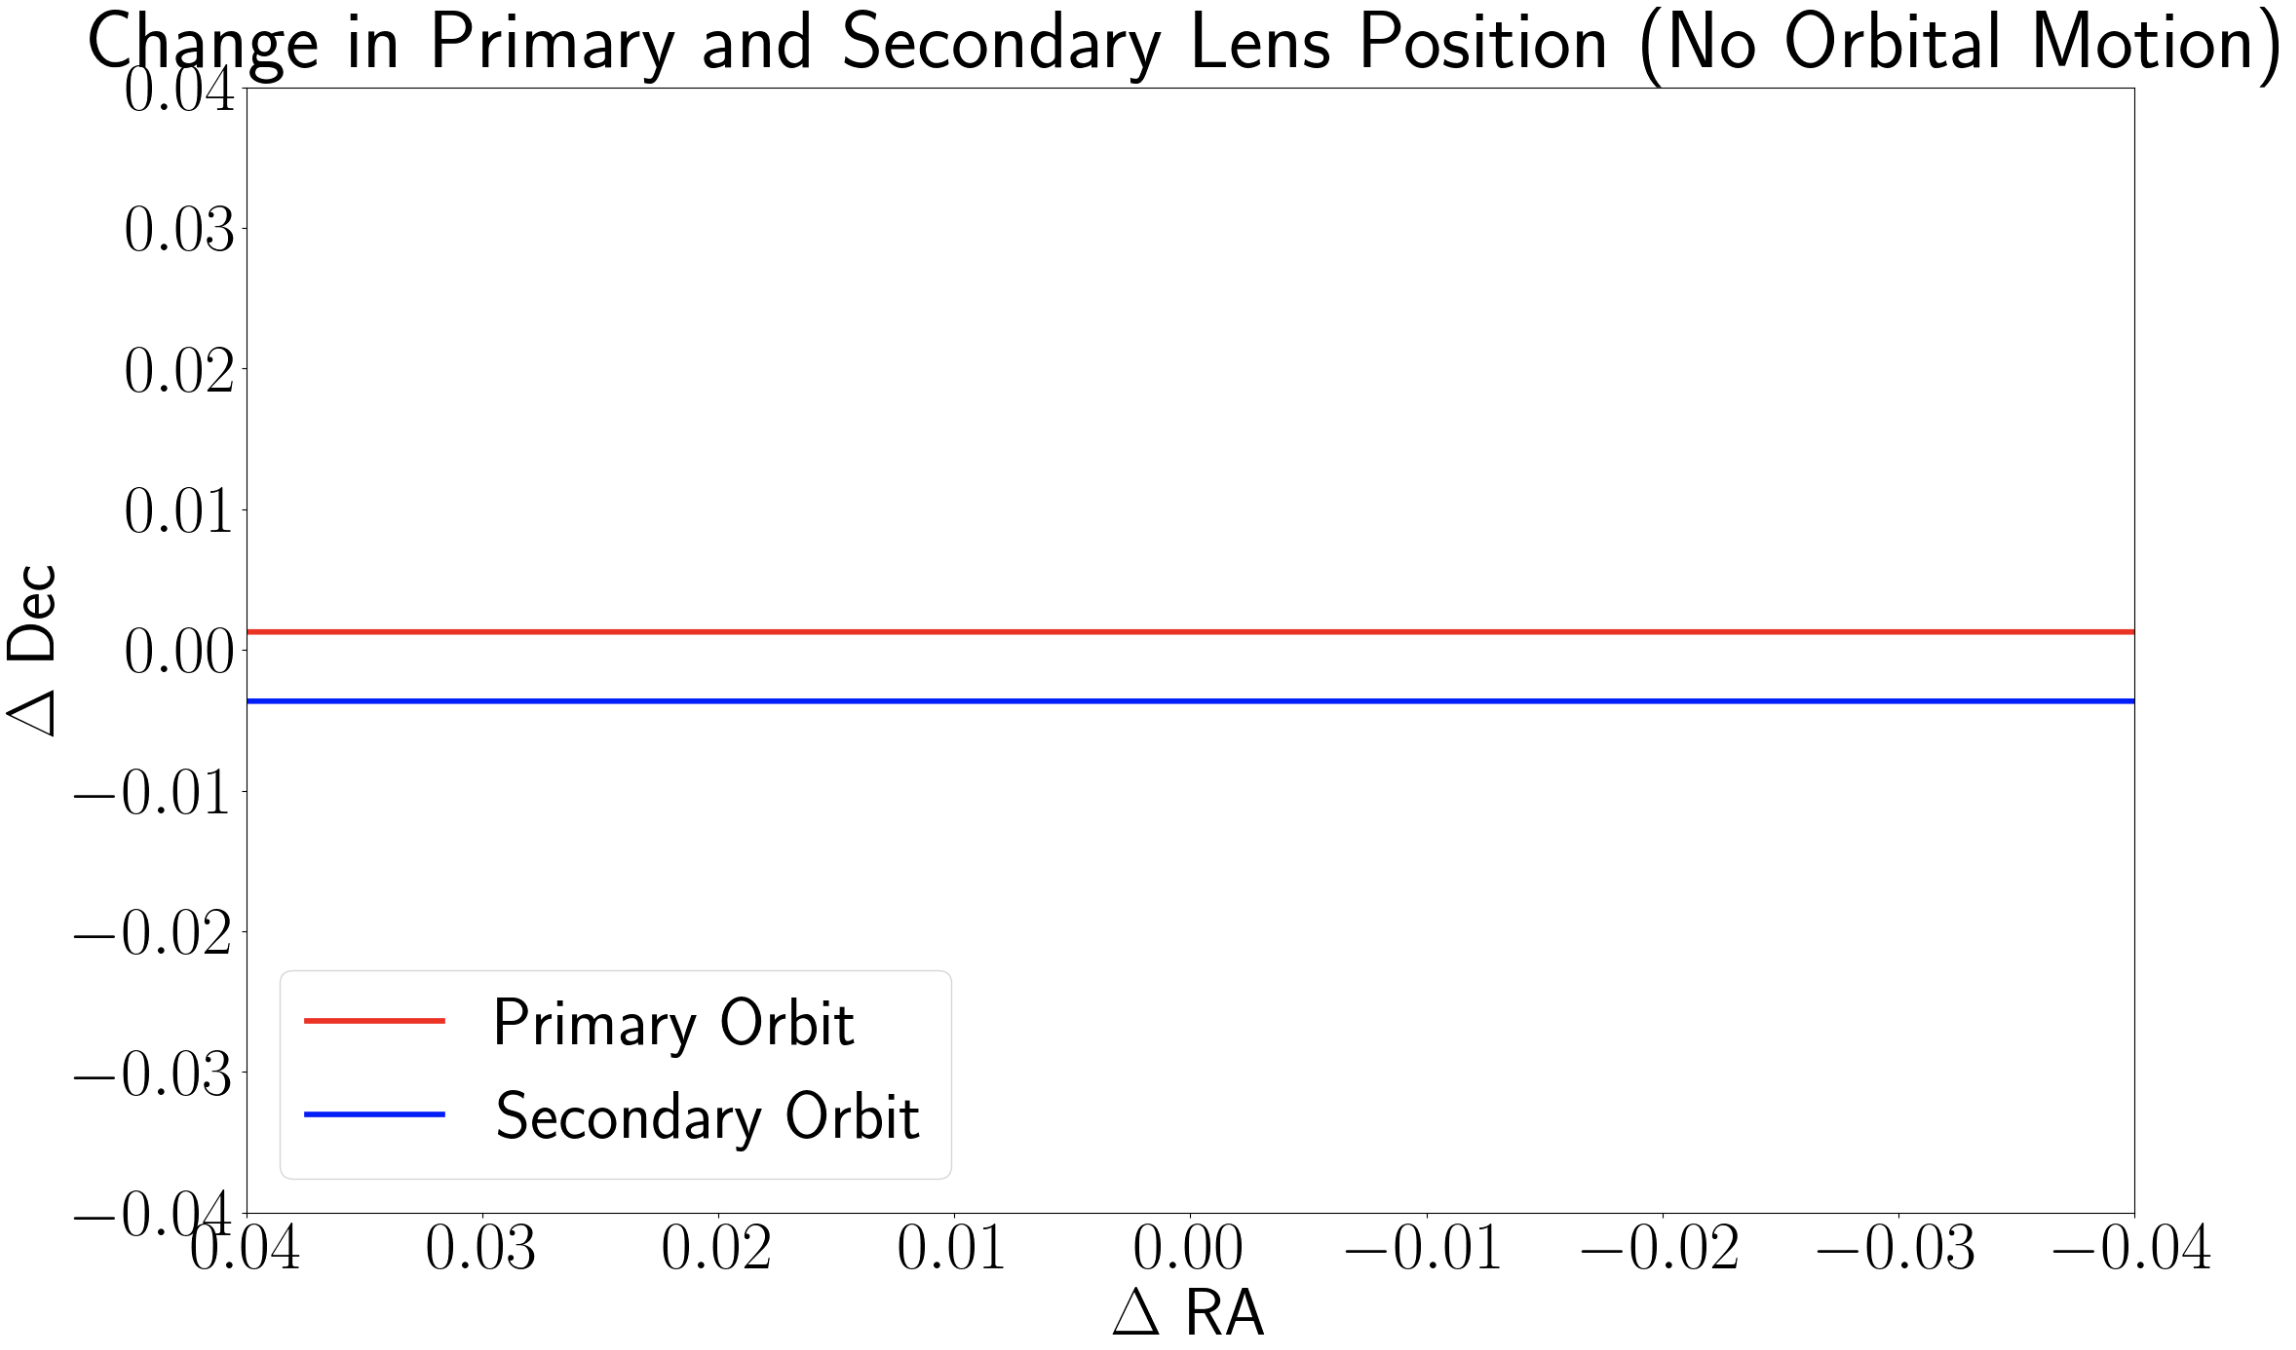
\includegraphics[width=0.5\textwidth]{figures/nomo.png}
    %\caption{Source and lens trajectories for binary objects without orbital motion. We fix the angular separation between the binary objects and propagate them with a proper motion. This simulation provides the primary object with a proper motion of [4 mas yr$^{-1}$, 0 mas yr$^{-1}$] and an angular separation of 5 $mas.$}
   % \label{fig:nomo}
%\end{figure}


%Microlensing models in BAGLE with orbital motion are computationally expensive. For binary orbits with periods much longer than the relevant microlensing timescale $\tE$, including orbital motion may pose unnecessary computational expenses. 

%Thus, while the focus of this paper is reserved for cases in BAGLE with orbital motion, we acknowledge that the simplest case of a binary model in BAGLE involves the binary system moving with a fixed angular separation between them. This works under the assumption that the period of the orbits is much larger than the duration of the microlensing events. 

%Throughout the paper, vector quantities corresponding to the astrometric trajectories of binary objects are decomposed into their RA and Dec components. Since we work only in the Equatorial coordinate system, we also equivalently refer to RA as East and Dec as
%North, subscripted by “E” or “N”, where RA increases
%to the East and Dec increases to the North.

%Thus, in \autoref{fig:nomo}, we present the simulated astrometric paths of a primary and secondary object moving eastwards with a fixed angular separation of 5 $mas$ and a proper motion of [4 mas yr$^{-1}$, 0 mas yr$^{-1}$]. 

\section{Binary Lens Geometries}
\label{sec:binary_geometry}

BAGLE supports binary lens and binary source geometries as shown in different columns of Figure \ref{fig:geometry_binary} for PSBL, BSPL, and BSBL systems.
The simplest case of a binary model in BAGLE involves the binary system moving with a fixed angular separation between the primary and secondary objects. This works under the assumption that the period of the orbits is much larger than the duration of the microlensing. For longer-duration events, the secondary companion moves with respect to the primary.

BAGLE provides models for the secondary companion's motion that is linear, accelerating, or orbiting along a Keplerian trajectory as shown in the different rows of Figure \ref{fig:geometry_binary}. 

\begin{figure}
    \centering
    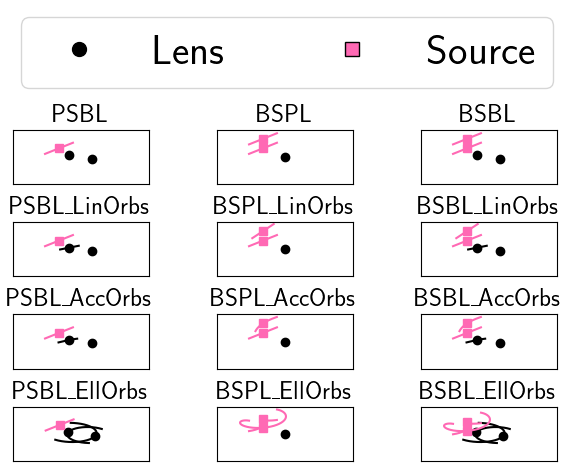
\includegraphics[width= .5 \textwidth]{figures/geometry_schematic_binary_familes.png}
    \caption{Binary geometries available in BAGLE. Models with binary lenses ({\em left column}), binary sources ({\em middle column}), and binary lens and source ({\em right column}) are supported. Secondary companions can have fixed separation and angle relative to the primary ({\em top row}), linear motion ({\em 2nd row}), accelerating motion ({\em 3rd row}), or full Keplerian orbital motion ({\em 4th row}).}
    \label{fig:lens_source_models}
\end{figure}



\section{Binary Orbital Motion in BAGLE \label{sec:binary_solutions}}


\begin{figure*}
    \centering
    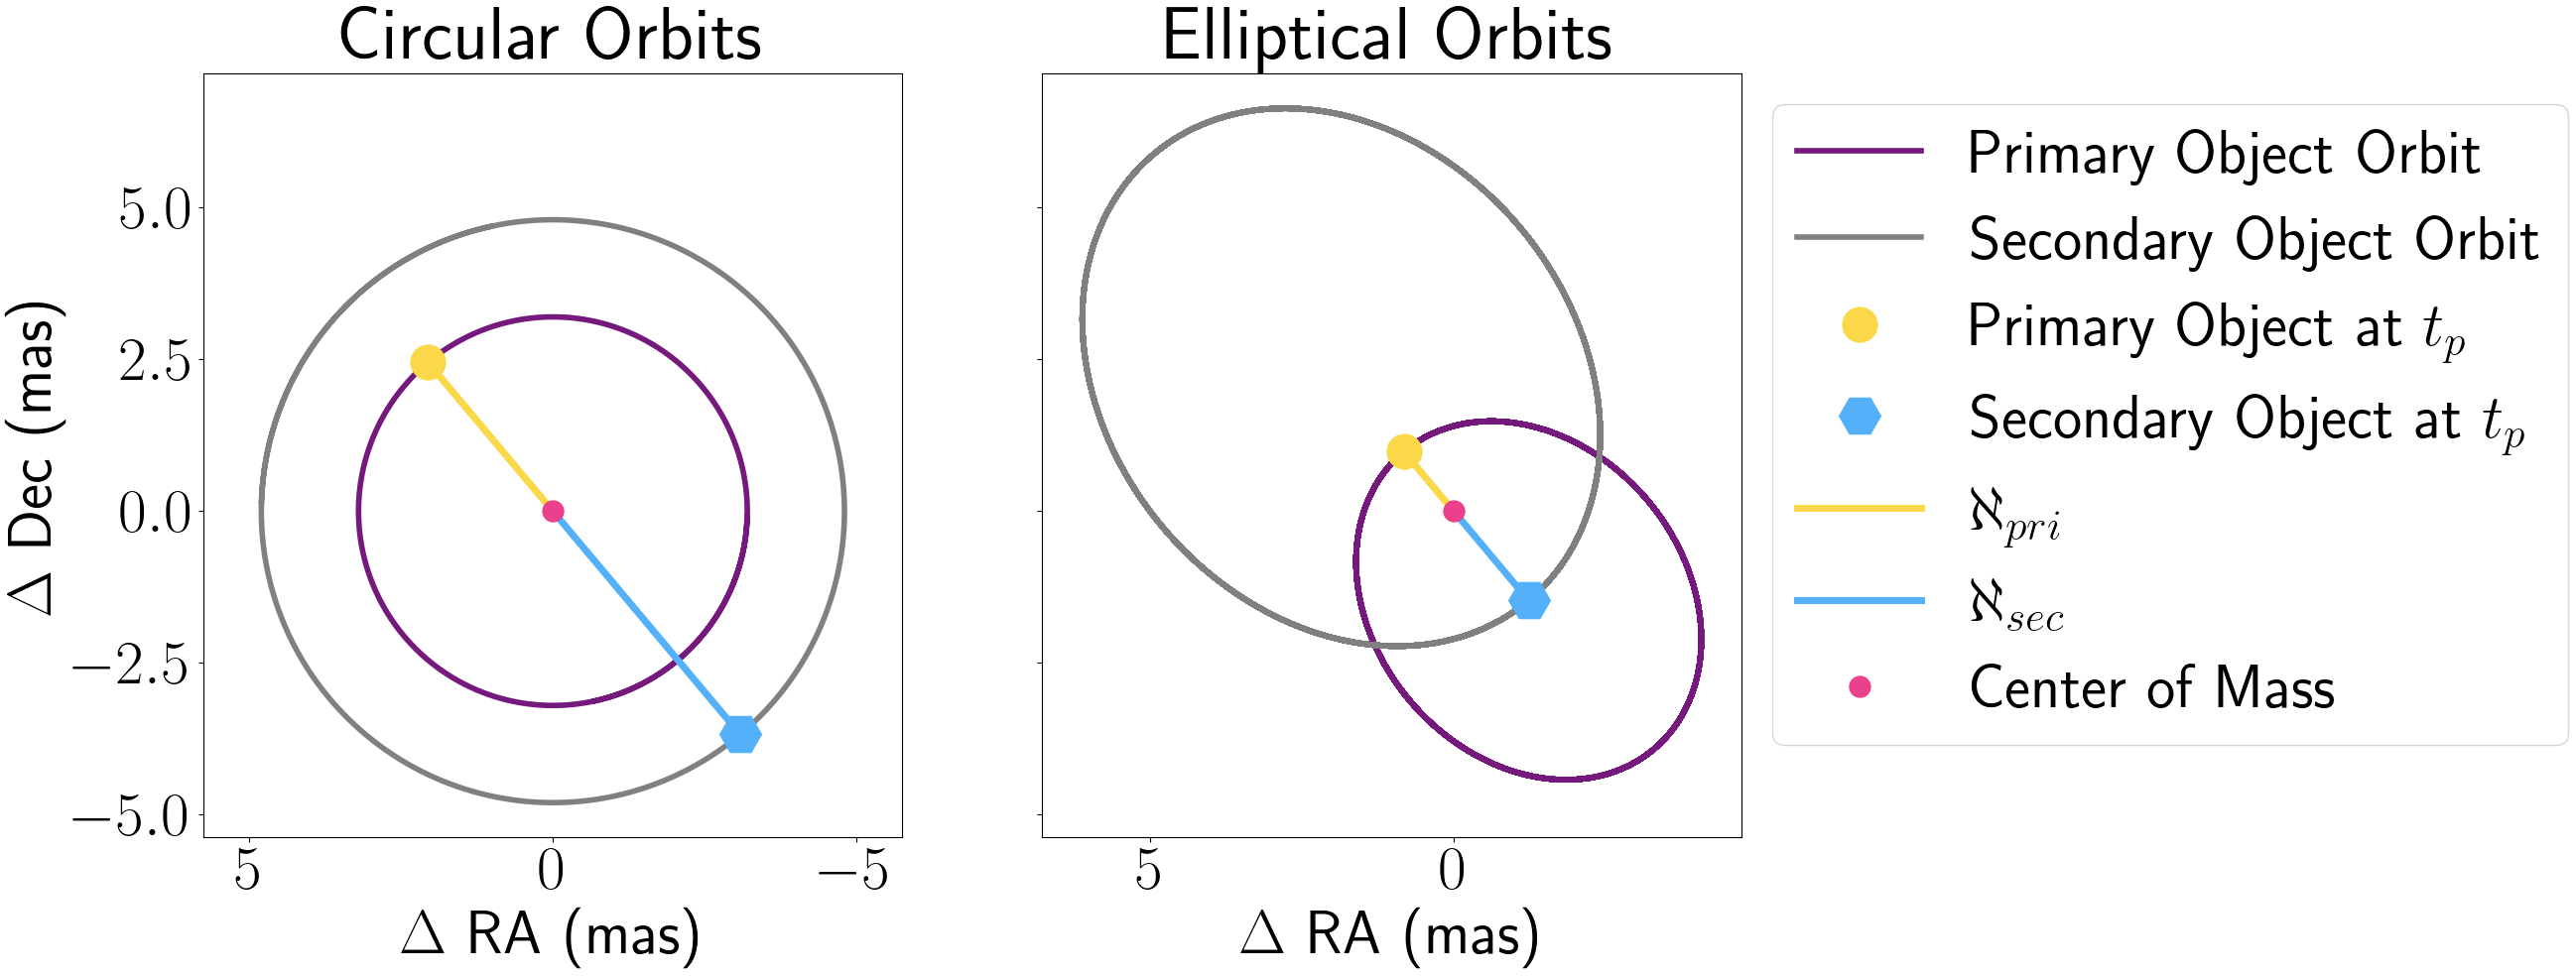
\includegraphics[width=\textwidth]{figures/com_motion.png}
    \caption{Trajectories of binary orbits at $\inclination = 0 \degree$ (binary disk is face-on) simulated using BAGLE for zero center of mass proper motion. The primary and secondary objects at the time of periastron passage have been highlighted on both plots. (\emph{Left}) A circular orbit. (\emph{Right}) An elliptical orbit with an eccentricity of $0.6$. }
    \label{fig:com_geometry}
\end{figure*}



BAGLE is capable of modeling microlensing events using physical parameters such as the mass of the lens, the distance to the lens, flux, sky position, and proper motion of the lens and the source star. In order to support binary companions to the lens, the source, or both, we introduce many new parameters to describe the mass ratios, flux ratios, and orbital parameters for each binary system. 

To model the primary and secondary motion around the center of mass, the following Keplerian orbital parameters are used: 

%The dynamics of any binary system involve two gravitationally bound celestial objects moving around a common center of mass in eccentric orbits. As demonstrated in \citep{Lu:2025}, BAGLE includes photometric and astrometric parameters. To implement orbital motion in BAGLE, we now input Keplerian elements as well. 

%For each respective model with orbital motion, we maintain consistency in our definition of $\tnot$ with the case where no orbital motion is considered. We explore our definition of $\tnot$ and the associated coordinate conversions in detail when discussing the nature of our binary sources (i.e., binary lenses or sources) in later sections of this document.

\begin{itemize}
\label{keplerian_elems}
    \item $\w$: The argument of periastron of the primary object's orbit in degrees. The secondary companion is placed $180 \degree$ across the primary's argument of periastron. 
    \item $\inclination$: Inclination angle of the system in degrees. The primary and secondary objects share the same inclination angle.  An inclination of $0\degree$ means that the system is face-on.
    \item $\bigomega$: The longitude of the ascending node of the secondary companion's orbit in degrees. 
    \item $\eccentricity$: Eccentricity of the Keplerian orbit. For circular orbits, this is fixed to 0. 
    \item $\period$: The orbital period of the binary system in days. 
    \item $t_p$: The time of the periastron of the system in days. 
    \item $\al$: The semi-major axis of the primary object in mas.
    \item $\ala$: The semi-major axis of the secondary object in mas. 
\end{itemize}

Note that not all of the Keplerian elements are required as inputs to BAGLE models. Depending on the nature of the binary object (i.e., whether it is a binary source or a lens) and the parameterization used, the input microlensing parameters vary. The center of mass of the binary system is located at the point where the binary orbit intersects the reference plane in the sky.
The reference direction is the North direction in the plane-of-sky. Hence, $\bigomega$ is recorded Eastward of North, and $\w$ is Eastward of $\bigomega + 180 \degree$. 

In BAGLE, the eight Keplerian elements presented above are used to estimate the Thiele-Innes constants as described in \citet{Koren_2016} and presented, in detail, in Appendix \ref{sec:Thiele-Innes}. Using these constants, the positions of the primary and the secondary companion over time are computed. Let  $\Xcomp$ be the primary object's trajectory around the center of mass, with $\Xcomep$ and  $\Xcomnp$ being the East and North components, respectively. Let  $\Xcoms$ be the secondary companion's trajectory around the center of mass with $\Xcomes$ and  $\Xcomns$ representing the East and North components, respectively. Then, the following set of equations holds: 



%\subsection{Calculating Orbital Solutions with Keplerian Elements}

%Once we determine the Keplerian elements of a binary orbit, we can obtain the trajectory of the involved celestial objects around their common center of mass. Our method for calculating these trajectories was introduced in \citet{Koren_2016}.


%With the Thiele-Innes constants, plus rectangular coordinates defined, we can now define the primary and secondary orbital trajectories. 

%We now present equations necessary to model the movement of binary objects around their center of mass.

%Let  $\Xcomp$ be the primary object's trajectory around the center of mass in the heliocentric frame, with $\Xcomep$ and  $\Xcomnp$ being the East and North components, respectively. Let  $\Xcoms$ be the secondary object's trajectory around the center of mass with $\Xcomes$ and  $\Xcomns$ representing the East and North components, respectively. Then, the following set of equations holds true: 
\begin{eqnarray}
\label{eqn:tinnes}
    \Xcomep &= X(t) \Bpri + Y(t) \Gpri  \nonumber \\
    \Xcomnp &= X(t) \Apri + Y(t) \Fpri  \nonumber \\
    \Xcomes &= X(t) \Bsec + Y(t) \Gsec \nonumber \\
    \Xcomns &= X(t) \Asec + Y(t) \Fsec 
\end{eqnarray}
%We can now simulate the orbital trajectories in BAGLE as:
%\begin{align}
 %   \label{eqn:pri_om}
  %  \Xcomp = \left[ \Xcomep, \Xcomnp \right] \\
   %     \label{eqn:sec_om}
    %\Xcoms = \left[ \Xcomes, \Xcomns \right] 
%\end{align}
where $X(t)$ and $Y(t)$ are the rectangular coordinates of the binary system; $A_{pri}$, $A_{sec}$, $B_{pri}$, $B_{sec}$, $G_{pri}$, $G_{sec}$, $F_{pri}$ and $F_{sec}$ are the Thiele-Innes constants. 

Using Eqn~\ref{eqn:tinnes}, BAGLE can model circular and elliptical orbital trajectories around the center of mass, as shown in Figure~\ref{fig:com_geometry}. Note that the equations in this section describe the motion around the center of mass. The proper motion of the center of mass in the observer's frame of reference is accounted for separately. 

%However, the dynamics of binary orbits for microlensing events are not limited to their orbital motion around a center of mass. The center of mass can have a proper motion in the observer's frame of reference. 


\section{Binary Sources and Point Lenses (BSPL) \label{sec:binsource}}

In this section, we will discuss microlensing models for binary sources. We begin by discussing simple, static approximations in \S\ref{sec:binsources_static}. Then, we expand to a discussion of linear and accelerated orbital approximations in \S\ref{sec:binsources_lin}. Finally, the full Keplerian solutions are presented in \S\ref{sec:binsources_kep}, followed by a discussion of microlensing equations in \S\ref{sec:binsources_eqn}.

\subsection{Static Approximation}
\label{sec:binsources_static}

In binary-source models, the components of the binary (i.e., the primary source and the secondary source companion) are initially at rest relative to each other. On the plane of the sky, in the SSB frame, at $\tnot$, the binary source system initially has a fixed angular separation of:

\begin{equation}
    \vect{s}(\tnot) = \Xssvec(\tnot) - \Xspvec(\tnot)
\end{equation}
%
where $\vect{s}(\tnot)$ is the separation vector at $\tnot$, $\Xssvec(\tnot)$ is the initial secondary source position on the sky at $\tnot$, and $\Xspvec (\tnot)$ is the initial primary source position on the sky at $\tnot$. In the binary-source models, $\tnot = \tpnot$, i.e., $\tnot$ is the time of closest approach between the primary source and the lens ($\tpnot$). The angular separation between the primary and the secondary companion is fixed at all times. The proper motion of the secondary companion is assumed to be the same as the proper motion of the primary source. 

\subsection{Linear and Accelerated Orbital Approximations}
\label{sec:binsources_lin}

\begin{figure}
    \centering
    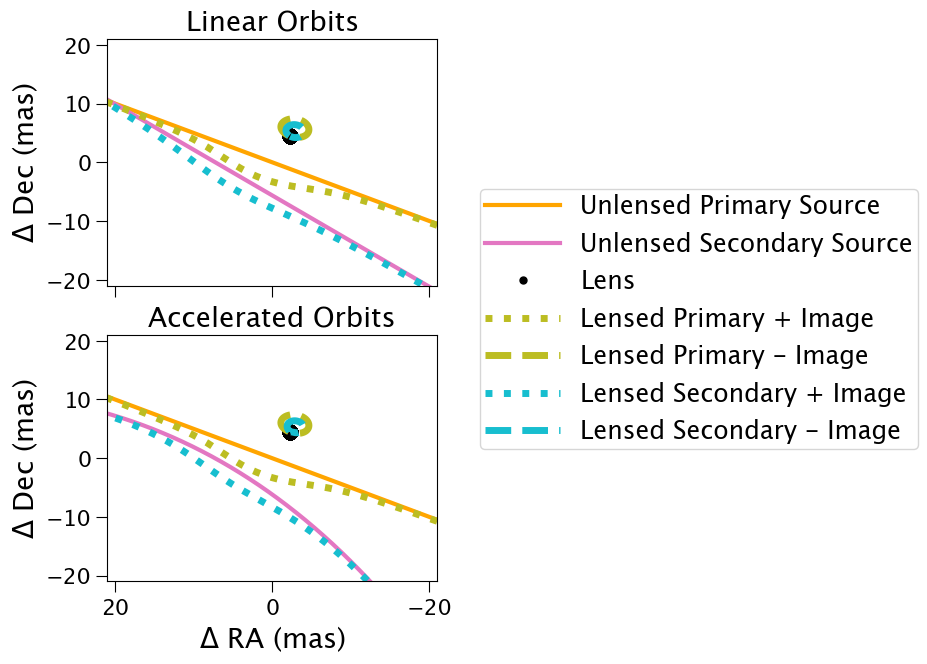
\includegraphics[width=0.5\textwidth]{figures/linorbs.png}
    %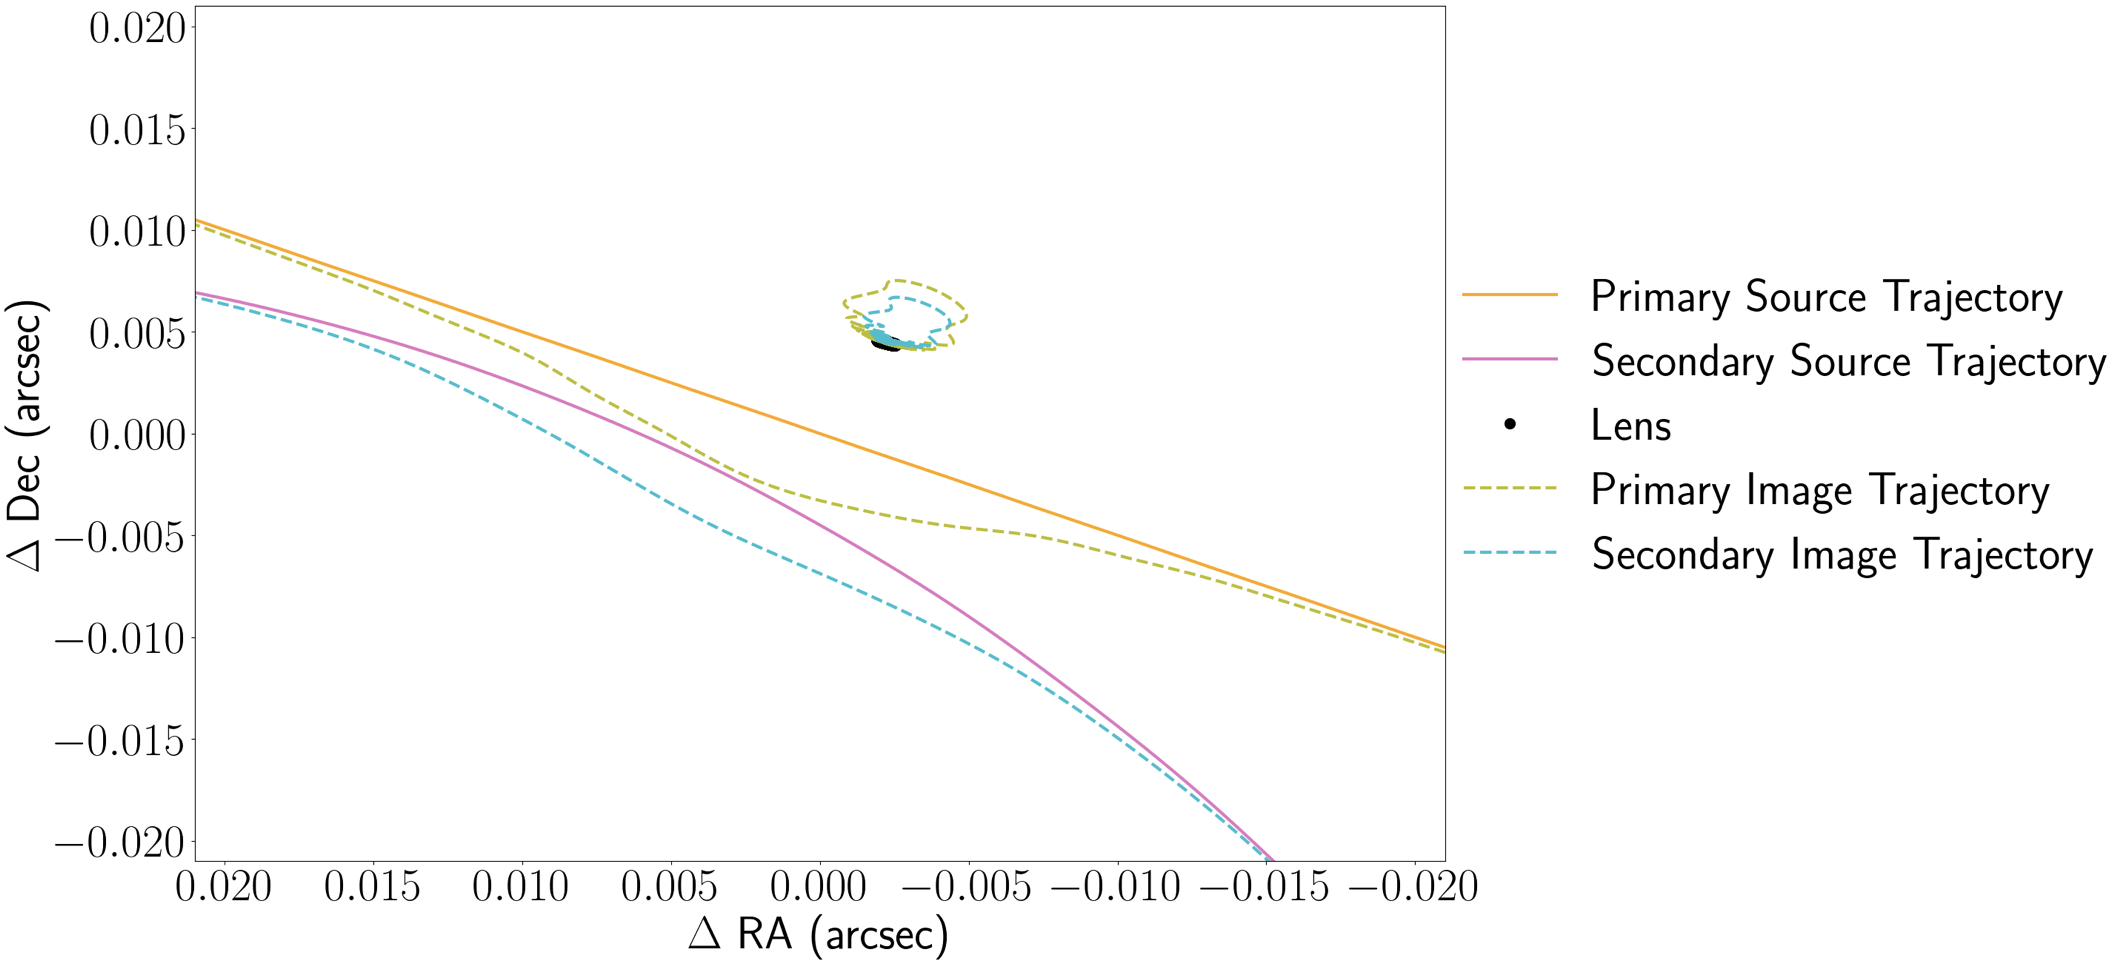
\includegraphics[width=0.48\textwidth]{figures/accorbs.png}
    \caption{Source and lens trajectories for linear (\emph{Top}) and accelerated (\emph{Bottom}) approximations of orbital motion in binary sources. We present the unlensed sources (solid lines) and the lensed images (dashed + dotted lines). For each source, there is a major and a minor image. The minor image is seen around the lens, and the major image is seen around the source. In both panels, the primary's proper source motion $\musvec$ is [6 mas yr$^{-1}$, 3 mas yr$^{-1}$]; the secondary's proper source motion relative to the primary source $\mussvec$ is [9 mas yr$^{-1}$, 7 mas yr$^{-1}$]. The acceleration of the secondary source $\accSsec$ is [0.5  mas yr$^{-2}$, -2  mas yr$^{-2}$] in the lower panel. In both cases, the Einstein time ($\tE$)=269 days and $\uo$ =1.01 $\thetaE$. The lens mass is $10 M_\odot$, and it is held stationary.}
    
    \label{fig:bspl_linacc}
\end{figure}

In contrast to the static approximation, in both the linear and accelerated orbit models, the primary and the secondary companion move with different proper motions. 

For linear approximations, BAGLE inputs a new parameter $\deltamussvec$, which is the proper motion of the secondary source relative to the primary source. With time, due to the proper motion of the primary and secondary sources, the separation vector $\vect{s(t)}$ between the sources changes. The secondary source moves linearly relative to the primary source. The positions of the primary and secondary sources are given by:

\begin{align}
    \Xspvec (t) = & \Xspovec + \musvec [t - \tnot] \nonumber \\
    &+\pi_S \vect{P}(t, \alpha, \delta)  
    \label{linear_motion}    
\end{align}


\begin{align}
    \Xssvec (t) = & \Xssovec + \mussvec [t - \tnot ]\nonumber \\
    &+\pi_S \vect{P}(t, \alpha, \delta)  
    \label{linear_motion2}    
\end{align}
%
where $\musvec$ is the proper motion of the primary source, and $\mussvec$ is the proper motion of the secondary source calculated as $\mussvec = \musvec + \deltamussvec$. Furthermore, we account for the parallactic motion at time $t$ in the direction of the source-lens system $(\alpha, \delta)$, given by the difference of the Earth and Sun's position, normalized by 1 AU.  The parallactic motion is $\pi_S
\vect{P}(t, \alpha, \delta)$ where $\pi_S$ is the
maximum parallax amplitude $1/d_S$ and $\vect{P}(t, \alpha, \delta)$ is the actual parallax direction and fractional amplitude on the sky.

For accelerated approximations, along with $\deltamussvec$, BAGLE also inputs $\accSsec$, which is the acceleration of the secondary source relative to the lens. In the accelerated orbit model, the secondary source moves with constant acceleration relative to the primary source. The positions of the primary and secondary sources are given by: 




\begin{align}
    \Xspvec (t) = & \Xspovec + \musvec [t - \tpnot] \nonumber + \\
    &+\pi_S \vect{P}(t, \alpha, \delta)  
    \label{accelerated motion}    
\end{align}


\begin{align}
    \Xssvec (t) = & \Xssovec + \mussvec [t - \tpnot ]\nonumber \\
    &+\frac{1}{2}\accSsec[t - \tpnot]^2 +\pi_S \vect{P}(t, \alpha, \delta)  
    \label{accelerated_motion2}    
\end{align}
%

An example of the linear and accelerated orbital approximations is presented in Figure~\ref{fig:bspl_linacc}, showing the change in Right Ascension ($\Delta \alpha^*$) and Declination ($\Delta \sigma$) of the primary source (lensed and unlensed), secondary source (lensed and unlensed), and the lens. The lensed images are further categorized into the major (``+") image and minor (``-") image. These figures can be generated using BAGLE with the code lines below. For this example, we use \texttt{BSPL\_PhotAstrom\_noPar\_LinOrbs\_Param2}, which is a model for linear orbits. One can follow the same steps below to generate plots for accelerated orbits:

\begin{lstlisting}[language=Python]
from bagle import model

#Create a linear orbital model with photometric and astrometric parameters

bsplorbits = model.BSPL_PhotAstrom_noPar_LinOrbs_Param2(
                 t0, u0_amp, tE, thetaE,
                 piS, piE_E, piE_N,
                 xS0_E, xS0_N,
                 muS_E, muS_N,
                 delta_muS_sec_E, 
                 delta_muS_sec_N,
                 sep, alpha, fratio_bin,
                 mag_base, b_sff, dmag_Lp_Ls,
                 raL=None, decL=None)
                 
# Get resolved astrometry for unlensed source positions
t_obs = np.arange(t0 - 10*tE, t0 + 10*tE, 1)
bsplorbits.get_resolved_source_astrometry_unlensed(t)
srce_pos_primary =xS_unlensed[:, 0, :]
srce_pos_secondary = xS_unlensed[:, 1, :] 

# Get lens astrometry
lens = bsplorbits.get_lens_astrometry(t)

# Get unresolved astrometry for lensed source positions
xS_lensed = bsplorbits.get_astrometry_shift(t)
lensed_pos_pri = xS_lensed[:, 0, :]
lensed_pos_sec =  xS_lensed[:, 1, :]

#Plot
plt.plot(lens[:, 0], lens[:, 1])
plt.plot(srce_pos_primary[:, 0], srce_pos_primary[:, 1])
plt.plot(srce_pos_secondary[:, 0], srce_pos_secondary[:, 1])
plt.plot(lensed_pos_pri[:, 0], lensed_pos_pri[:, 1])
plt.plot(lensed_pos_pri[:, 0], lensed_pos_pri[:, 1])

\end{lstlisting}


Note that BAGLE has other parameterizations for both linear and accelerated orbits that can be instantiated with different microlensing parameters (e.g., source magnitude instead of baseline magnitude).


%In \autoref{fig:astrometric_shifts}, we observe the lens-induced astrometric shift from the combined centroid motion of the primary and secondary source (bottom-left). We observe that linear and accelerated orbits can significantly affect the astrometric shift over time. Both plots below (bottom-left and bottom-right) account for parallax effects. In \autoref{fig:centroid_shifts}, the centroid shift (bottom-right) is plotted in RA and Dec with source proper motion subtracted. Compared to the case with no orbits, linear and accelerated orbits are more wobbly since the separation between the two sources changes with respect to time.



\subsection{Full Keplerian Solutions}
\label{sec:binsources_kep}
\begin{figure*}
    \centering
    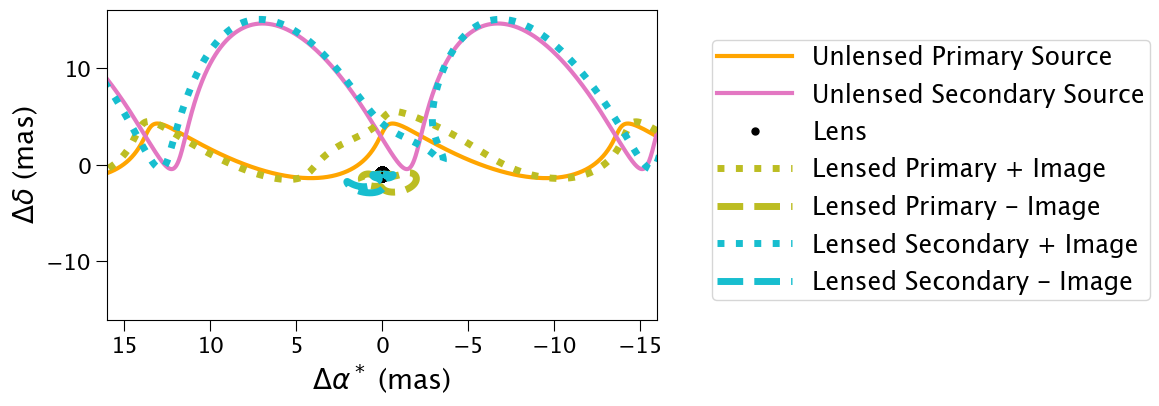
\includegraphics[width=  \textwidth] {figures/bspl_keplerian.png}
    \caption{Source and lens trajectories for a simulated binary source point lens microlensing event involving Keplerian orbits. We present the unlensed sources (solid lines) and the lensed images (dashed + dotted lines). This event has the following Keplerian elements: $\w = 30 \degree$, $\bigomega = 10 \degree$, $\inclination = 90 \degree$, $e=0.6$, $\period = 1000$ days, $\al = 3  $~mas and $\ala = 8 $ mas. We simulate this event over $t_E=208.47$ days. The lens (8 $M_\odot$) is held stationary.}
    \label{fig:bspl_keplerian}
\end{figure*}

All binary-source models with  Keplerian motion in BAGLE input the following Keplerian orbital parameters: $\w$, $\inclination$, $\bigomega$, $\eccentricity$ (for elliptical orbits only), $\period$, $t_p$, $\al$, $\ala$. These models input an additional quantity $\mussysvec$, which is the proper motion of the source system's center of mass in the observer's frame of reference. $\Xscomvec$ is the position of the binary source's center of mass at $\tnot=\tpnot$. While BAGLE inputs $\tnot = \tpnot$ as the time of closest approach between the primary source and the lens, and $\uo$ as the closest approach between the primary source and the lens, it can convert between different coordinate systems (e.g., to use the closest approach between the source system center of mass and the lens). Conversions for
$\tnot$ and $\uo$ are presented in Appendix \ref{sec:u0} and \ref{sec:t0}.

%We can convert $\tnot$ to $\tcomnot$, which is the time of closest approach between the source system's center of mass and the lens. We can also convert $\uo$ to $\uocom$, which is the closest approach between the source system's center of mass and the lens. We cover these coordinate conversions in the Appendix.

%Using the period of the source, the semi-major axis of the primary and secondary sourced, and Kepler's law, we calculate the mass ratio of the sources to find $q=\frac{M_{source, primary}}{M_{source, sec}}$ and $q' = \frac{1-q}{1+q}$. Additionally, we use $\al$ and $\ala$ to find the initial separation of the sources as $sep = \al + \ala$. The dimensionless separation between the sources can be denoted by expressing $sep$ as a fraction of $\thetaE$: $s = \frac{sep}{\thetaE}$. Now we complete the coordinate conversion from $\tpnot$  to $\tcomnot$:

%\begin{eqnarray}
 %  \tcomnot = \tpnot + s t_E cos(\phi)\left(q'-\frac{1}{2}\right)
%end{eqnarray}

In Figure~\ref{fig:com_geometry}, we demonstrated the motion of the primary and its secondary companion around the center of mass at rest. After accounting for the proper motion of the center of mass, the primary and secondary source trajectories (including parallactic motion) are given by: 

%we propagate the source's center of mass with its proper motion. Thus, we internally switch from the initial position of the primary source $\Xsovec$ to $\Xscomvec$, which is defined as the initial position of the binary source system's center of mass at $\tnot = \tpnot$. 


\begin{align}
    \Xspvec =& \Xscomvec + \mussysvec  [t - \tpnot] \nonumber \\
    +& \Xcomp + \pi_S \vect{P}(t, \alpha, \delta) \\
    \Xssvec =& \Xscomvec + \mussysvec [t - \tpnot] \nonumber \\
    +& \Xcoms + \pi_S \vect{P}(t, \alpha, \delta) 
\end{align}

We simulate a binary microlensing event to see the effects of complete Keplerian orbital motion in Figure~\ref{fig:bspl_keplerian}. 

\subsection{Lensing a binary source}
\label{sec:binsources_eqn}

The equations of relative separation between each source and lens, in units of Einstein radii, are
\begin{eqnarray}
\upveco &= \frac{\Xspvec-\Xlvec}{\thetaE} \\
\usveco &= \frac{\Xssvec-\Xlvec}{\thetaE} \\
\end{eqnarray}
in the heliocentric frame.

If the lensing event could be fully resolved, we would expect to see four lensed images, two for each source. 

The amplifications for the images are
\begin{eqnarray}
A_{p,\pm} &= \frac{1}{2} \left( 1 \pm \frac{\upvec^2 + 2}{\upvec \sqrt{\upveco^2 + 4}} \right) \\
A_{s,\pm} &= \frac{1}{2} \left( 1 \pm \frac{\usvec^2 + 2}{\usvec \sqrt{\usvec^2 + 4}} \right) 
\end{eqnarray}
where the two images per source are labeled $+$ for the major image and $-$ for the minor image.


Each source's intrinsic flux is magnified by its specific amplification factors. The total amplification for each source is
\begin{eqnarray}
 A_p &= \frac{\upvec^2 + 2}{\upvec \sqrt{\upvec^2 + 4}} \\
 A_s &= \frac{\usvec^2 + 2}{\usvec \sqrt{\usvec^2 + 4}}
\end{eqnarray}

We can define a total amplification for the system using
\begin{eqnarray}
 A = \frac{A_p f_p + A_s f_s}{f_p + f_s}
\end{eqnarray}
where $f_p$ and $f_s$ are the intrinsic flux of the primary and secondary sources.

The observed flux for the lensed system is then
\begin{eqnarray}
f_{obs} = (A_p f_p + A_s f_s) \left(1 + \frac{1 - \bsff}{\bsff} \right).
\end{eqnarray}
% (avoiding indent for a continued sentence)
where $\bsff$ is the ratio of the source flux to the total flux of the source, neighbors, and the lens.  

The lensed astrometry, or the image centroid, ($\XIvec$) is then simply a flux-weighted combination of the lensed astrometry from the two sources:

\begin{eqnarray}
    \XIvec = \frac{\Xspvec A_p f_p + \Xssvec A_s f_s}{f_p+f_s}
\end{eqnarray}


\section{Point Sources and Binary Lens (PSBL) 
\label{sec:binlenses}}



In this section, we begin by discussing the static lens approximation in \S\ref{sec:binlenses_static}, followed by the linear and accelerated orbital approximations in \S\ref{sec:binlenses_lin}. In \S\ref{sec:binlenses_kep}, the full Keplerian solutions are presented. Lastly, we discuss the microlensing equations for bianry lenses in \S\ref{sec:binlenses_eqn2}.

\subsection{Static Approximation}
\label{sec:binlenses_static}

Like binary source models in BAGLE, the simplest implementation of a PSBL model in BAGLE fixes the angular separation between the primary and secondary lens at all times. The two lenses are separated by an initial separation given in Equation~\ref{eqn:sep}.

\begin{equation}
    \label{eqn:sep}
    \vect{s}(\tnot) = \Xlsvec(\tnot) - \Xlpvec(\tnot)
\end{equation}

For binary lenses, $\tnot=t_{geo, 0, \sun}$ in static, linear and accelerated orbital approximations. $t_{geo, 0, \sun}$ represents the time of closest approach between the source and the geometric midpoint of the binary lenses. In the static approximation only, the angular separation between the primary and secondary lens is fixed at all times; both lenses move with the same proper motion vector. 

\subsection{Linear and Accelerated Orbital Approximations}
\label{sec:binlenses_lin}


\begin{figure}
    \centering
    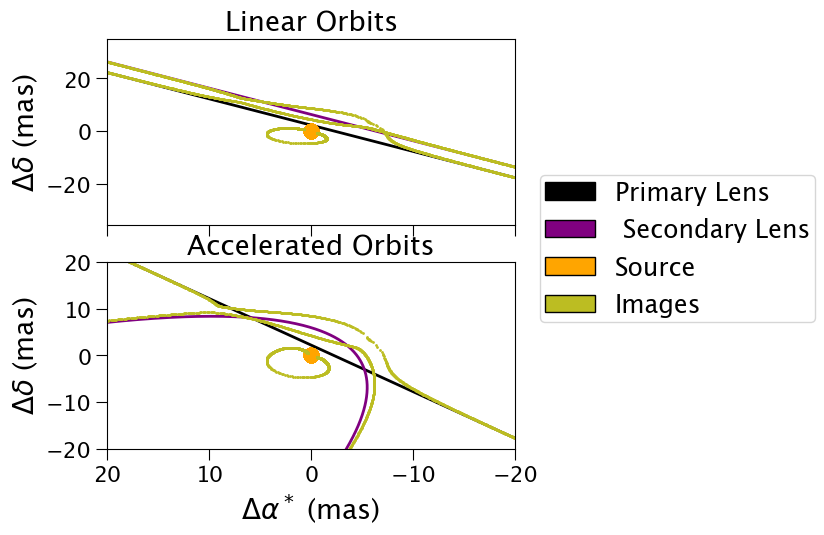
\includegraphics[width=0.5\textwidth]{figures/lin_lenses.png}
    %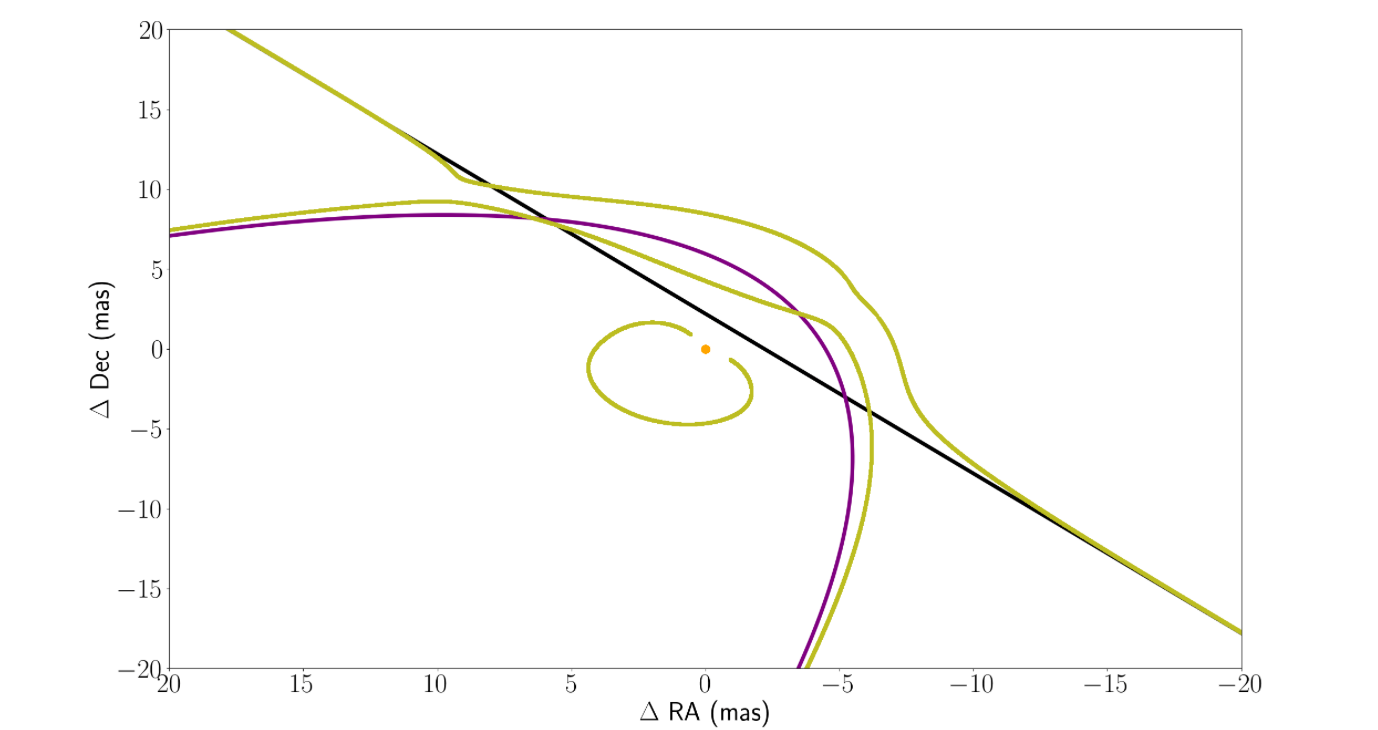
\includegraphics[width=0.5\textwidth]{figures/acc_lenses.png}
    \caption{Source and lens trajectories for linear (upper panel) and accelerated (lower panel) approximations of orbital motion of binary lenses. The solid black line is the primary lens, the solid purple line is the secondary lens, and the solid yellow lines are the image positions. In both panels, the source is stationary; the primary lens has a proper motion of $\mulvec$ = [-3.76 mas yr$^{-1}$, -3.76 mas yr$^{-1}$]; the secondary lens has a proper motion of  $\mulsvec$ = [-2.76 mas yr$^{-1}$, -2.76 mas yr$^{-1}$]. For our model with acceleration, we provide the following input for $\accLsec$ = [1 mas yr$^{-1}$, -1 mas yr$^{-1}$]. In both cases, the Einstein time ($\tE$)=412 days and $\uo$ = 0.5 $\thetaE$. Note that this scenario does not involve a caustic crossing and thus produces only 3 images.}
    \label{fig:psbl_linacc}
\end{figure}


%For binary lens systems with a long period, performing a fit using linear or accelerated approximations is computationally favorable. While these trajectories are physically not representative of the true orbit, they can serve as effective close approximations. 

%Like binary source models in BAGLE, the simplest implementation of a PSBL model in BAGLE fixes the angular separation between the primary and secondary lens at all times. The two lenses are separated by an initial separation given in Equation~\ref{eqn:sep}

%\begin{equation}
 %   \label{eqn:sep}
  %  \vect{s}(\tnot) = \Xlsvec(\tnot) - \Xlpvec(\tnot)
%\end{equation}

The linear orbital approximations for binary lenses follow the same logic as binary sources in Sec.~\ref{sec:binsources_lin}. Therefore, after accounting for parallactic motion (given by $\pi_L
\vect{P}(t, \alpha, \delta)$ where $\pi_L$ is the
maximum parallax amplitude of the lens, $1/d_L$), the positions of the primary and secondary lenses are given by: 

\begin{eqnarray}
\label{linear_motion}
    \Xlpvec (t) =& \Xlpovec + \mulvec [t - t_{geo, 0, \sun}] \nonumber \\
    +& \pi_L \vect{P}(t, \alpha, \delta) \\
\label{linear_motion2}
    \Xlsvec (t) =& \Xlsovec + \mulsvec [t - t_{geo, 0, \sun}]   \nonumber \\
    +&  \pi_L \vect{P}(t, \alpha, \delta) 
\end{eqnarray}
%
where $\mulvec$ is the proper motion of the primary lens and $\mulsvec$ is the proper motion of the secondary lens. PSBL models with linear orbital approximations input a new parameter $\deltamulsvec = \mulsvec - \mulvec$, which is the proper motion of the secondary lens relative to the primary.

For accelerated approximations, BAGLE takes in $\deltamulsvec$ and another new parameter  ($\accLsec$), which is now the acceleration of the secondary lens relative to the primary lens. The positions of the primary and secondary lenses are given by: 

\begin{align}
\label{accelerated_motion}
    \Xlpvec (t) =& \Xlpovec + \mulvec [t - t_{geo, 0, \sun}] \nonumber \\
    +& \pi_L \vect{P}(t, \alpha, \delta) \\
\label{linear_motion2}
    \Xlsvec (t) =& \Xlsovec + \mulsvec [t - t_{geo, 0, \sun}]   \nonumber \\
    +& \frac{1}{2}\accLsec[t - \tpnot]^2 +  \pi_L \vect{P}(t, \alpha, \delta) 
\end{align}

We present examples for linear and accelerated orbital approximations involving binary lenses in Figure~\ref{fig:psbl_linacc}.

\subsection{Full Keplerian Solutions}
\label{sec:binlenses_kep}


\begin{figure}
    \centering
    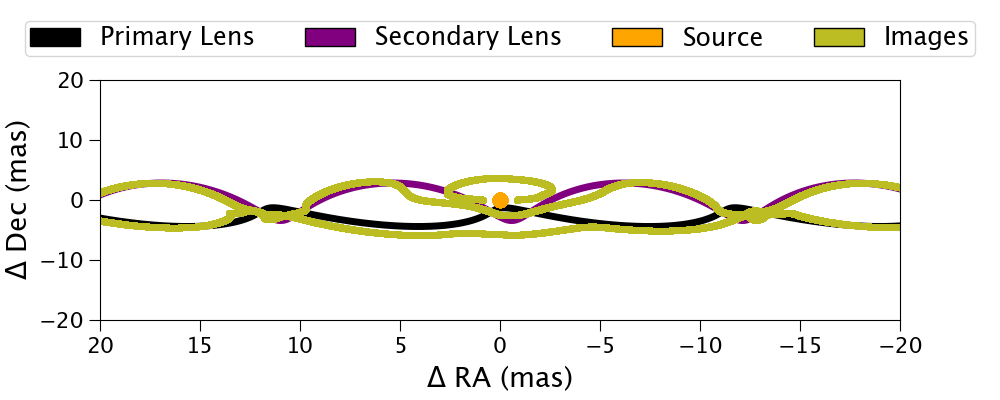
\includegraphics[width= .5 \textwidth] {figures/psbl_keplerian.png}
    \caption{Source and lens trajectories for a simulated microlensing event with a binary lens. The solid black line is the primary lens, the solid purple line is the secondary lens, the orange point is the source position, and the solid yellow lines are the image positions. We use the following orbital parameters: $\w = 30 \degree$, $\bigomega = 10 \degree$, $\inclination = 90 \degree$, $e=0.6$, $\period = 1054.41 $ days, and an angular separation of $5$ mas between the two lenses at $\tcomnot$. We present our simulation over $t_E=412.02$ days. The lenses have a mass of $m_{L,p}=$ 10 $M_\odot$ and $m_{L,s}=$ 5 $M_\odot$. The source is stationary.}
    \label{fig:psbl_keplerian}
\end{figure}

All binary-lens models with Keplerian orbital motion (either circular or elliptical) input the following new Keplerian elements: $\w$, $\bigomega$, $\inclination$, $\eccentricity$, $t_p$, and $a$, where $a$ is the magnitude of the semi-major axis in angular units (mas) at $t_p$. We can convert $a$ to the semi-major axis in units of AU ($a_{AU}$) by using $a$ and the distance to the lens ($d_L$) in units of pc, i.e., $a_{AU} = a \times d_L$. In these models, $\mulvec$ is treated as the proper motion of the binary lens system's center of mass instead of the geometric midpoint of the binary lens. As such, we change the notation from $\mulvec$ to $\mulsysvec$ throughout this section. Furthermore, we amend the definition of $\tnot$ for such binary-lens models, i.e, $\tnot = \tcomnot$, where $\tcomnot$ is the time of closest approach between the lens center of mass and the source. The initial position of the lens system's center of mass at $\tcomnot$ is input as $\Xlcomvec$. 

%For circular orbits, we assume that the projected angular separation $\vect{s}$ between the lenses is the projected semi-major axis. For elliptical orbits, instead of $\vect{s}$, we take the actual, projected semi-major axis $a$. 

We can use the mass of the primary lens ($m_{L,p}$), the mass of the secondary lens ($m_{L,s}$), and the following set of equations to find the remaining Keplerian elements $\al$,  $\ala$, and $\period$:

\begin{eqnarray*}
    \ala &= \frac{m_{L,p}}{m_{L,p}+m_{L,s}} a \nonumber \\
    \al &= a - \ala \nonumber \\
    \period &= 2 \pi \sqrt{\frac{a_{AU}^3}{G(m_{L,p} +m_{L,s})}}
\end{eqnarray*}

Using all eight Keplerian elements, the motion of the primary and secondary lenses around their center of mass at rest can be calculated. Once, the proper motion of the center of mass and the parallactic motion are taken into account, the primary and secondary lens trajectories are given by:

\begin{align}
    \Xlpvec =& \Xlcomvec + \mulsysvec [t - \tcomnot] \nonumber \\
    +& \Xcomp + \pi_L \vect{P}(t, \alpha, \delta) \\
    \Xlsvec =& \Xlcomvec + \mulsysvec [t - \tcomnot] \nonumber \\
    +& \Xcoms + \pi_L \vect{P}(t, \alpha, \delta) 
\end{align}

We can simulate binary lens astrometry trajectories with Keplerian solutions implemented in BAGLE, presented in Figure~\ref{fig:psbl_keplerian}. The code necessary to simulate the astrometric trajectories is displayed below. We use the PSBL parameterization \texttt{PSBL\_PhotAstrom\_noPar\_EllOrbs\_Param1}, while noting that BAGLE has multiple alternative parameterizations. 


%We use the following orbital parameters: $\w = 30 \degree$, $\bigomega = 10 \degree$, $\inclination = 90 \degree$, $e=0.6$, $\period = 1054.41 $ days, and an angular separation of $5$ mas between the two lenses at $\tcomnot$. 

%We present our simulation over $tE=412.02$ days in \autoref{fig:psbl_keplerian}.


\begin{lstlisting}[language=Python]
from bagle import model

#Create a Keplerian orbital model with photometric and astrometric parameters

psblorbits = model.PSBL_PhotAstrom_noPar_EllOrbs_Param1(
            mLp, mLs, t0, xS0_E, xS0_N,
                 beta, muL_E, muL_N, omega, big_omega, i, e, tp, a, muS_E, muS_N, dL, dS,
                b_sff, mag_src,dmag_Lp_Ls,
                 raL=None, decL=None, root_tol=1e-8
        )
# Get resolved astrometry for lenses
 lens1, lens2 = psbl.get_resolved_lens_astrometry(t)

# Get unlensed source trajectory 
source_unlensed = psbl.get_astrometry_unlensed(t)

# Get resolved lensed images 
images_resolved = psbl.get_resolved_astrometry(t, image_arr=img, amp_arr=amp)

# Plot the lenses and the unlensed source
plt.plot(lens1[:, 0], lens1[:, 1]) 
plt.plot(lens2[:, 0], lens2[:, 1])
plt.plot(source_unlensed[:, 0], source_unlensed[:, 1])

# To plot the resolved lens images, we collect all our five solutions
for ii in range(5):
    plt.plot(source_resolved[:, ii, 0], source_resolved[:, ii, 1])

\end{lstlisting}


%\textcolor{red}{Do we need magnification maps and caustics? I removed them for now but can put it back in. They look really nice :)}


\subsection{Binary Lens Equation}
\label{sec:binlenses_eqn}
The lens equation \citep{Schneider_1986} is a mapping of the source position in the ``source plane" to image positions in the ``lens plane", or equivalently ``image plane". The equation is given by
\begin{eqnarray}
    \vect{x}_S = \vect{x}_{obs} - m_1\frac{\vect{x}_{obs} - \vect{x}_{L1}}{|\vect{x}_{obs} - \vect{x}_{L1}|^2} - m_2\frac{\vect{x}_{obs} - \vect{x}_{L2}}{|\vect{x}_{obs} - \vect{x}_{L2}|^2}
\end{eqnarray}
%
where $\vect{x}_S$ is the angular position of the source (in the source plane), $\vect{x}_{L1}$ and $\vect{x}_{L2}$ are the angular positions of the lenses (in the lens plane), $\vect{x}_{obs}$ is the observed angular position of the lensed images (in the lens plane), and $m_i = \theta_{E, i} ^2 = \frac{4GM_i}{c^2}(\frac{1}{d_L} - \frac{1}{d_S})$, where $M_i$ is the lens mass. 

We recast the lens equation in the complex form
\begin{eqnarray}
\label{eqn:lenseqn}
    w = z - m_1 \frac{1}{\bar{z} - \bar{z}_1} - m_2 \frac{1}{\bar{z} - \bar{z}_2}
\end{eqnarray}
%
where
\begin{eqnarray}
    w &= x_{S,E} + i x_{S,N} \\
    z_1 &= x_{L1,E} + i x_{L1,N} \\
    z_2 &= x_{L2,E} + i x_{L2,N} \\
    z &= x_{obs,E} + i x_{obs,N}
\end{eqnarray}
Figure \ref{fig:geometry_binary} shows how these vectors are projected onto the sky. 

\begin{figure}
    \centering
    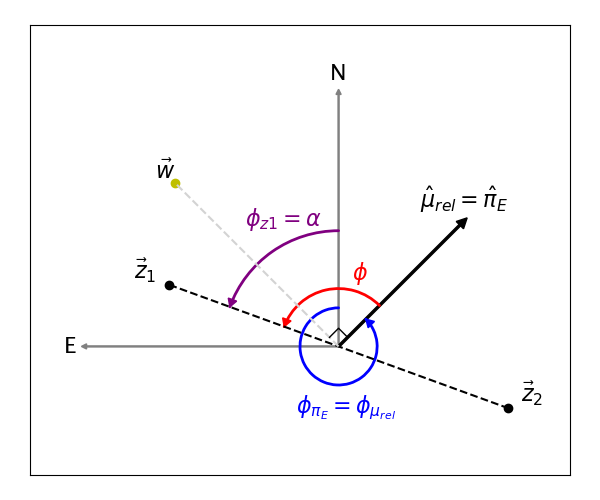
\includegraphics[width=0.45\textwidth]{figures/geometry_schematic_binary_lens.png}
    \caption{
    Binary lens geometry projected onto the sky in the complex form. 
    The binary lens is at $\vect{z}_1$ and $\vect{z}_2$. The source star 
    is at $\vect{w}$ and the direction of the relative proper motion is shown as $\murelhat$.The angle $\alpha$ is defined as the angle between North and the binary axis. $\alpha$ increments eastwards of North. $\phi_{\pi_E}$ is the angle East of North of $\hat{\mu}_{rel}$ and also $\hat{\pi}_E$. 
    \label{fig:geometry_binary}
    }
\end{figure}

The complex conjugate of Equation ~\ref{eqn:lenseqn} is:
\begin{equation}
    \bar{w} = \bar{z} - m_1 \frac{1}{z - z_1} - m_2 \frac{1}{z - z_2}.
    \label{eqn:binary_zbar}
\end{equation}
The Jacobian, which describes the transformation from source ($w, \bar{w}$) to lens ($z, \bar{z}$) plane is given by
\begin{equation}
    J = 
    \begin{bmatrix}
    \partial w / \partial z & \partial w / \partial \bar{z} \\
    \partial \bar{w} / \partial z & \partial \bar{w} / \partial \bar{z} \\
    \end{bmatrix}.
\end{equation}
Differentiating Eqns. \ref{eqn:lenseqn} and \ref{eqn:binary_zbar} gives
\begin{align}
    \frac{\partial w}{\partial z} &= \frac{\partial \bar{w}}{\partial \bar{z}} = 1 \\
    \frac{\partial \bar{w}}{\partial z} &= m_1 \frac{1}{(z - z_1)^2} + m_2 \frac{1}{(z - z_2)^2}\\
    \frac{\partial w}{\partial \bar{z}} &= m_1 \frac{1}{(\bar{z} - \bar{z}_1)^2} + m_2 \frac{1}{(\bar{z} - \bar{z}_2)^2} = \overline{\frac{\partial \bar{w}}{\partial z}}
\end{align}
which means the determinant of the Jacobian is
\begin{align}
    |J| &= \frac{\partial w}{\partial z} \frac{\partial \bar{w}}{\partial \bar{z}} - \frac{\partial w}{\partial \bar{z}} \frac{\partial \bar{w}}{\partial z} \\
    &= 1 - \left| \frac{\partial \bar{w}}{\partial z} \right|^2.
\end{align}

We can then find the amplification of the source by the lens as:
\begin{equation}
    A = \frac{1}{|J|}.
\end{equation}

There are places in which $|J| \rightarrow 0$. This corresponds to infinite amplification (if the source were a point). The curves in the lens plane where this is true are ``critical curves" and the corresponding curves in the source plane are called ``caustics." In the maps of magnification below (see \S\ref{sec:results_magmap}), we show the source plane in which we can see caustics. We also show the caustics in Figures~\ref{fig:magmaps_varyq} and \ref{fig:magmaps_varysep}. When the source passes over a caustic, this is known as a ``caustic crossing" and changes the number of lensed images of that source from 3 (when the source is outside of the caustic) to 5 (when it is inside the caustic).

To plot the critical curves and caustics, we first solve the equation $0 = |J| = 1 - \left| \frac{\partial \bar{w}}{\partial z} \right|^2$ in the lens plane by noting that the solutions correspond exactly to complex numbers $z$ satisfying 
\begin{align}
\frac{\partial \bar{w}}{\partial z} = m_1 \frac{1}{(z - z_1)^2} + m_2 \frac{1}{(z - z_2)^2} = e^{i\theta}
\end{align}
for some $\theta \in [0,2\pi)$. Clearing the denominators produces a quartic polynomial in $z$ with coefficients depending on $z_1,z_2,m_1,m_2,$ and $\theta$. Points along the critical curve are calculated by solving the four roots of this polynomial for a range of $\theta$ values, and the corresponding caustic curve can then be plotted by using the lens equation to map points from the lens plane to the source plane. Examples of critical and caustic curves are shown in Figure~\ref{fig:magmaps_varyq} and Figure~\ref{fig:magmaps_varysep} for a range of different binary lens separations and mass ratios.

In the microlensing models added to BAGLE, we parameterize our models such that we know where the source is in the source plane ($w$), where the binary lenses are in the lens plane ($z_1$ and $z_2$), the masses of the two lenses, and the distance to all objects. Therefore, we are solving for the observed position of the source in the lens plane ($z$).

In order to avoid working with an equation with a mix of complex numbers and their conjugates, it is standard to plug Eqn.~\ref{eqn:binary_zbar} into Eqn.~\ref{eqn:lenseqn} and simplify \citep[see][]{Witt1990, WittShude1995}. This yields a fifth-order polynomial known as the ``lens polynomial." This typically yields the same solutions as the ``lens equations," but sometimes has additional solutions which must be verified (see \S~\ref {sec:binlenses_eqn2}).

The number of real solutions given by solving the lens polynomial depends on the position of the source. When the source is inside a caustic, there are five solutions. When the source is outside the caustic, there are three solutions. 


\subsection{Solving the Binary Lens Equation in BAGLE}
\label{sec:binlenses_eqn2}

Given a microlensing model and a set of microlensing parameters, we need to determine the position and magnification of each image.

In BAGLE, we use parameters such that we know the location of the source ($w$, source plane), the lens positions ($z_i$, lens plane) and masses, as well as the distances to all objects.
In other words, what we need to know $z$ which is where the light ray hits the lens plane.

When the source is inside a caustic, there are five images; when the source is outside the caustic, there are three images. Thus, when we solve the lens polynomialfor a source outside of a caustic, two of our solutions will be invalid.

We need the amplifications and centroids of the images. The high-level step-by-step algorithm is:

\begin{enumerate}
    \item Solve the lens polynomial using \texttt{np.roots()}, obtain 5 solutions. In cases where the source is far away from the caustic, figure out which 3 of those five solutions are valid by substituting them into the lens equation and seeing what works. These three solutions $\vec{r}_j$ are the locations of the images in the lens plane.
    \item Evaluate the inverse Jacobian ($J$) at these three points to get the magnifications of the images $A_j = \frac{\partial \vect{x}}{ \partial \vec{r}} |_{\vec{r}_j}$. 
    \item Then we can calculate the magnification and position of the centroid at any given time: 
    \begin{align}
        A &= \sum_j A_j  = \frac{1}{|J|}\\
        \vec{r} &= \frac{\sum_j A_j \vec{r}_j}{\sum_j A_j}
    \end{align}
\end{enumerate}


\section{Binary Sources and Binary Lenses (BSBL) \label{sec:bineverything}}
 
\begin{figure*}
    \centering
    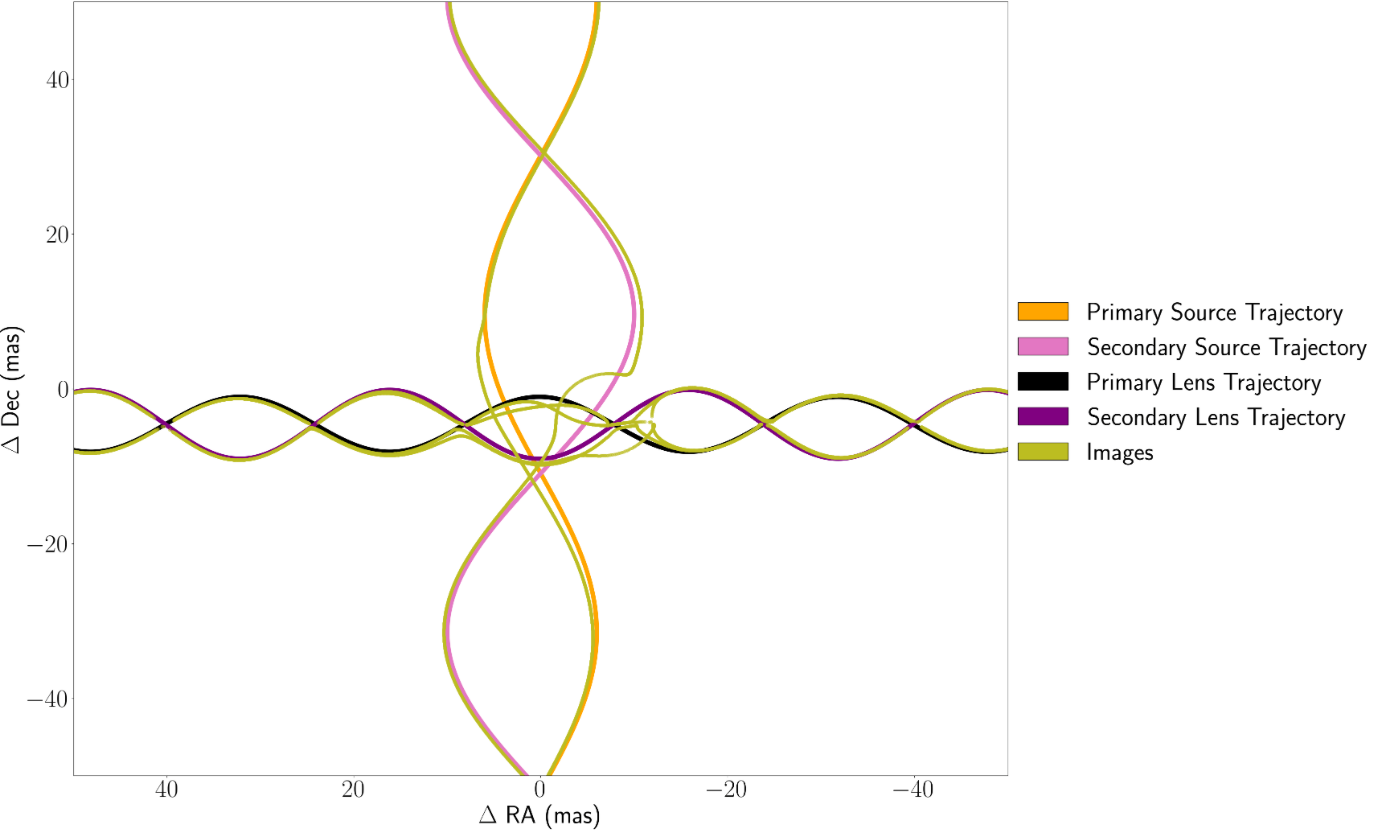
\includegraphics[width= \textwidth] {figures/bsbl_keplerian.png}
    \caption{Source and lens trajectories for a simulated binary source, binary lens microlensing event with  involving circular orbits. The orange line is the primary source, the pink line is the secondary source, the black line is the primary lens, the purple line is the secondary lens, and the yellow lines are the image positions. The simulation was run with a $t_E = 231.15$ days with the following orbital parameters for the lens: $\w = 30 \degree$, $\bigomega = 10 \degree$, $\inclination = 90 \degree$, $e=0$, $\period = 1948.04 $ days, and the following orbital parmaeters for the source $\w = 30 \degree$, $\bigomega = 10 \degree$, $\inclination = 90 \degree$, $e=0.6$, $\period = 6000 $ days. The lenses have a mass of $m_{L,p}=$ 10 $M_\odot$ and $m_{L,s}=$ 8 $M_\odot$.}
    \label{fig:bsbl_keplerian}
\end{figure*}


 BAGLE can also simulate events with both binary sources and binary lenses. The orbital and lensing equations necessary to simulate a binary source and binary lens event in BAGLE are individually handled. This means that the equations necessary to simulate binary sources are from \S\ref{sec:binsource}, and the equations necessary to simulate binary lenses are from Sec. \S\ref{sec:binlenses}.

For BSBL events with static, linear or accelerated approximations, $\tnot$ is defined as the time of closest approach between the geometric midpoint of the lens and the primary source. However, for Keplerian orbital motion (circular and elliptical), $\tnot$ is defined as the time of closest approach between the center of masses of the binary lens and the binary source. 

We present our astrometric simulations in Figure~\ref{fig:bsbl_keplerian}. \texttt{BSBL\_PhotAstrom\_noPar\_CircOrbs\_Param2} is the binary source and binary lens model from BAGLE that is used to simulate a circular orbital solution for such a microlensing event. The BSBL model assumes that both - the source and the lens - display orbital motion. 

\section{Validation of Models}
\label{sec:validation}

\begin{figure}
    \centering
    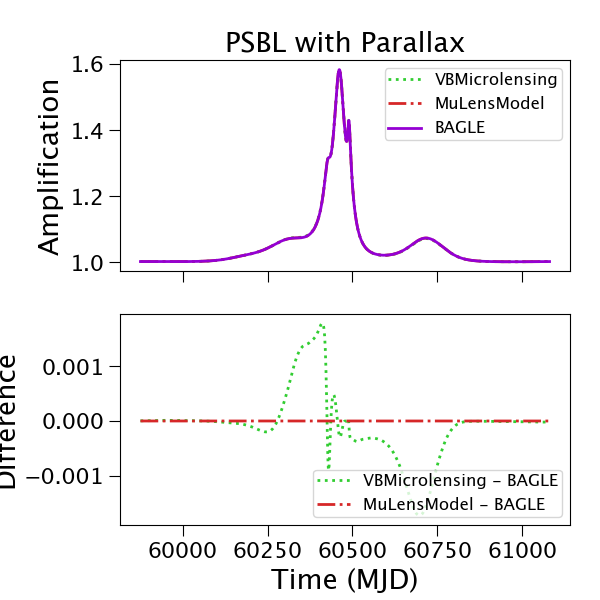
\includegraphics[width= .48 \textwidth]{figures/parallax_comparison.png}
    \caption{Comparison of a simulated PSBL event with parallax between VBMicrolensing, MuLensModel and BAGLE. The microlensing parameters in the SSB lens-frame are: $\tnot = 60478.49$, $\uo=1 \,\thetaE$, $\tE = 100.4$ days, $q = 0.3$, $\piE = [0.5, 0.5] \thetaE$. The amplification  ({\em top}) and residuals with respect to the BAGLE model ({\em bottom}) are shown over time.}
    \label{fig:parallax_comparison}
\end{figure}


In this section, we compare BAGLE with other contemporary microlensing models (VBMicrolensing and MuLensModel) against simulated point-source binary-lens events with parallax, but without orbital motion. A comparison with the inclusion of orbital motion is reserved for future. 

We begin by creating a BAGLE model using the parameterization \texttt{PSBL\_Phot\_Par\_Param1}. \texttt{PSBL\_Phot\_Par\_Param1} inputs quantities with reference to the geometric midpoint of the lens system, and calculates Earth's position relative to the Solar System Barycenter over time. Event parameters in BAGLE are: $\tnot = 60478.49$, $\uo=1 \,\thetaE$, $\tE = 100.4$ days, $q = 0.3$, $\piE = [0.5\thetaE, 0.5\thetaE]$. The relative angle between the binary system and the $\murel$ directional vector in degrees is given by $\phi=125 \degree$. The two lenses have a separation of $0.8 \,\thetaE$. 

In contrast to BAGLE, other packages prefer a geo-projected frame of reference (an argument explored in \citet{Lu:2025}). The resulting geo-projected parameters are  $\tnotgeotr = 60458.64$, $\uogeotr= 0.92 \,\thetaE$, $\tE = 49.52$ days, $q = 0.3$, $\piE = [-0.67 \thetaE, -0.24 \thetaE] $. After converting to the geo-projected frame of reference, an additional transformation must be applied to $\uvecgeotr$ and $\tnotgeotr$ in order to switch from the geometric midpoint of the lens to the center of mass. The final $\tnotgeotr$ and $\uvecgeotr$ input to VBMicrolensing and MuLensModel are $60461.78$ and $0.67$, respectively. 

The comparison between VBM, MulensModel, and BAGLE is shown in Figure \ref{fig:parallax_comparison}. Differences of 10$^{-4}$ are apparent between BAGLE and VBM. These differences are due to the different microlensing frame of reference used for input parameters.

%We present our comparison between VBMicrolensing, MuLens and BAGLE in Figure~\ref{fig:parallax_comparison}. We observe differences at an order of magnitude of $-4$ with VBMicrolensing and $-12$ with MuLensModel. We attribute these differences to the different microlensing frame of reference used for input parameters. 

%\textcolor{red}{PLOTS}

%\section{Validation of Models}
%\textcolor{red}{ONLY WRITTEN THE EQUATIONS TILL NOW}
%\subsection{Cases without Orbital Motion}
%\subsubsection{No Parallax}
%$$\phi_{Gould} = \alpha_{Gould} =  - \phi_{BAGLE}$$

%$$q' = \frac{1-q}{2*(1+q)}$$

%$$u0_{MuLens} = u0_{pyLIMA} = u0 + q' * sep * sin(\phi_{Gould})$$

%$$t0_{MuLens} = t0_{pyLIMA} = t0_{BAGLE} + q' * sep_{BAGLE} * tE_{BAGLE} * cos(\phi_{Gould}) + 2400000.5$$

%$$t0_{VBM} = t0_{pyLIMA} - 2400000.5$$

%$$q_{MuLens} = 1/q_{BAGLE}$$

%$$\rho_{VBMicrolensing} = 10^{-8}$$
%\subsubsection{Parallax}
%Same but geo


%\begin{figure*}
 %   \centering
  %  \includegraphics[width=0.7\textwidth] {figures/nopar.png}
   % \caption{}
    %\label{fig:nopar}
%\end{figure*}

%\begin{figure*}
 %   \centering
  %  \includegraphics[width=0.7\textwidth] {figures/par.png}
   % \caption{}
    %\label{fig:par}
%\end{figure*}






%\subsection{Cases with Orbital Motion }
%\textcolor{red}{This is very broken right now}


%\textcolor{red}{TODO. Rough conversions written here; have to recheck for OM}
%Only for point source binary lenses. 
%Binary source conversions look straightforward. 
%Can we just link to the tutorial instead of having all the conversions here?

%No orbital motion:

%$\alpha = \phi + \piE$
%$\phi_{rad, pylima}=-\phi$
%For no orbital motions, we operate in $\uo$, $\tnot$ at geometric center of lens. Switch to $\tcomnot$ and $\uocom$. LINK TO APPENDIX CONVERSIONS

%Above works for no parallax

%For parallax switch to geocentric coordinates. Switch to com using geocentric t0s and u0s. (WE CAN WRITE ALL THIS IN APPENDIX)

%include figures

%Should we include OM since not fully complete? We can say OMs confusing rn, not fully complete. VBM only one with full orbital motion. I think this is a better idea, because doing conversions for orbial parameters between all the different models can be a whole different paper. We compare BAGLE with MuLens and PyLima for linear approximations, and VBM for full Keplerian solutions. 

%\section{Validation of Models for No Orbital Motion}



\begin{deluxetable}{p{1.5in}c}
\tablecaption{Parameters used to generate the mock dataset using \texttt{BSPL\_PhotAstrom\_noPar\_EllOrbs\_Param1}. \label{tab:fake_fit}}
\tablehead{
\colhead{\textbf{Parameter}} & \colhead{\textbf{Value}}
}
\startdata
\texttt{$m_L$} & $20\,M_\odot$ \\
\texttt{$\tcomnot$} & 57000 \\
\texttt{$\uocom$} & 0.75 \\
\texttt{$dL$} & $1000 \, pc$ \\
\texttt{$dL\_dS$} & 0.1 \\
\texttt{$\Xsvec$} & [0, 0] \\
\texttt{$\mulsvec$} & [0, 0] $\frac{mas}{yr}$ \\
\texttt{$\mussysvec$} & [8, 3] $\frac{mas}{yr}$ \\
\texttt{$\omega$} & $30 \degree$ \\
\texttt{$\Omega$} & $10^\degree$ \\
\texttt{$\inclination$} & $0^\degree$ \\
\texttt{$\eccentricity$} & 0.5 \\
\texttt{$\period$} & 450 days \\
\texttt{$\al$} & 2 mas \\
\texttt{$\ala$} & 2.5 mas \\
\texttt{$b_{sff}$} & 1 \\
\texttt{$mag_{S,pri}$} & 18 \\
\texttt{$mag_{S,sec}$} & 20 \\
\enddata
\end{deluxetable}


\section{Results}
\label{sec:results}

The inclusion of binary models in the \bagle~ package enables us to explore many different aspects of binary microlensing events. In this section, we explore some of the most notable impact of including binary models in the \bagle~package.

allows us to explore many aspects of microlensing events. 

In this section, we investigate
\begin{itemize}
    \setlength\itemsep{0em}
    \item \S\ref{sec:results_magmap} - Magnification Maps. 
    \item \S\ref{sec:results_asm} - Centroid Shift Maps. 
    \item \S\ref{sec:results_q} - Dependency of mass ratio on caustic structures. 
    \item \S\ref{sec:results_om} - Dependency of orbital motion on fitting. 
\end{itemize}

\subsection{Results: Magnification Maps}

\begin{figure}
    \centering
    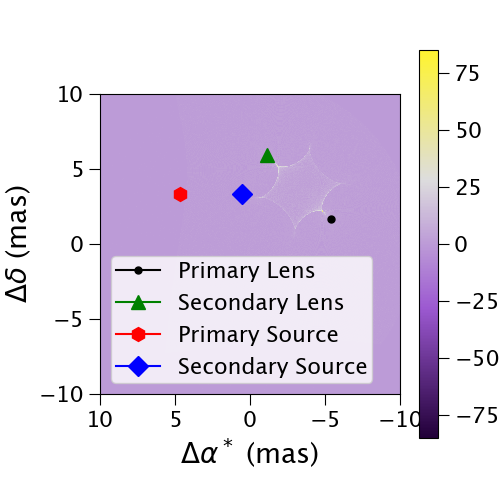
\includegraphics[width= 0.48 \textwidth]{figures/magmap.png}
    \caption{Magnification map for a BSBL microlensing event with both the source and lens at $\tcomnot$. The contour of the magnification map is indicative of the caustic. }
    \label{fig:magmaps}
\end{figure}


\label{sec:results_magmap}

By solving the lens equation, the magnification of the source at any (projected) position relative to the position of the lens can be calculated. The magnification map is a visualization reflecting the calculated magnification at a given point. Magnification maps are generated using the inverse ray shooting method \citep{Bennett_2010}. The inverse ray shooting method is a simple way to invert the lens equation by shooting
rays backwards from the observer to the lens.

\begin{itemize}
    \item Create a sample grid of image positions in the lens frame of reference. 
    \item Calculate information about the lens, i.e., the lens positions at the time of closest approach (between the source and the lens system’s center of mass) and the lens mass ratio.
    \item Use the lens mass ratio, lens positions, the image grid, and the source position to get the lensed source positions. 
    \item By mapping the image grid to the source plane and then binning the resulting source positions, the magnification map indicates how many rays fall into each pixel in the source plane grid. More rays imply a higher magnification. The magnification map we present in Figure ~\ref{fig:magmaps} is purely statistical. 
\end{itemize}

The magnification map for a BSBL event at $t_p$ is presented in Figure ~\ref{fig:magmaps}. The large boundaries of amplification in the magnification map are caustics. Caustics are characteristic features of the photometric curves of binary lenses. Since the sources have a finite size, their amplification does not become infinitely high. However, it still presents itself in the form of sharp peaks in our lightcurves. 

\subsection{Centroid Shift Maps}
\label{sec:results_asm}

\begin{figure}
    \centering
    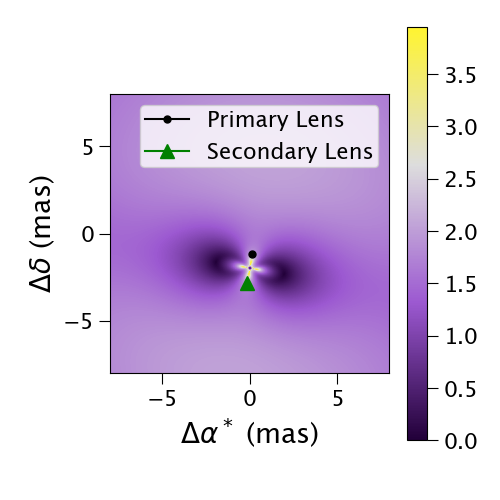
\includegraphics[width= 0.48 \textwidth]{figures/csmap.png}
    \caption{A color map for the centroid shift during a PSBL microlensing event with the lenses at the time of closest approach. The color scale indicates the absolute centroid shift in the image plane.}
    \label{fig:csmap}
\end{figure}

Like the magnification map, a forward ray shooting method can be used to shoot from the source plane to the image plane, creating a color map of centroid shift. This forward ray shooting method works in the following way:


\begin{itemize}
    \item Create a sample grid of source positions. 
    \item Solve the lens equation to get all possible image positions using the sample grid of source positions. Find the flux-weighted centroids of these possible image positions.
    \item Bin the flux-weighted centroids to create a color map of how many rays fall into each pixel in the image plane grid. Normalize it by using the flux-weighted centroids on the colorbar. 
\end{itemize}

A centroid shift color map for a PSBL event at $t_p$ is presented in Figure~\ref{fig:csmap}. The color scale indicates the absolute centroid shift.



\subsection{Results: Dependency of Mass Ratio and Separation}


\begin{figure*}
    \centering
    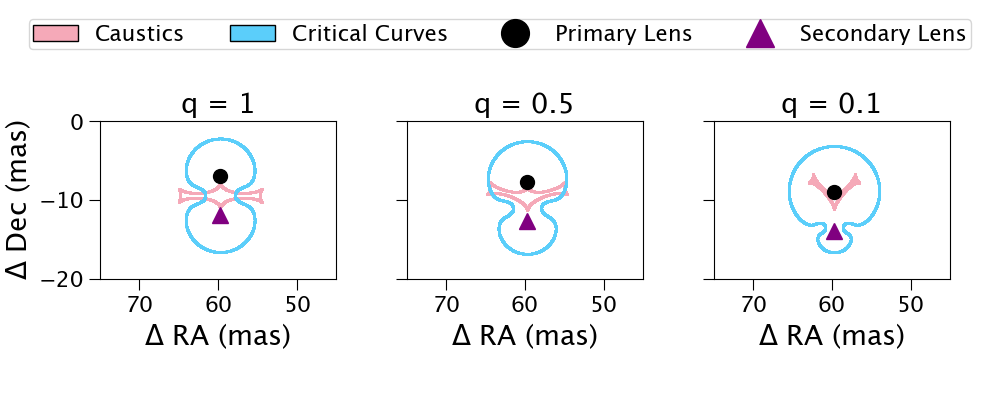
\includegraphics[width= \textwidth]{figures/magmaps_varyq.png}
    \caption{Caustics (\emph{pink}) and critical curves (\emph{blue}) for a PSBL model with the lens at a separation of 5 mas. We present panels with $q$ ranging from 0.1 to 1.}
    \label{fig:magmaps_varyq}
\end{figure*}



\begin{figure*}
    \centering
    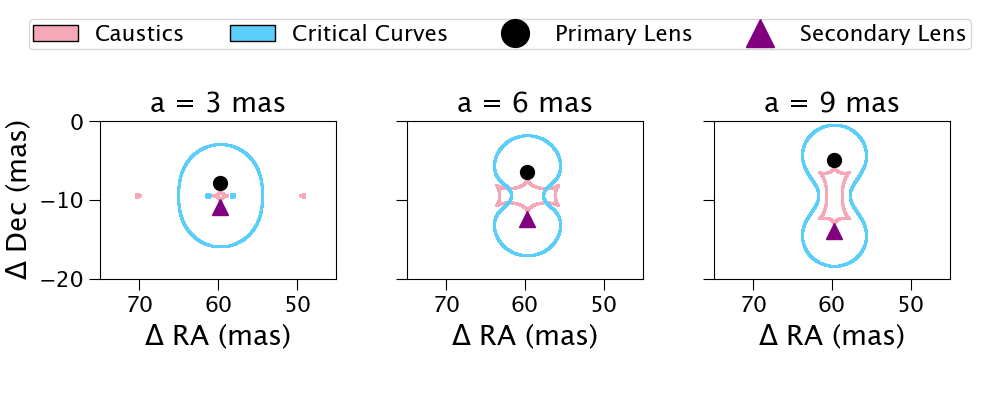
\includegraphics[width= \textwidth]{figures/magmaps_varysep.png}
    \caption{Caustics (\emph{pink}) and critical curves (\emph{blue}) for a PSBL model at $t_p$ with a fixed $q=1$. The value of $a$ (provided as an input to the PSBL models) varies between $3$ mas, $6$ mas, $9$ mas in the three panels.}
    \label{fig:magmaps_varysep}
\end{figure*}

\label{sec:results_q}
In this section, we explore the dependency of caustics on mass ratios and separation. The separation is fixed at an arbitrarily chosen value of 3 mas and the mass ratio $q=\frac{m_{L,s}}{m_{L,p}}$ for a dark, non-planetary lens, ranges from 0.1 to 1. The caustics and critical curves are presented in Figure~\ref{fig:magmaps_varyq}. We see that the caustic becomes more symmetric as $q \rightarrow 1$. The degree of asymmetry is directly dependent on $q$. 

Similarly, by fixing the mass  $q=\frac{m_{L,s}}{m_{L,p}} = 1$, BAGLE can replicate a dark, non-planetary lens at varying angular separations between the primary and secondary lens. From the caustics and critical curves presented in Figure~\ref{fig:magmaps_varysep}, we see that the caustic remains symmetric regardless of separation for a fixed $q=1$. At larger separations, the caustics also become increasingly elongated or stretched. Detailed descriptions of the geometry of caustics for the q = 1 case can be found in \cite{Schneider_1986}.  




\begin{figure*}
    \centering
    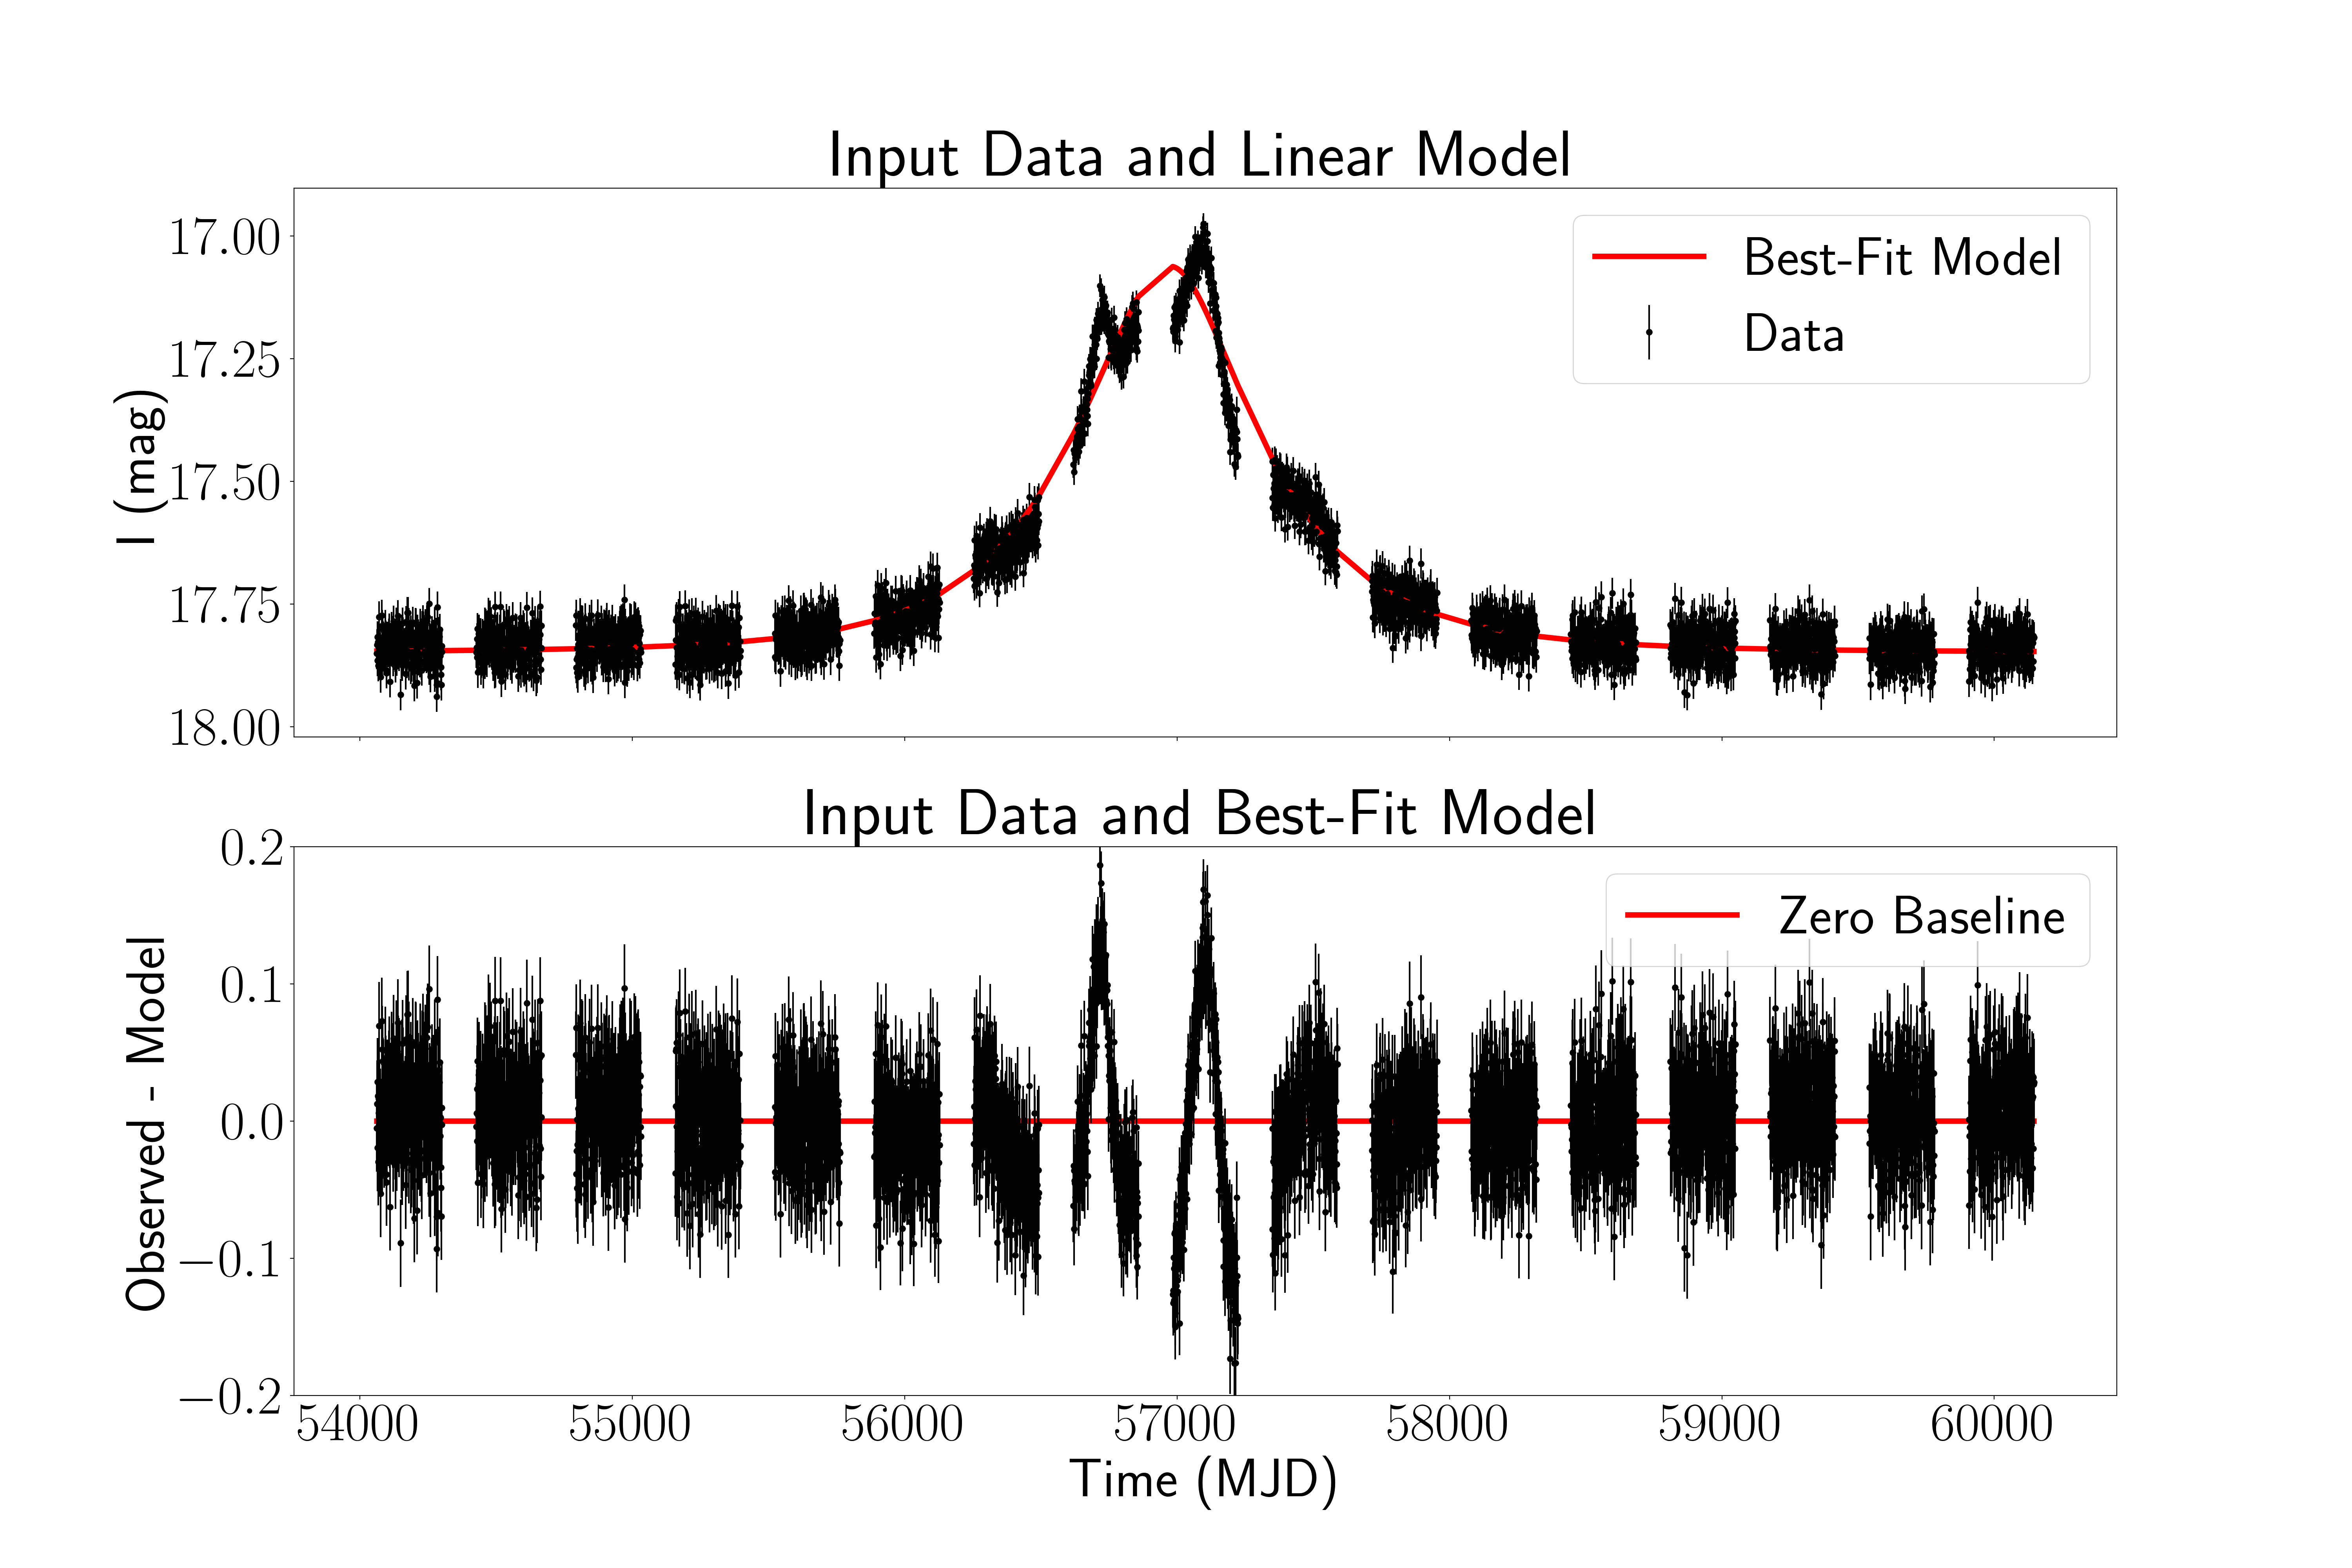
\includegraphics[width= .48 \textwidth]{figures/LinAnal.png}
    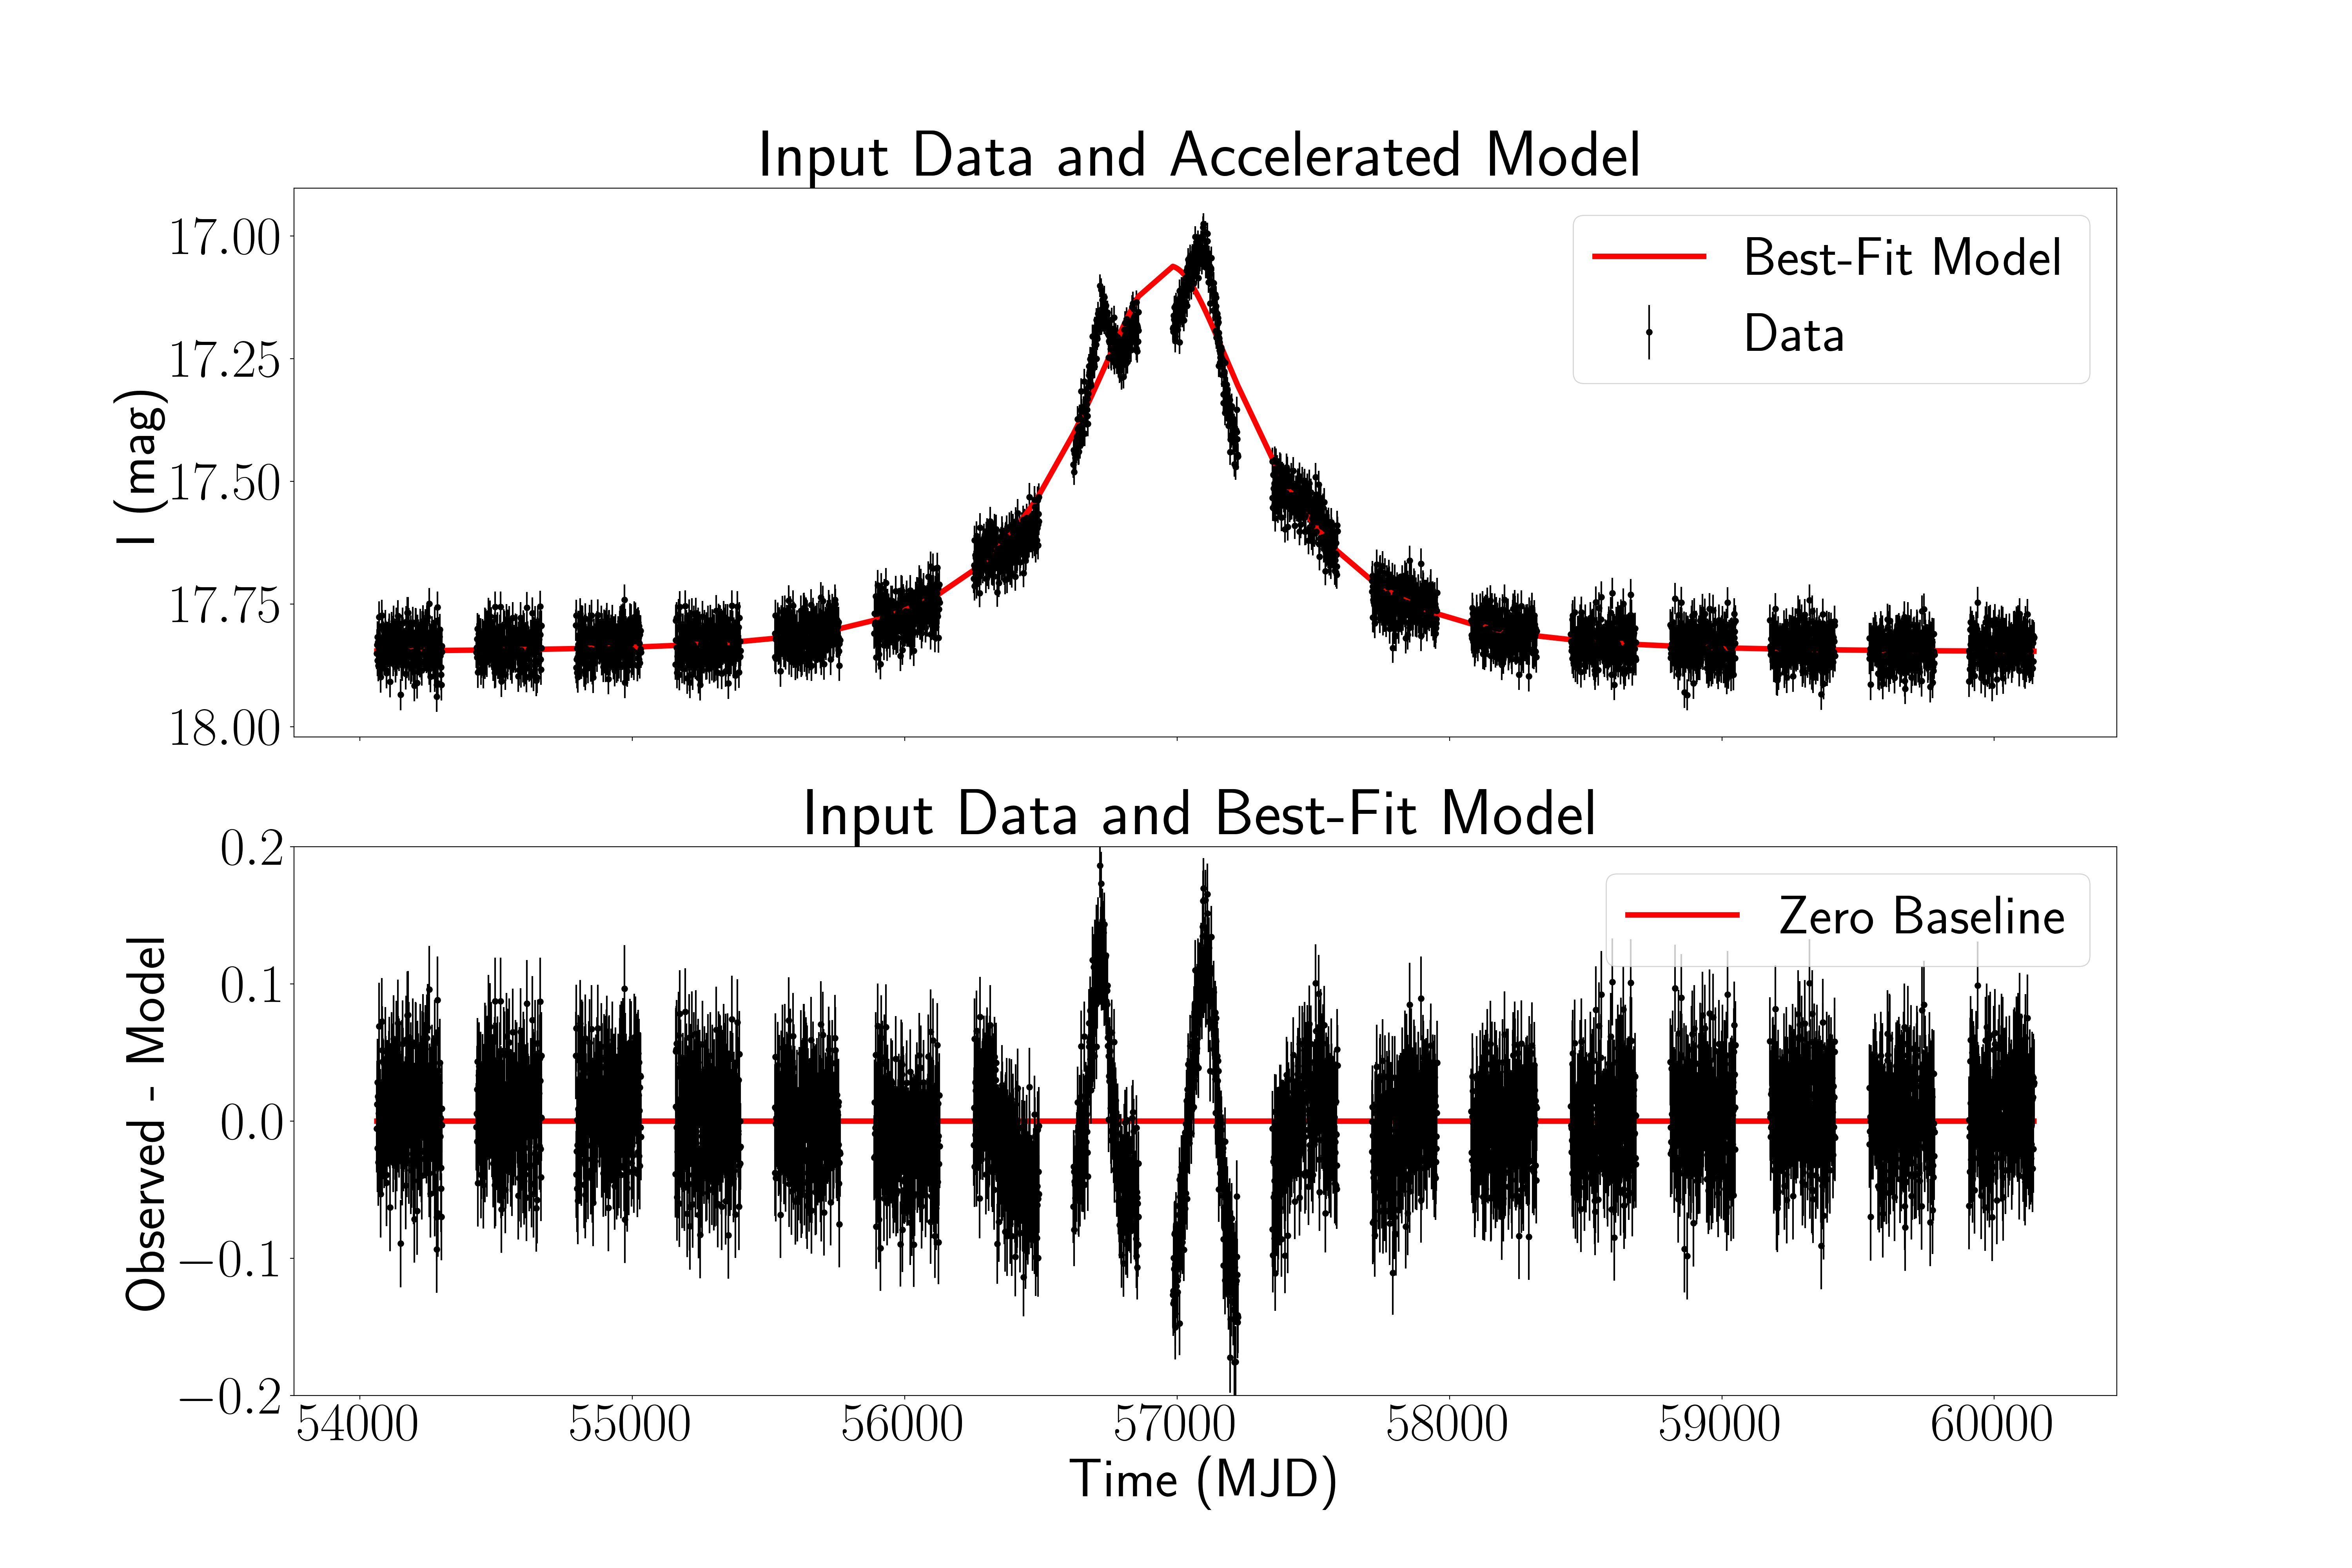
\includegraphics[width= .48 \textwidth]{figures/AccAnal.png}
    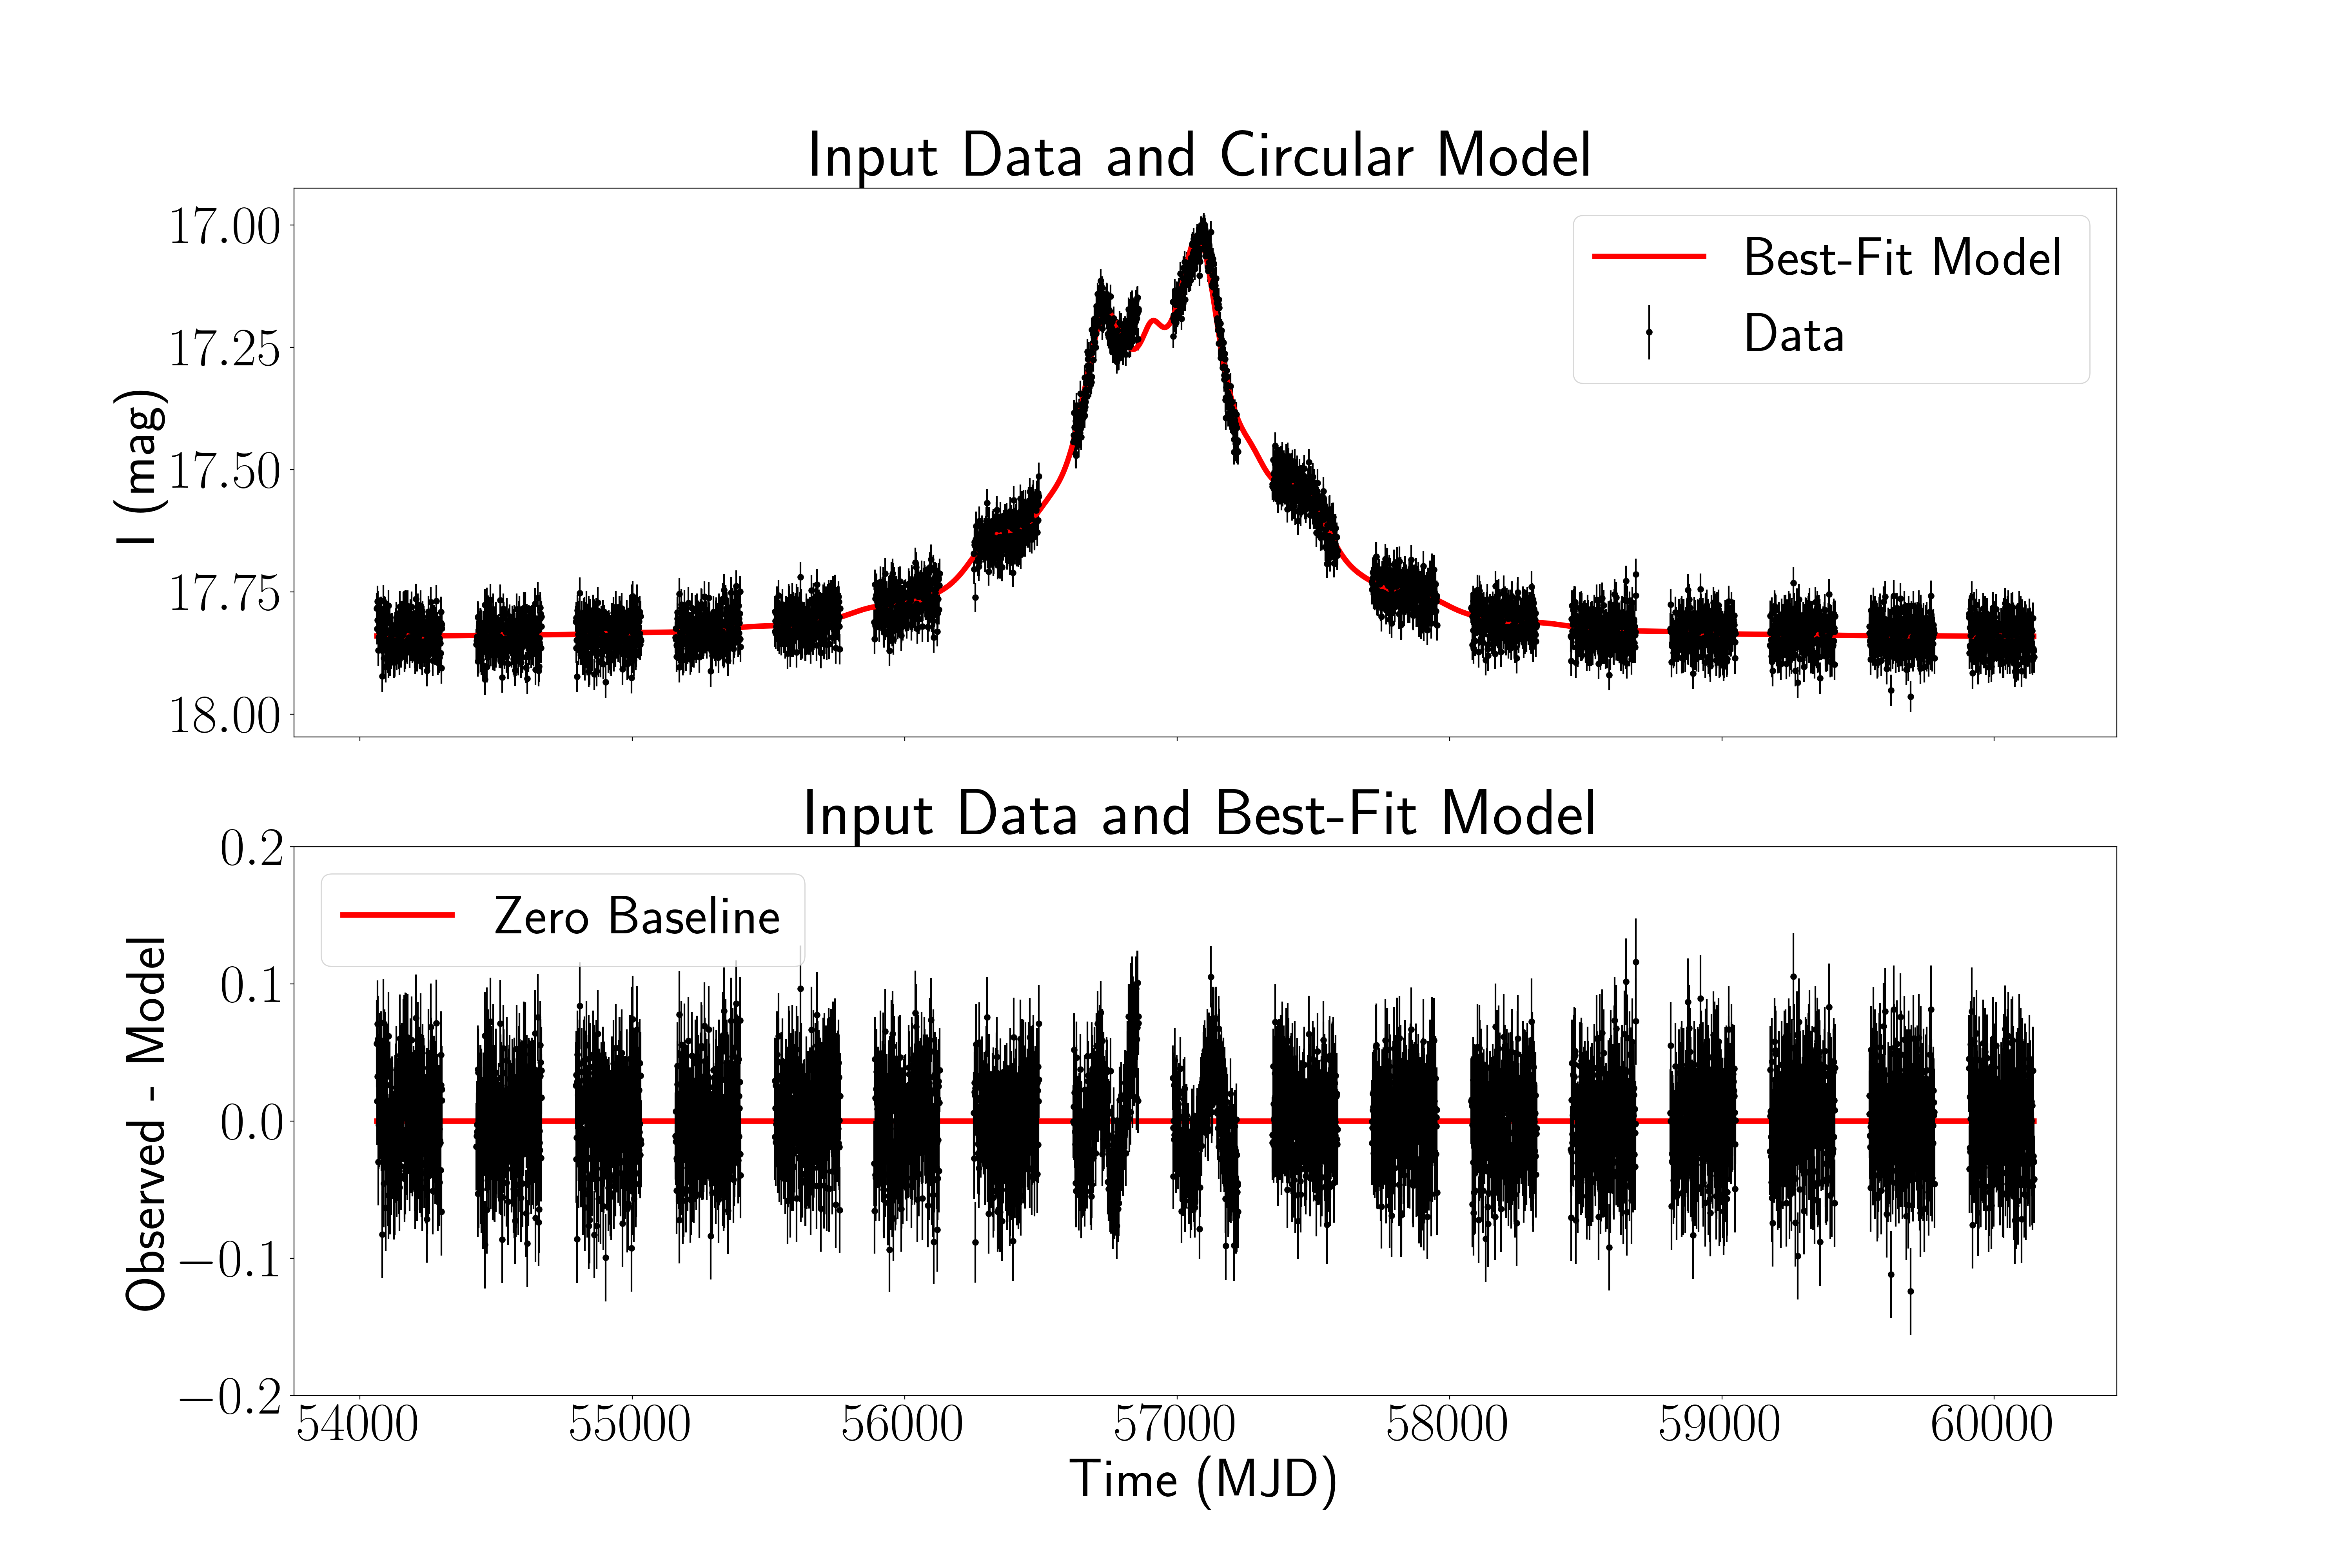
\includegraphics[width= .48\textwidth]{figures/CircAnal.png}
    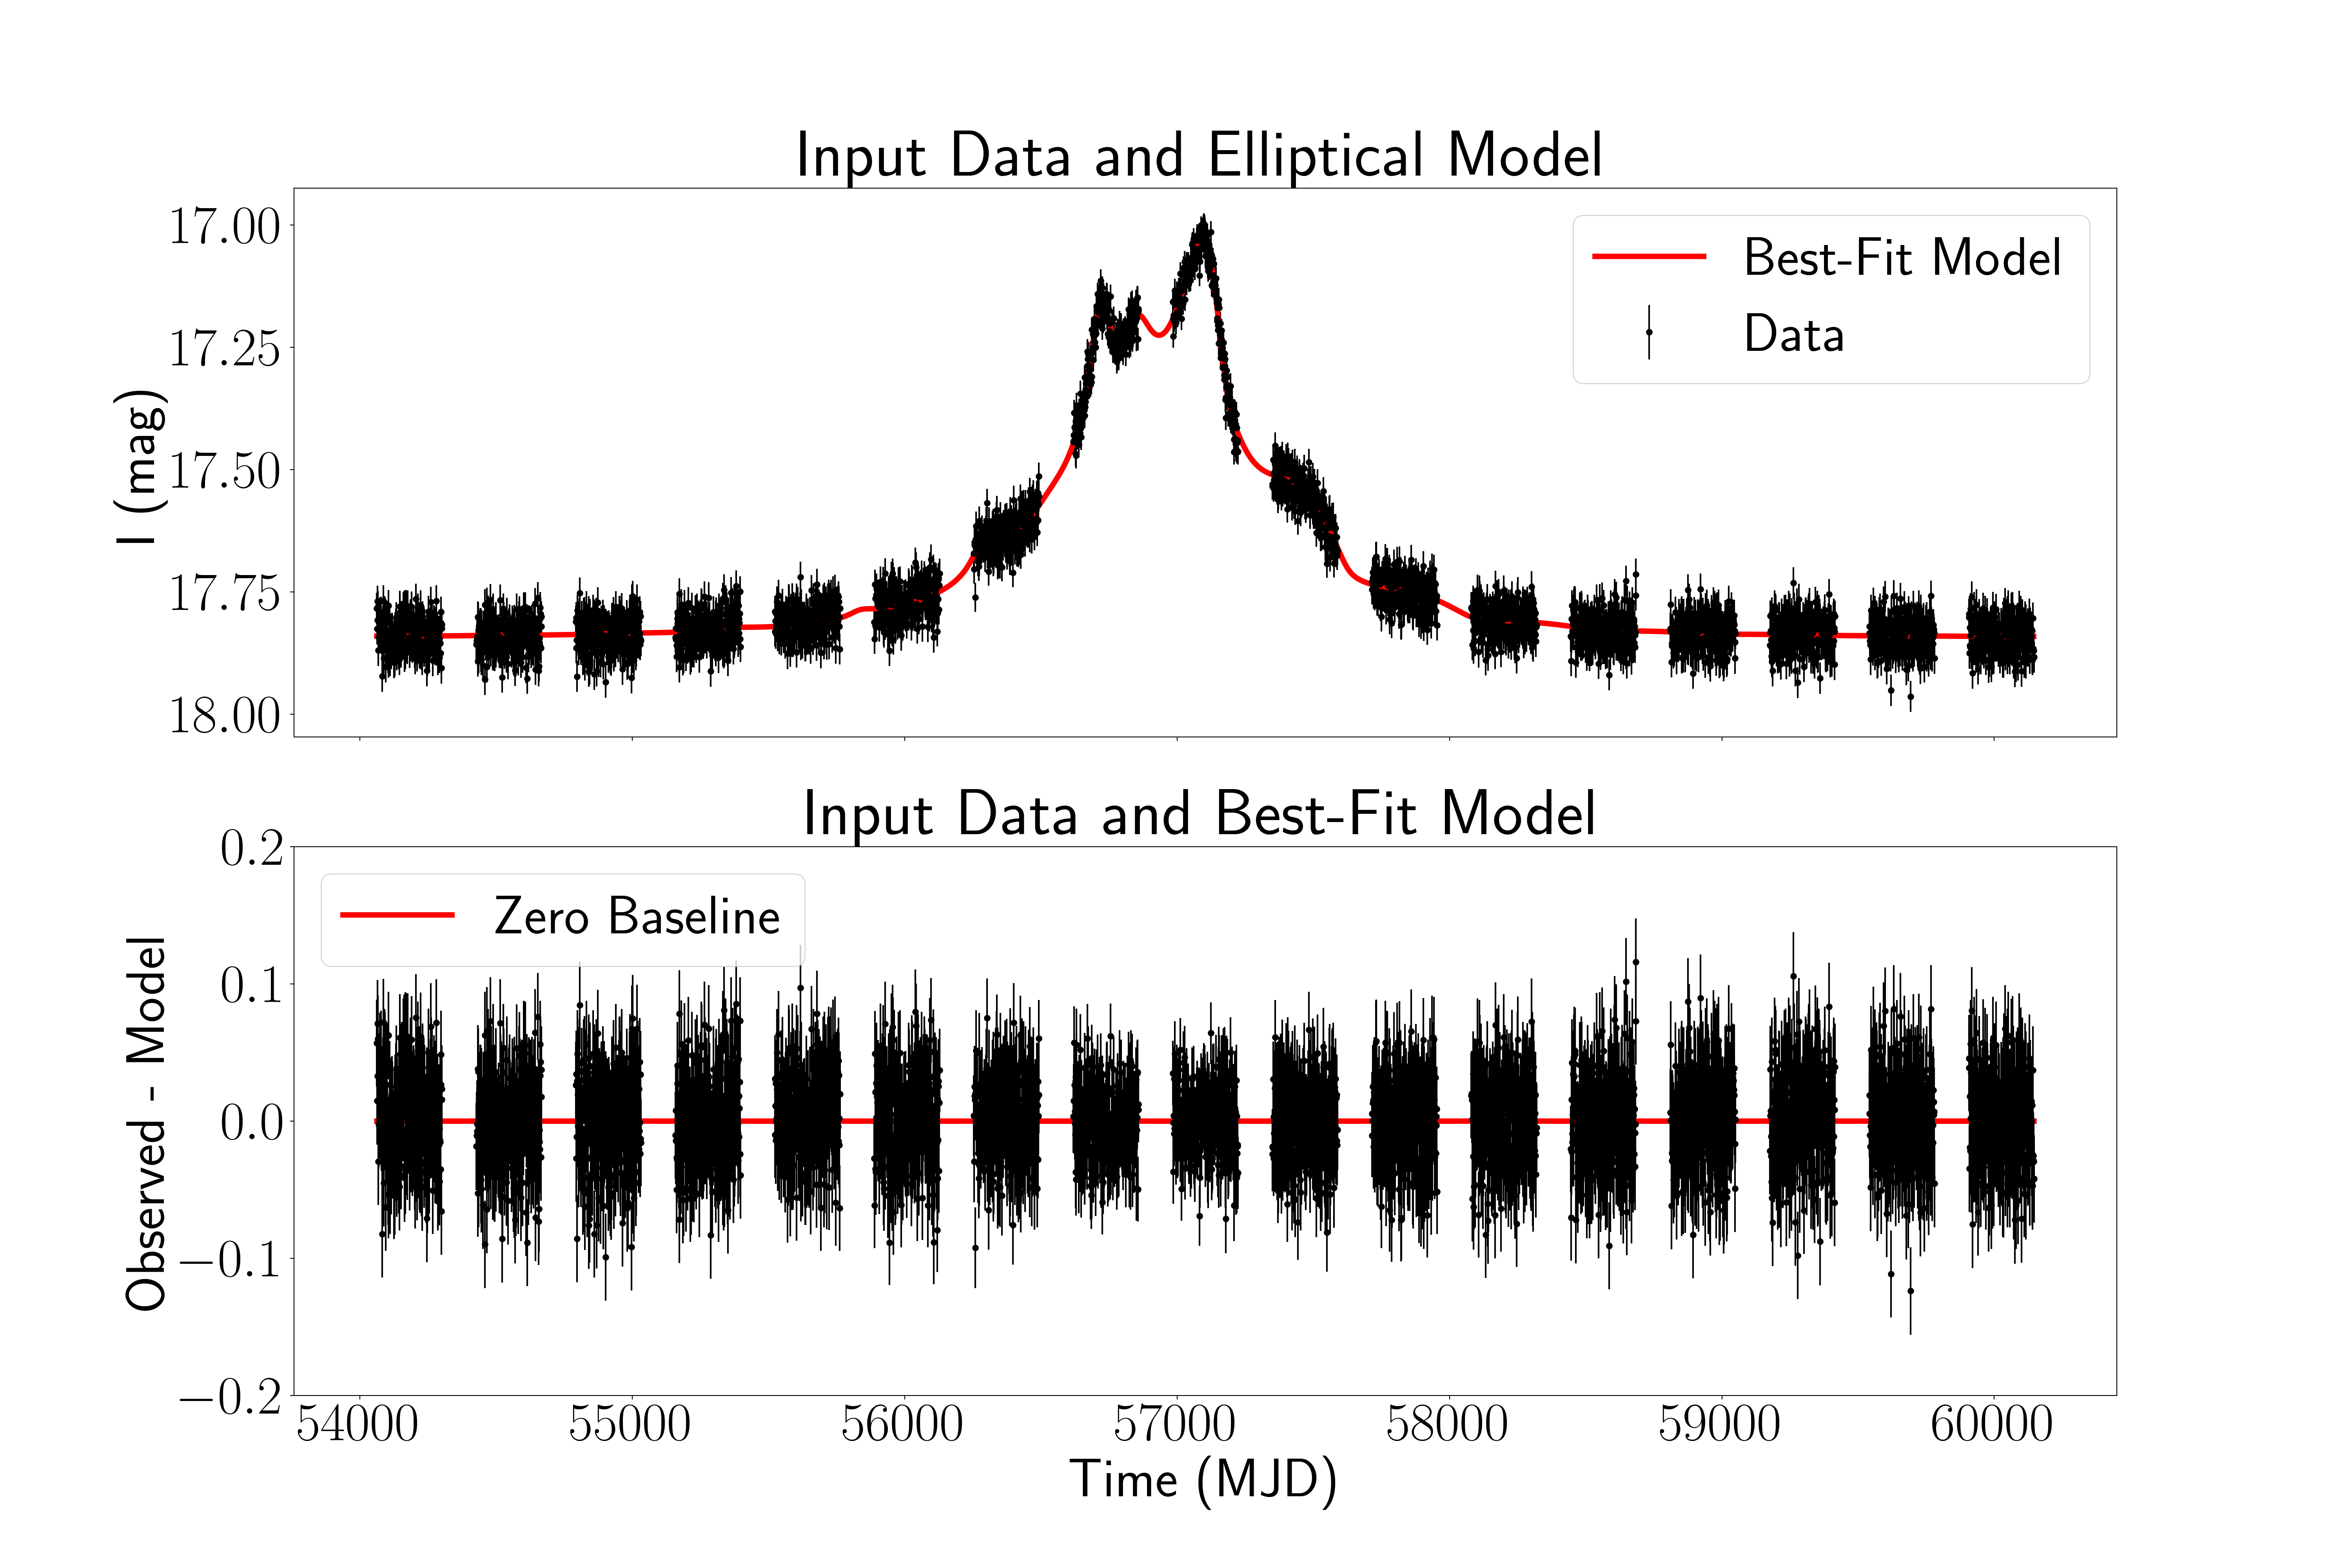
\includegraphics[width= .48\textwidth]{figures/EllAnal.png}

    \caption{Fitting output for a mock photometric dataset generated using  BSPL\_PhotAstrom\_noPar\_EllOrbs\_Param1 and the parameters displayed in Table ~\ref{tab:fake_fit}. We see correlated residuals in the linear and accelerated fits, unlike the circular and elliptical fits. 
    (\emph{Top Left}) Best-fit with linear orbital motion. (\emph{Top Right}) Best-fit with accelerated orbital motion. (\emph{Bottom Left}) Best-fit with circular orbital motion. (\emph{Bottom Right}) Best-fit with elliptical orbital motion}
    \label{fig:orbital_comparison}
\end{figure*}



\begin{figure*}
    \centering
    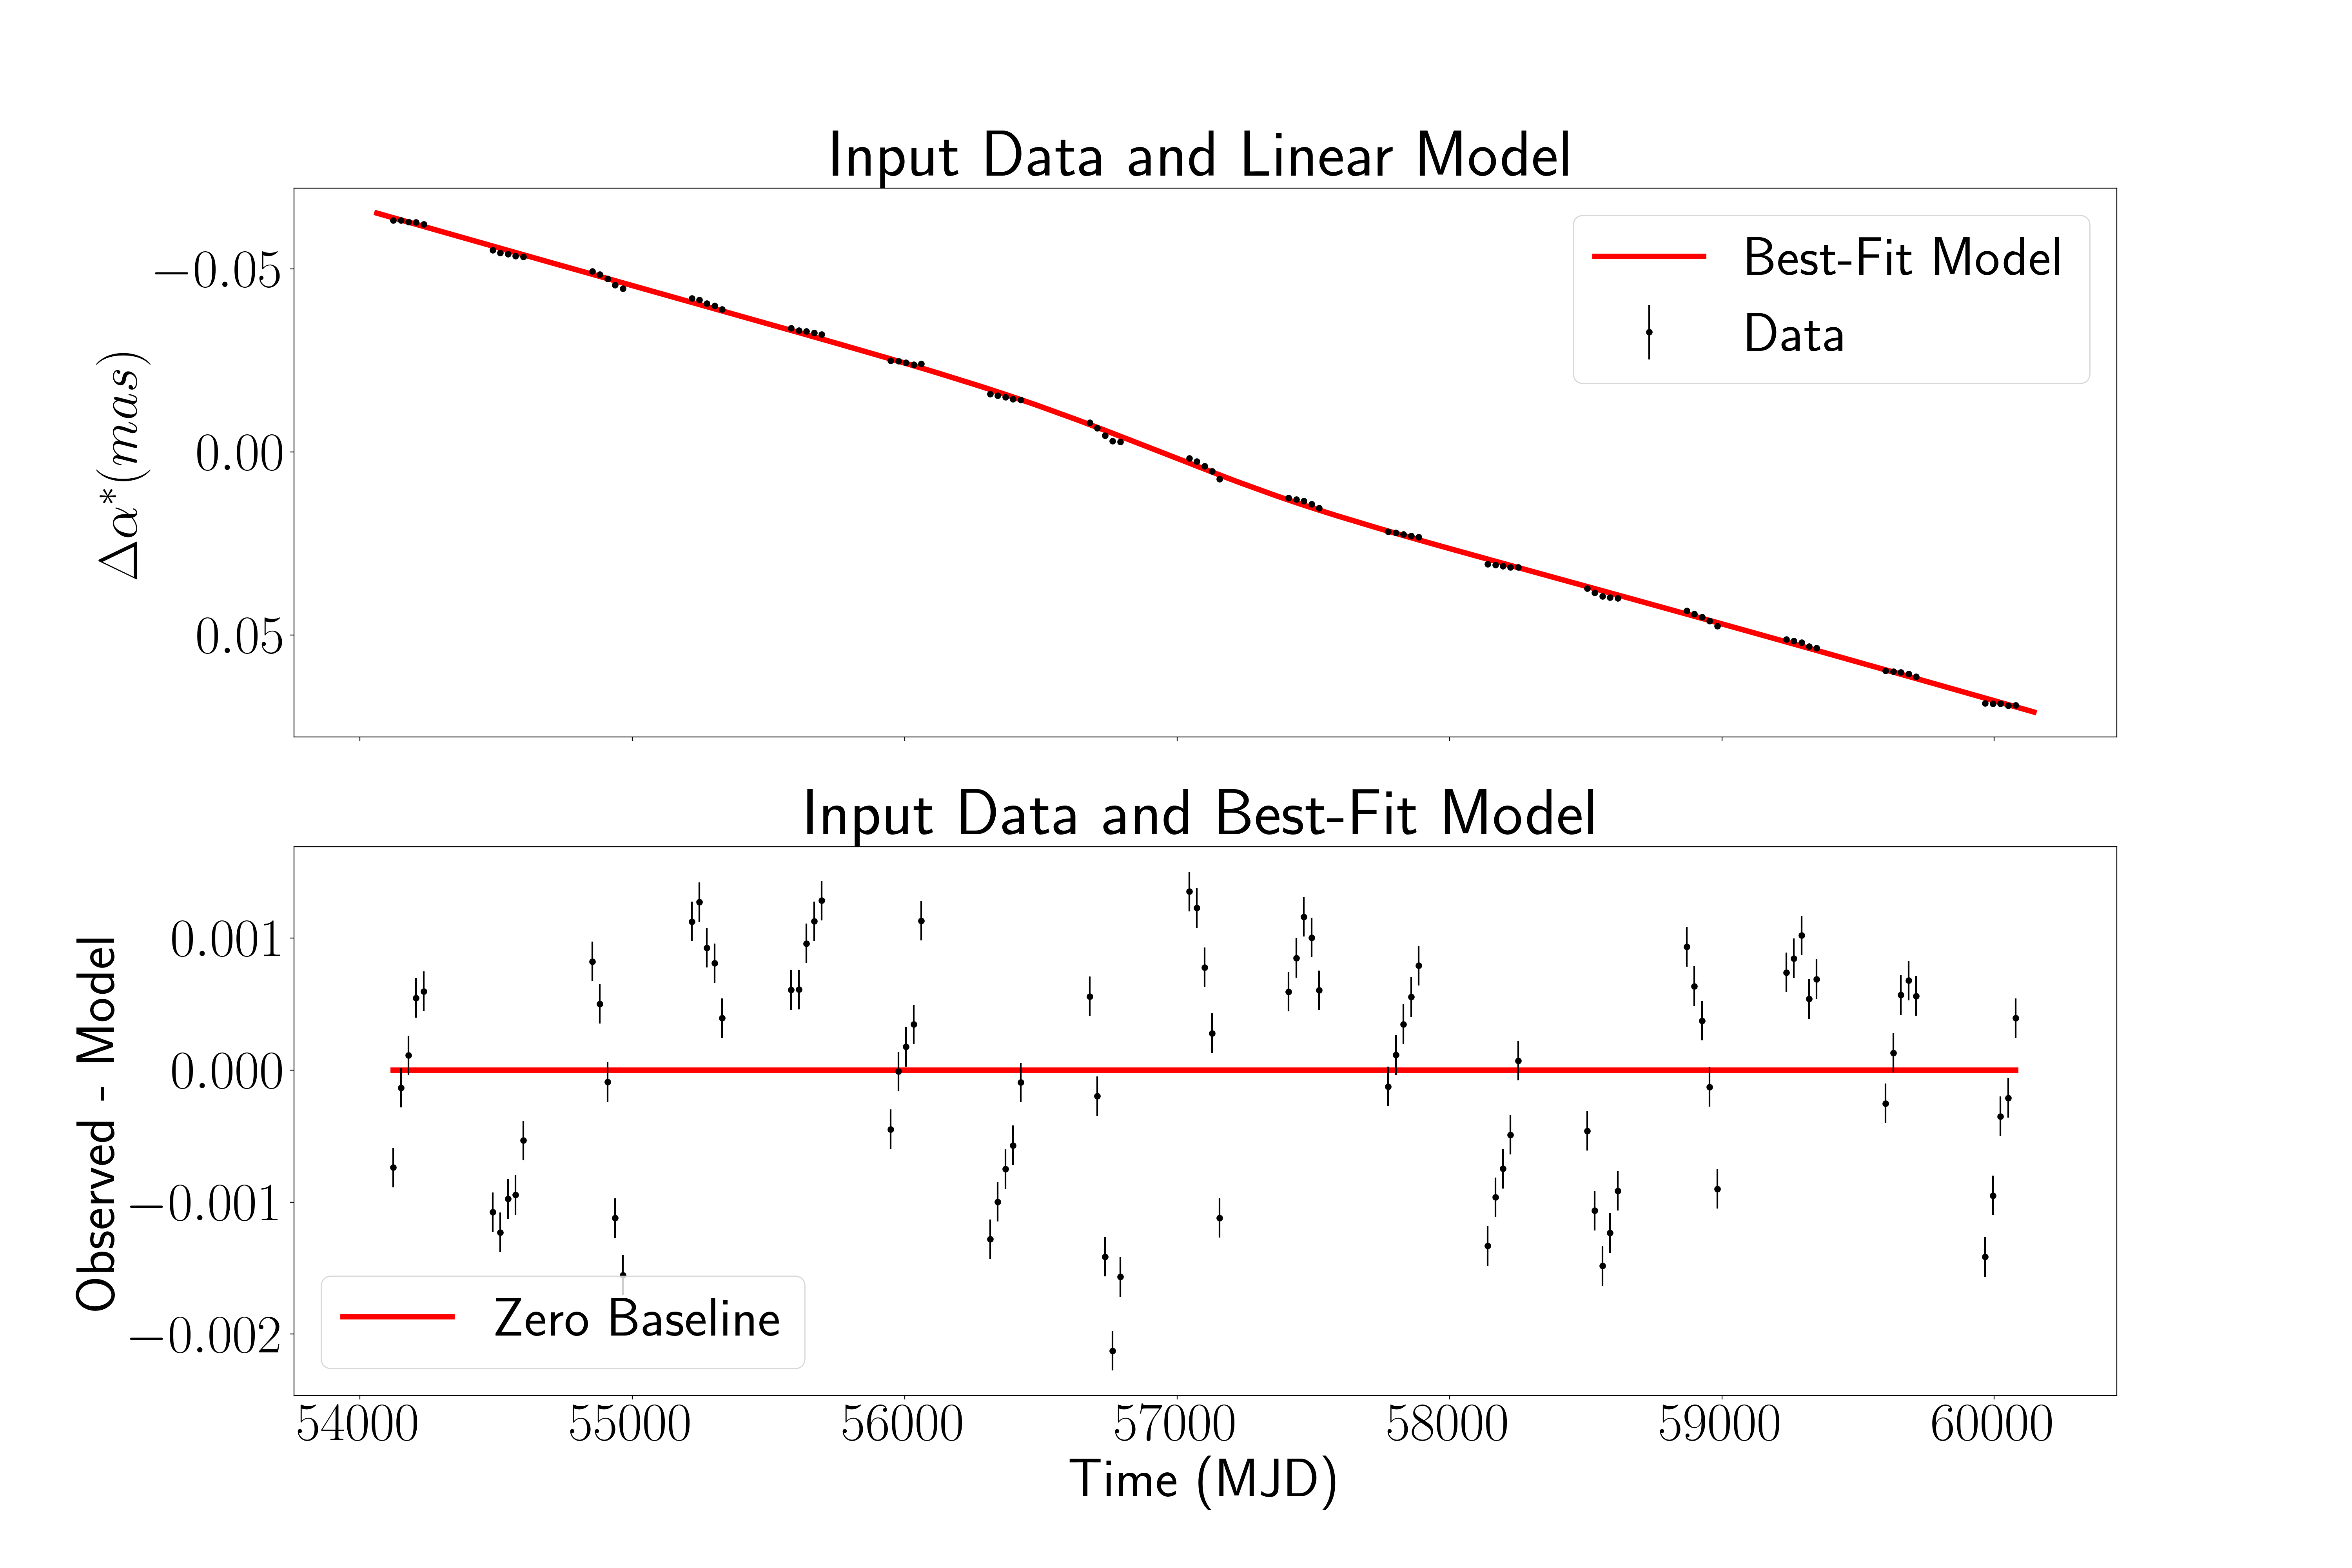
\includegraphics[width= .48 \textwidth]{figures/LinAnalAst1.png}
    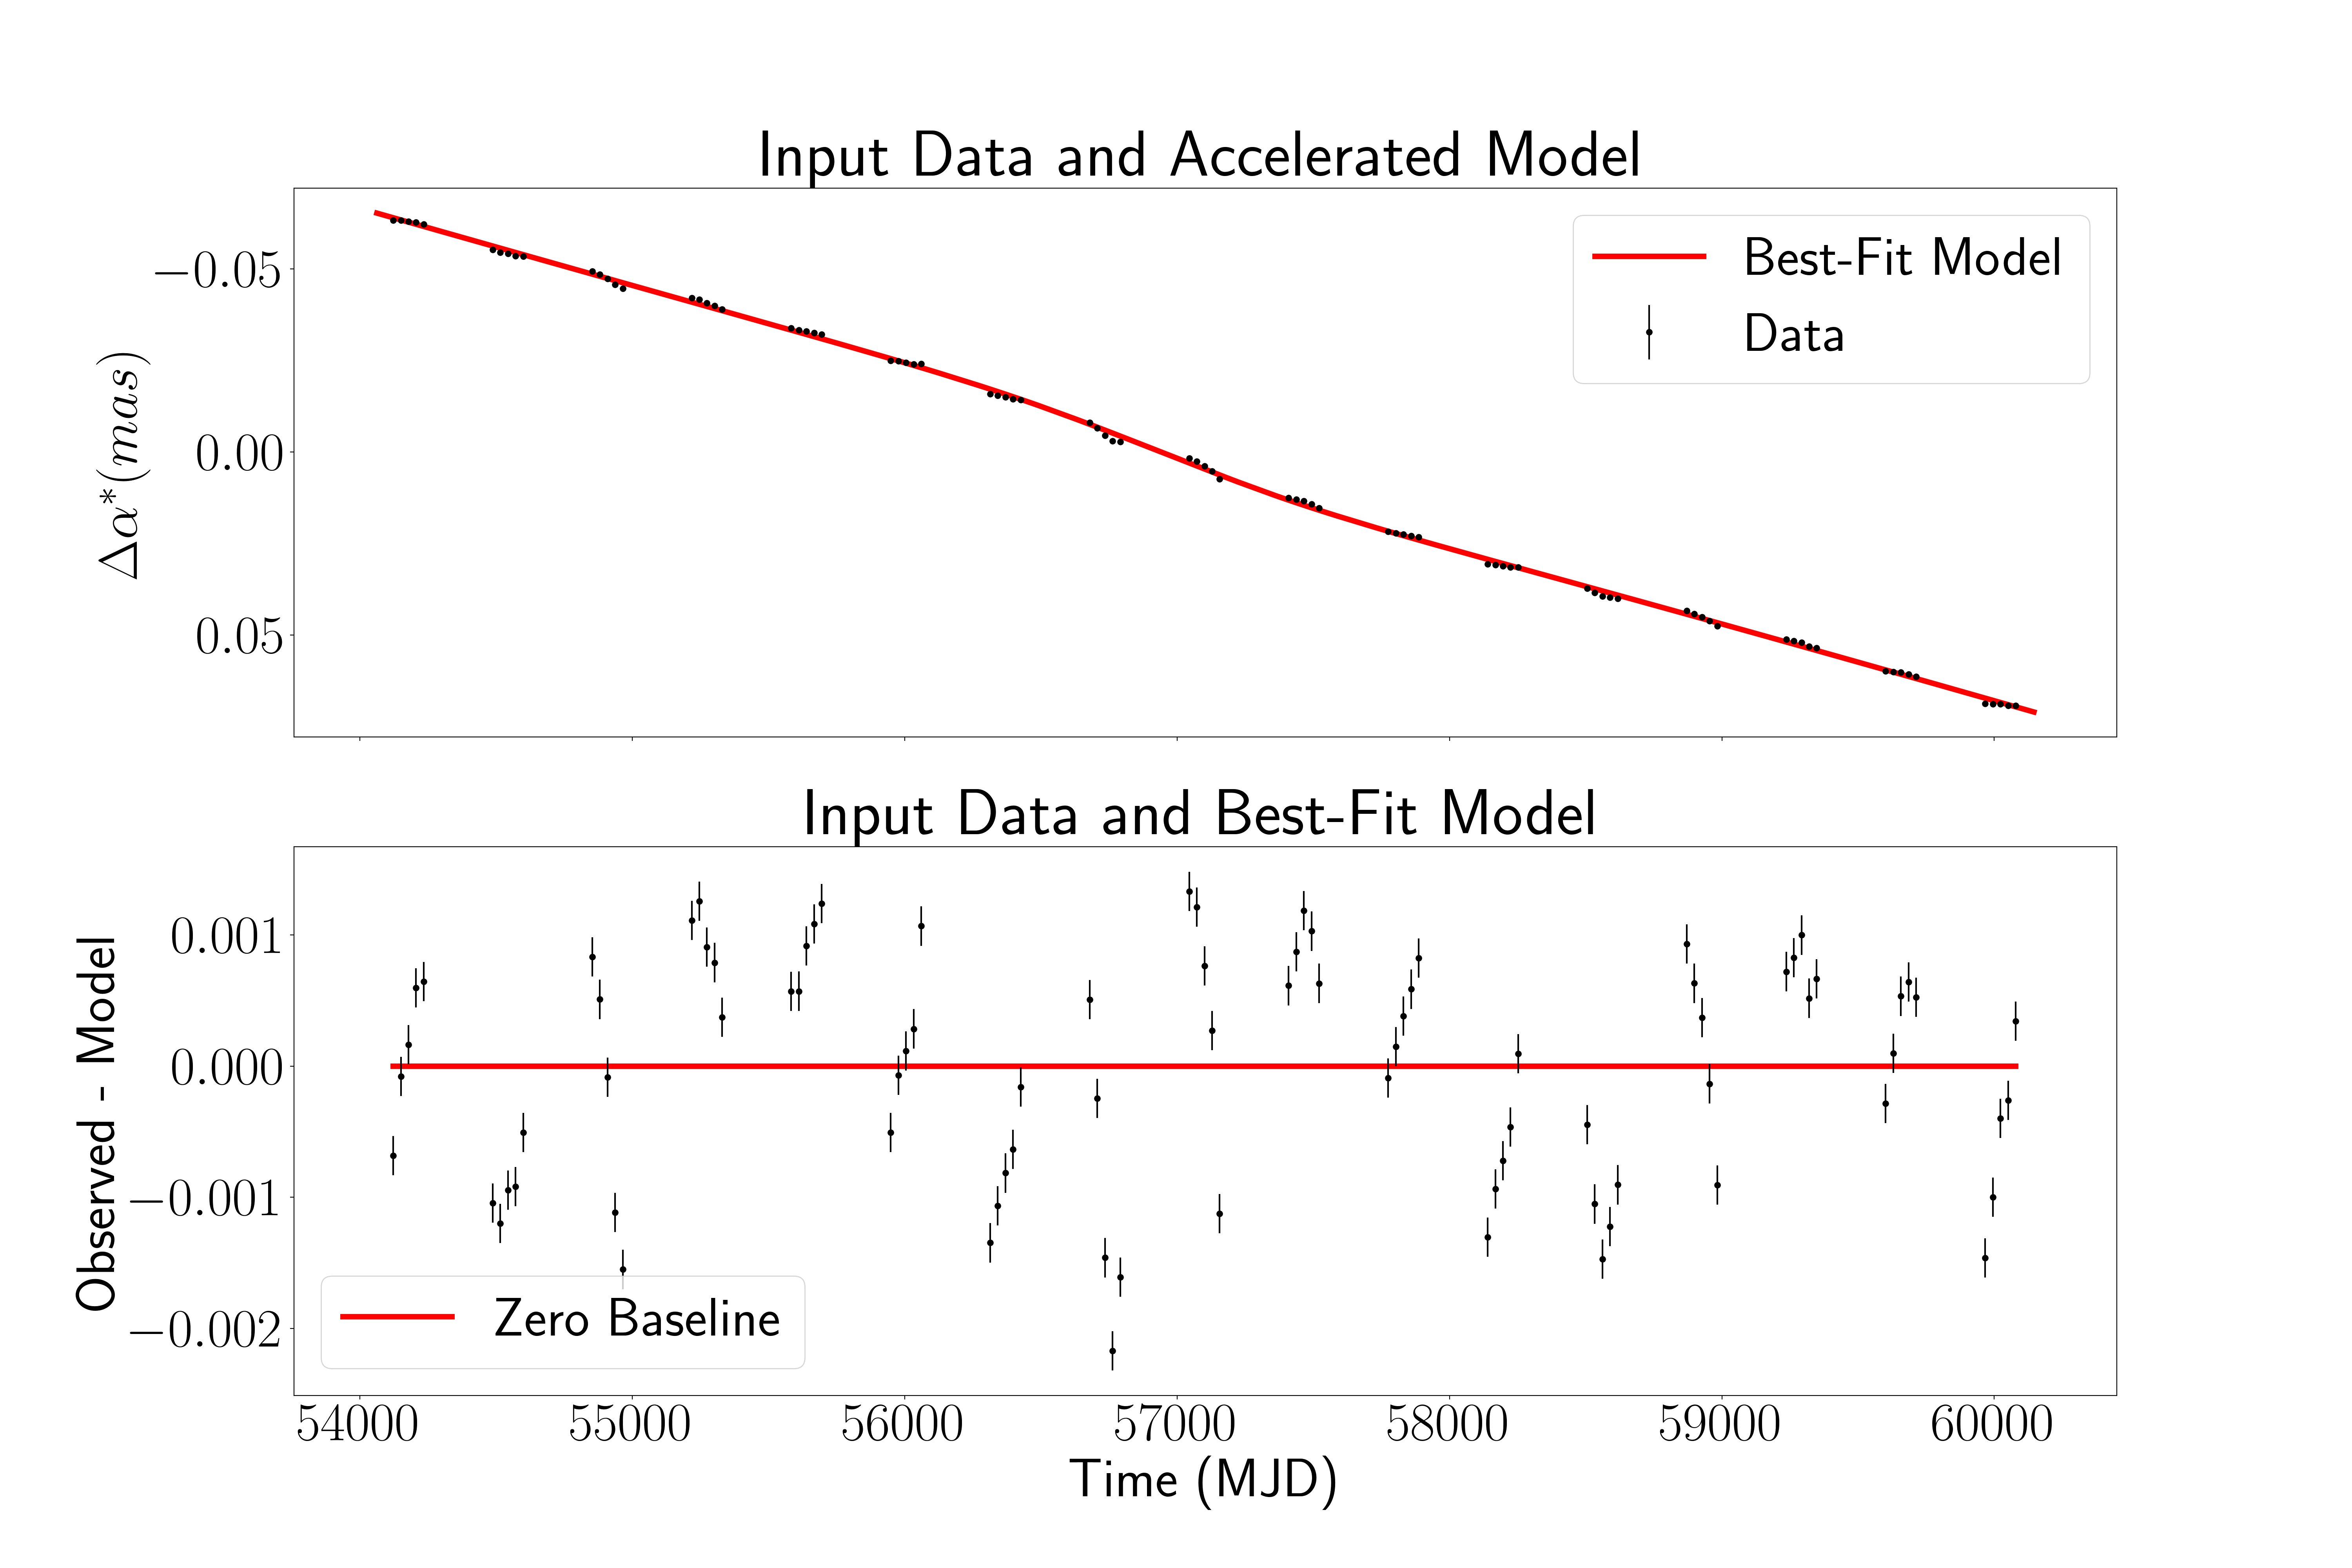
\includegraphics[width= .48 \textwidth]{figures/AccAnalAst1.png}
    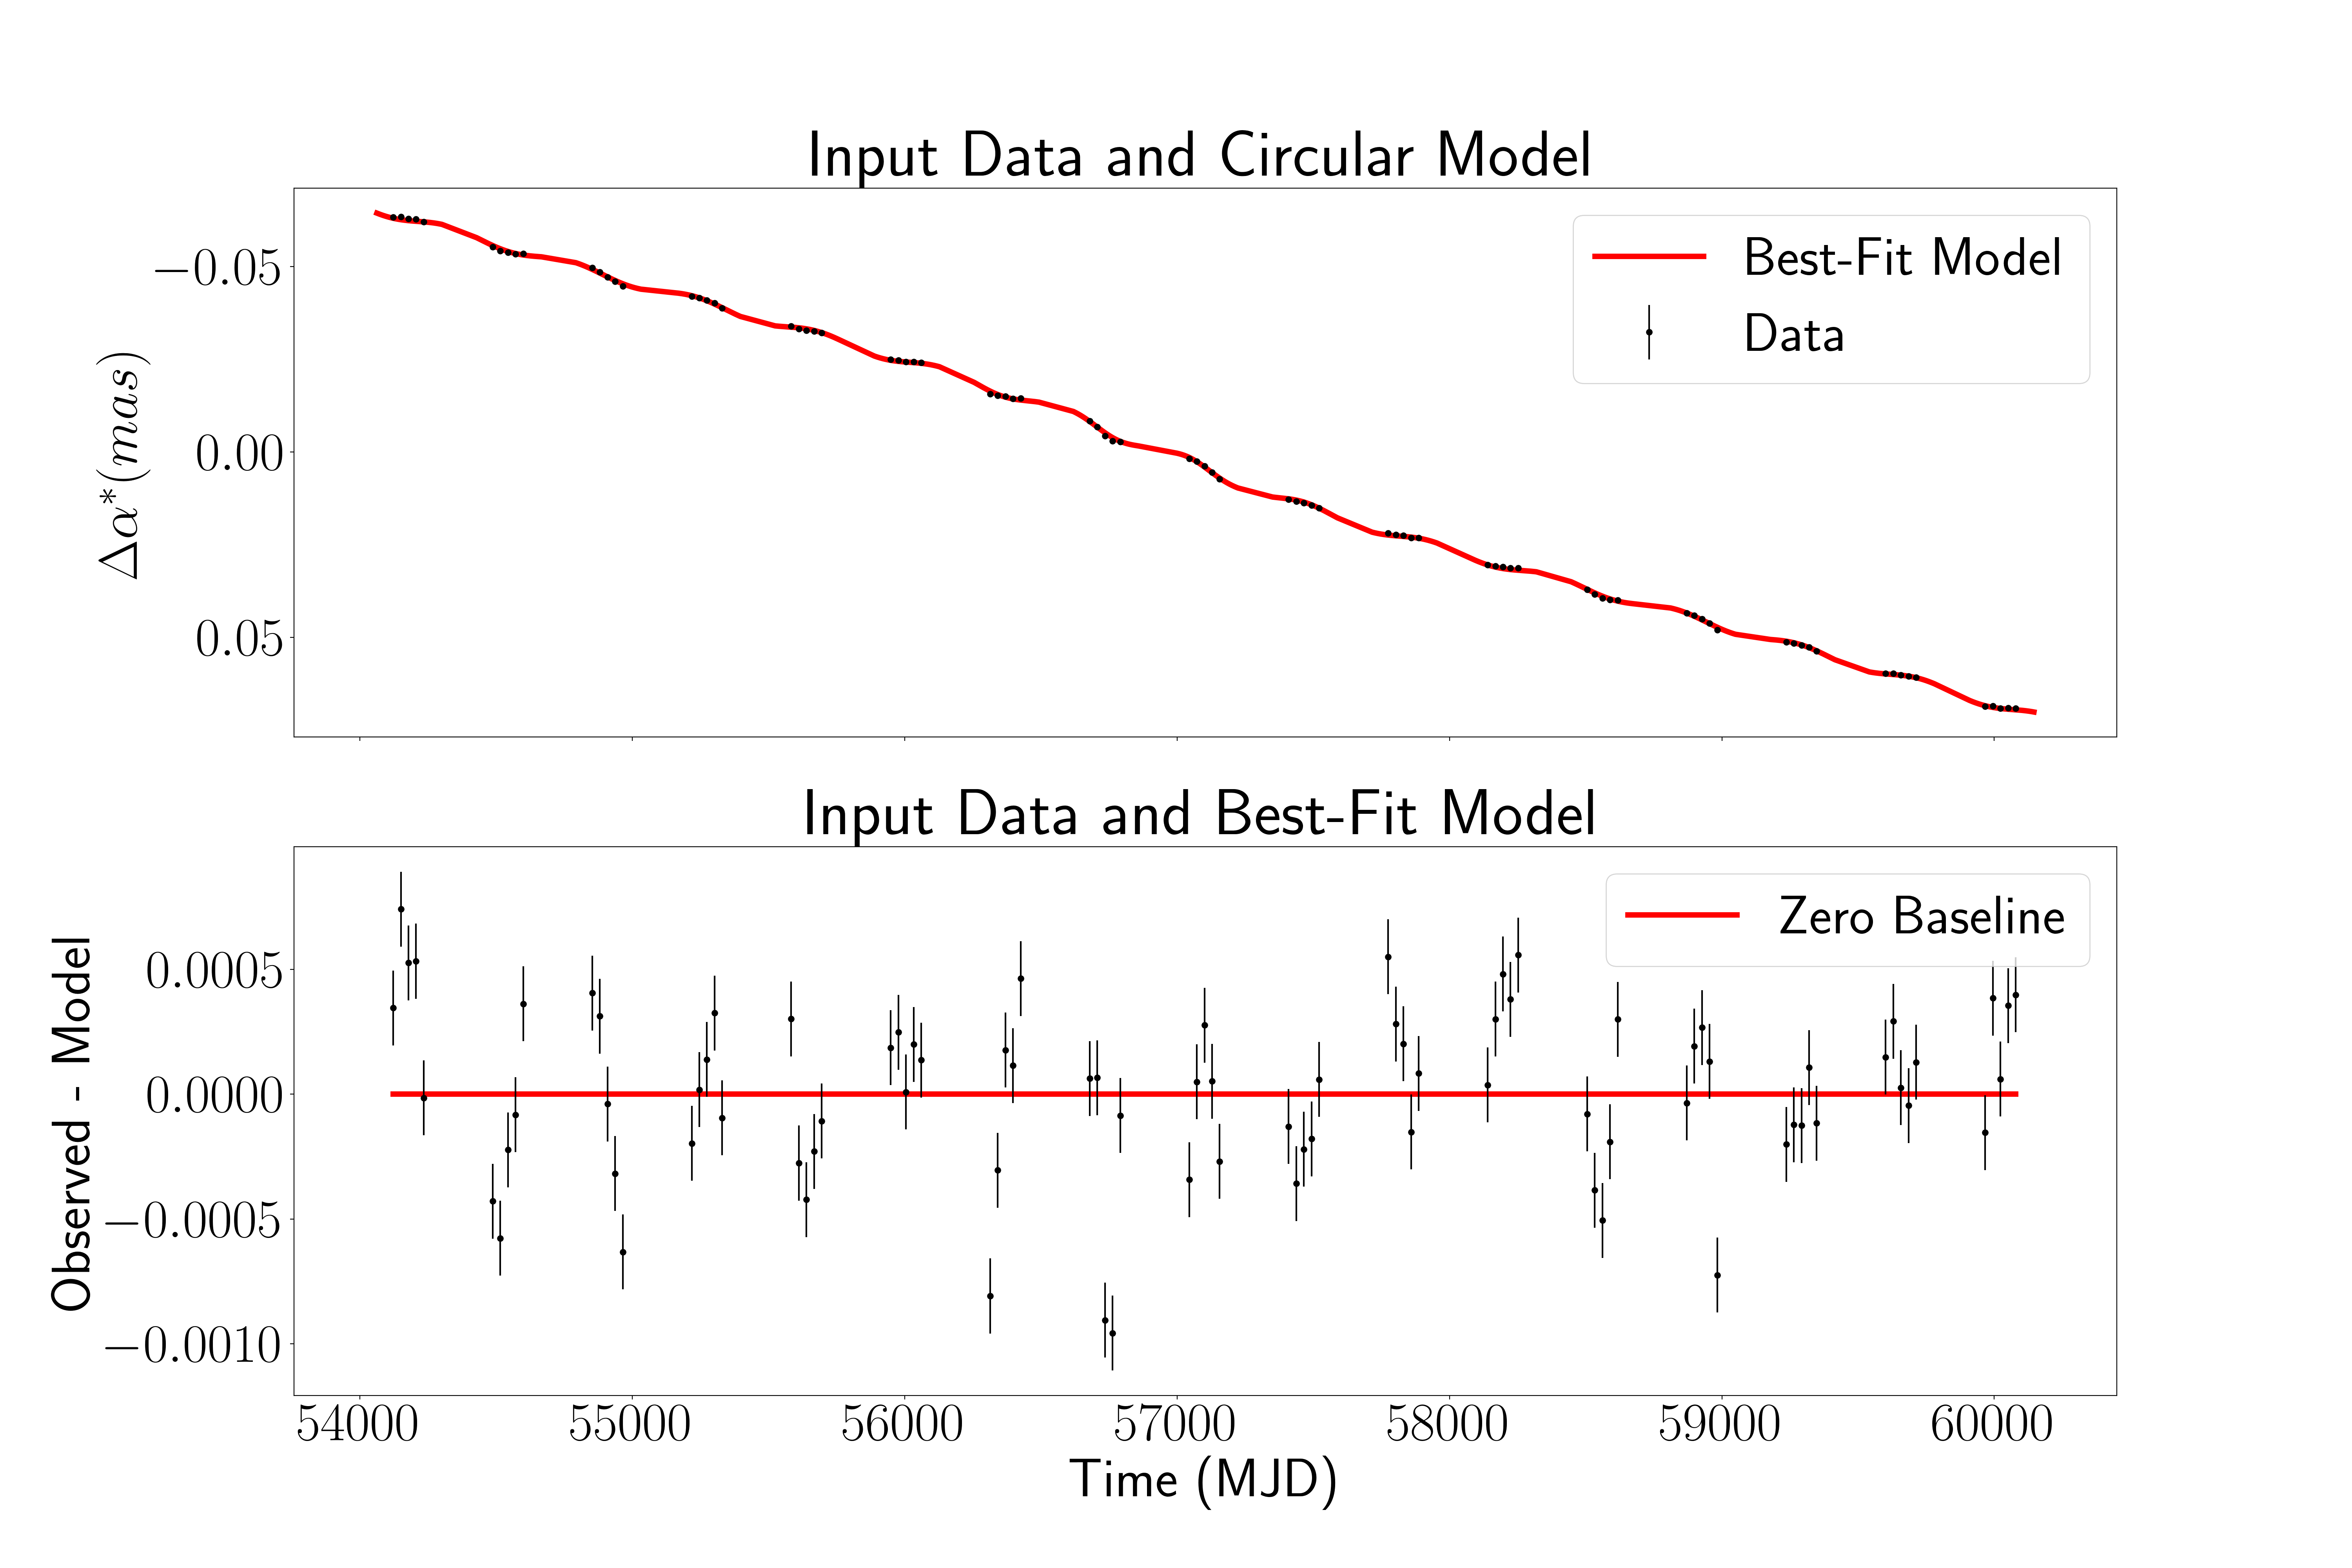
\includegraphics[width= .48\textwidth]{figures/CircAnalAst1.png}
    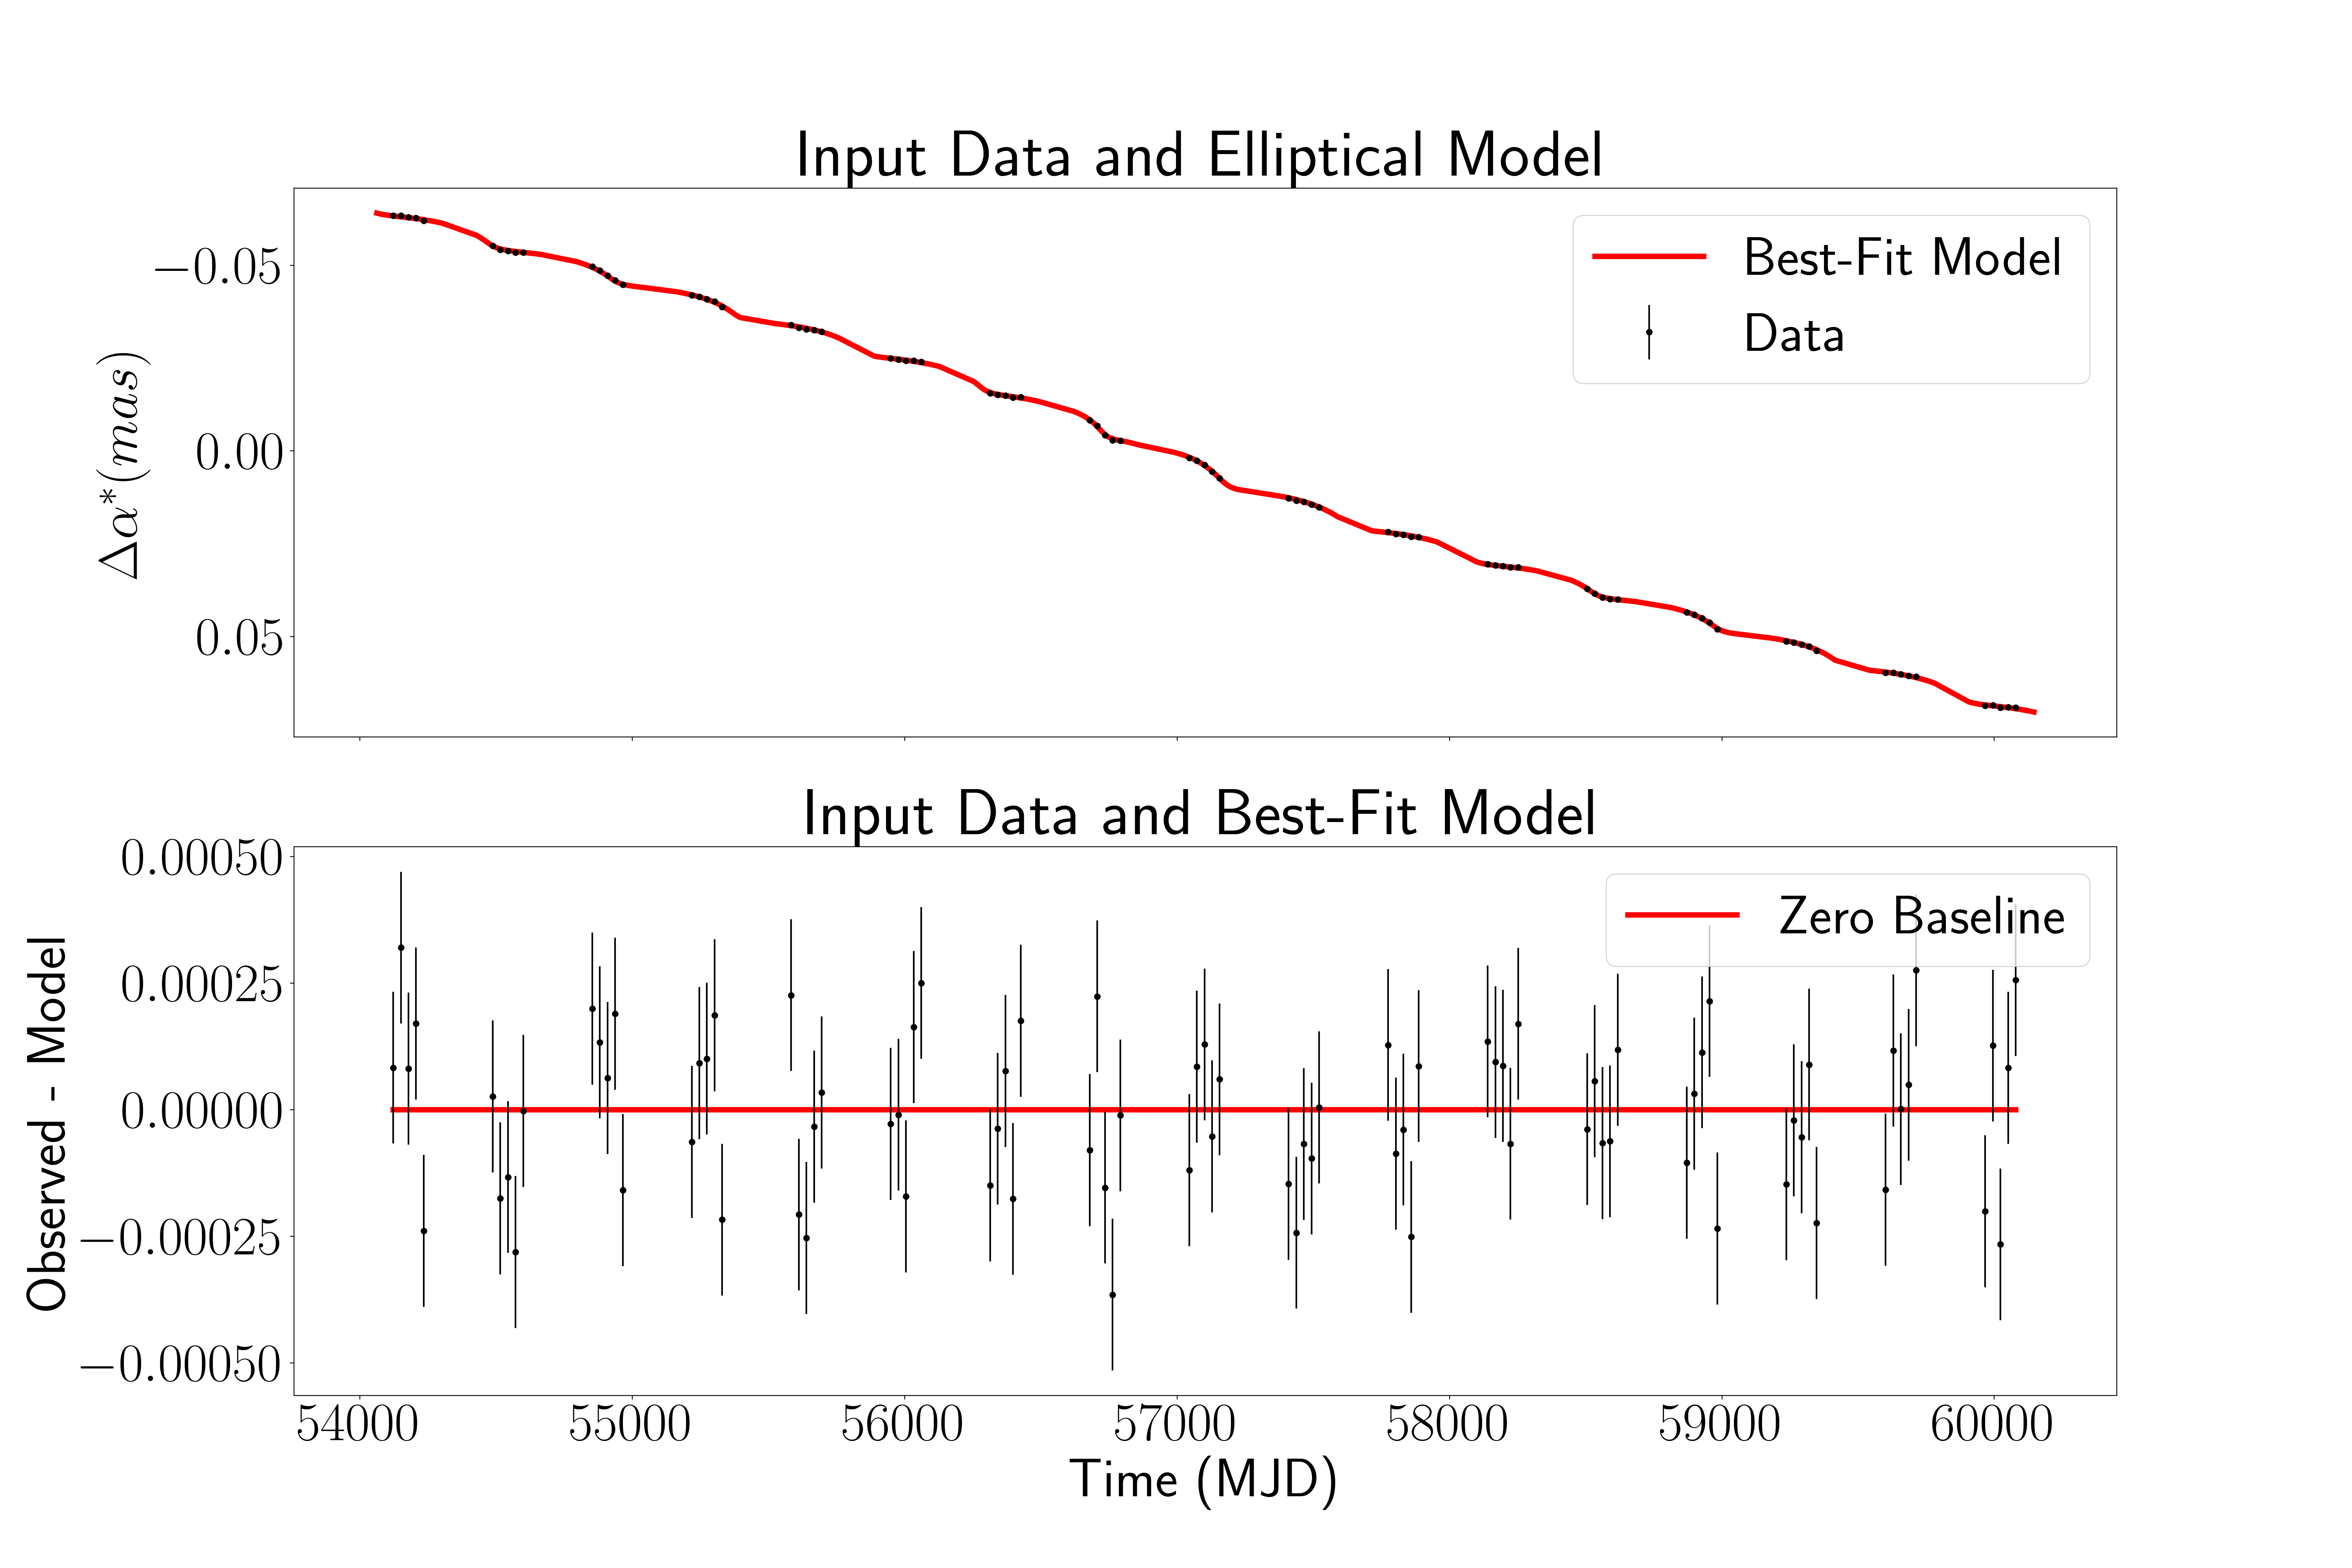
\includegraphics[width= .48\textwidth]{figures/EllAnalAst1.png}

    \caption{Fitting output for a mock astrometric dataset generated using  BSPL\_PhotAstrom\_noPar\_EllOrbs\_Param1 and the parameters displayed in \autoref{tab:fake_fit}. We present a fit for the RA component in this figure. 
    (\emph{Top Left}) Best-fit with linear orbital motion. (\emph{Top Right}) Best-fit with accelerated orbital motion. (\emph{Bottom Left}) Best-fit with circular orbital motion. (\emph{Bottom Right}) Best-fit with elliptical orbital motion}
    \label{fig:orbital_comparison_as1}
\end{figure*}


\begin{figure*}
    \centering
    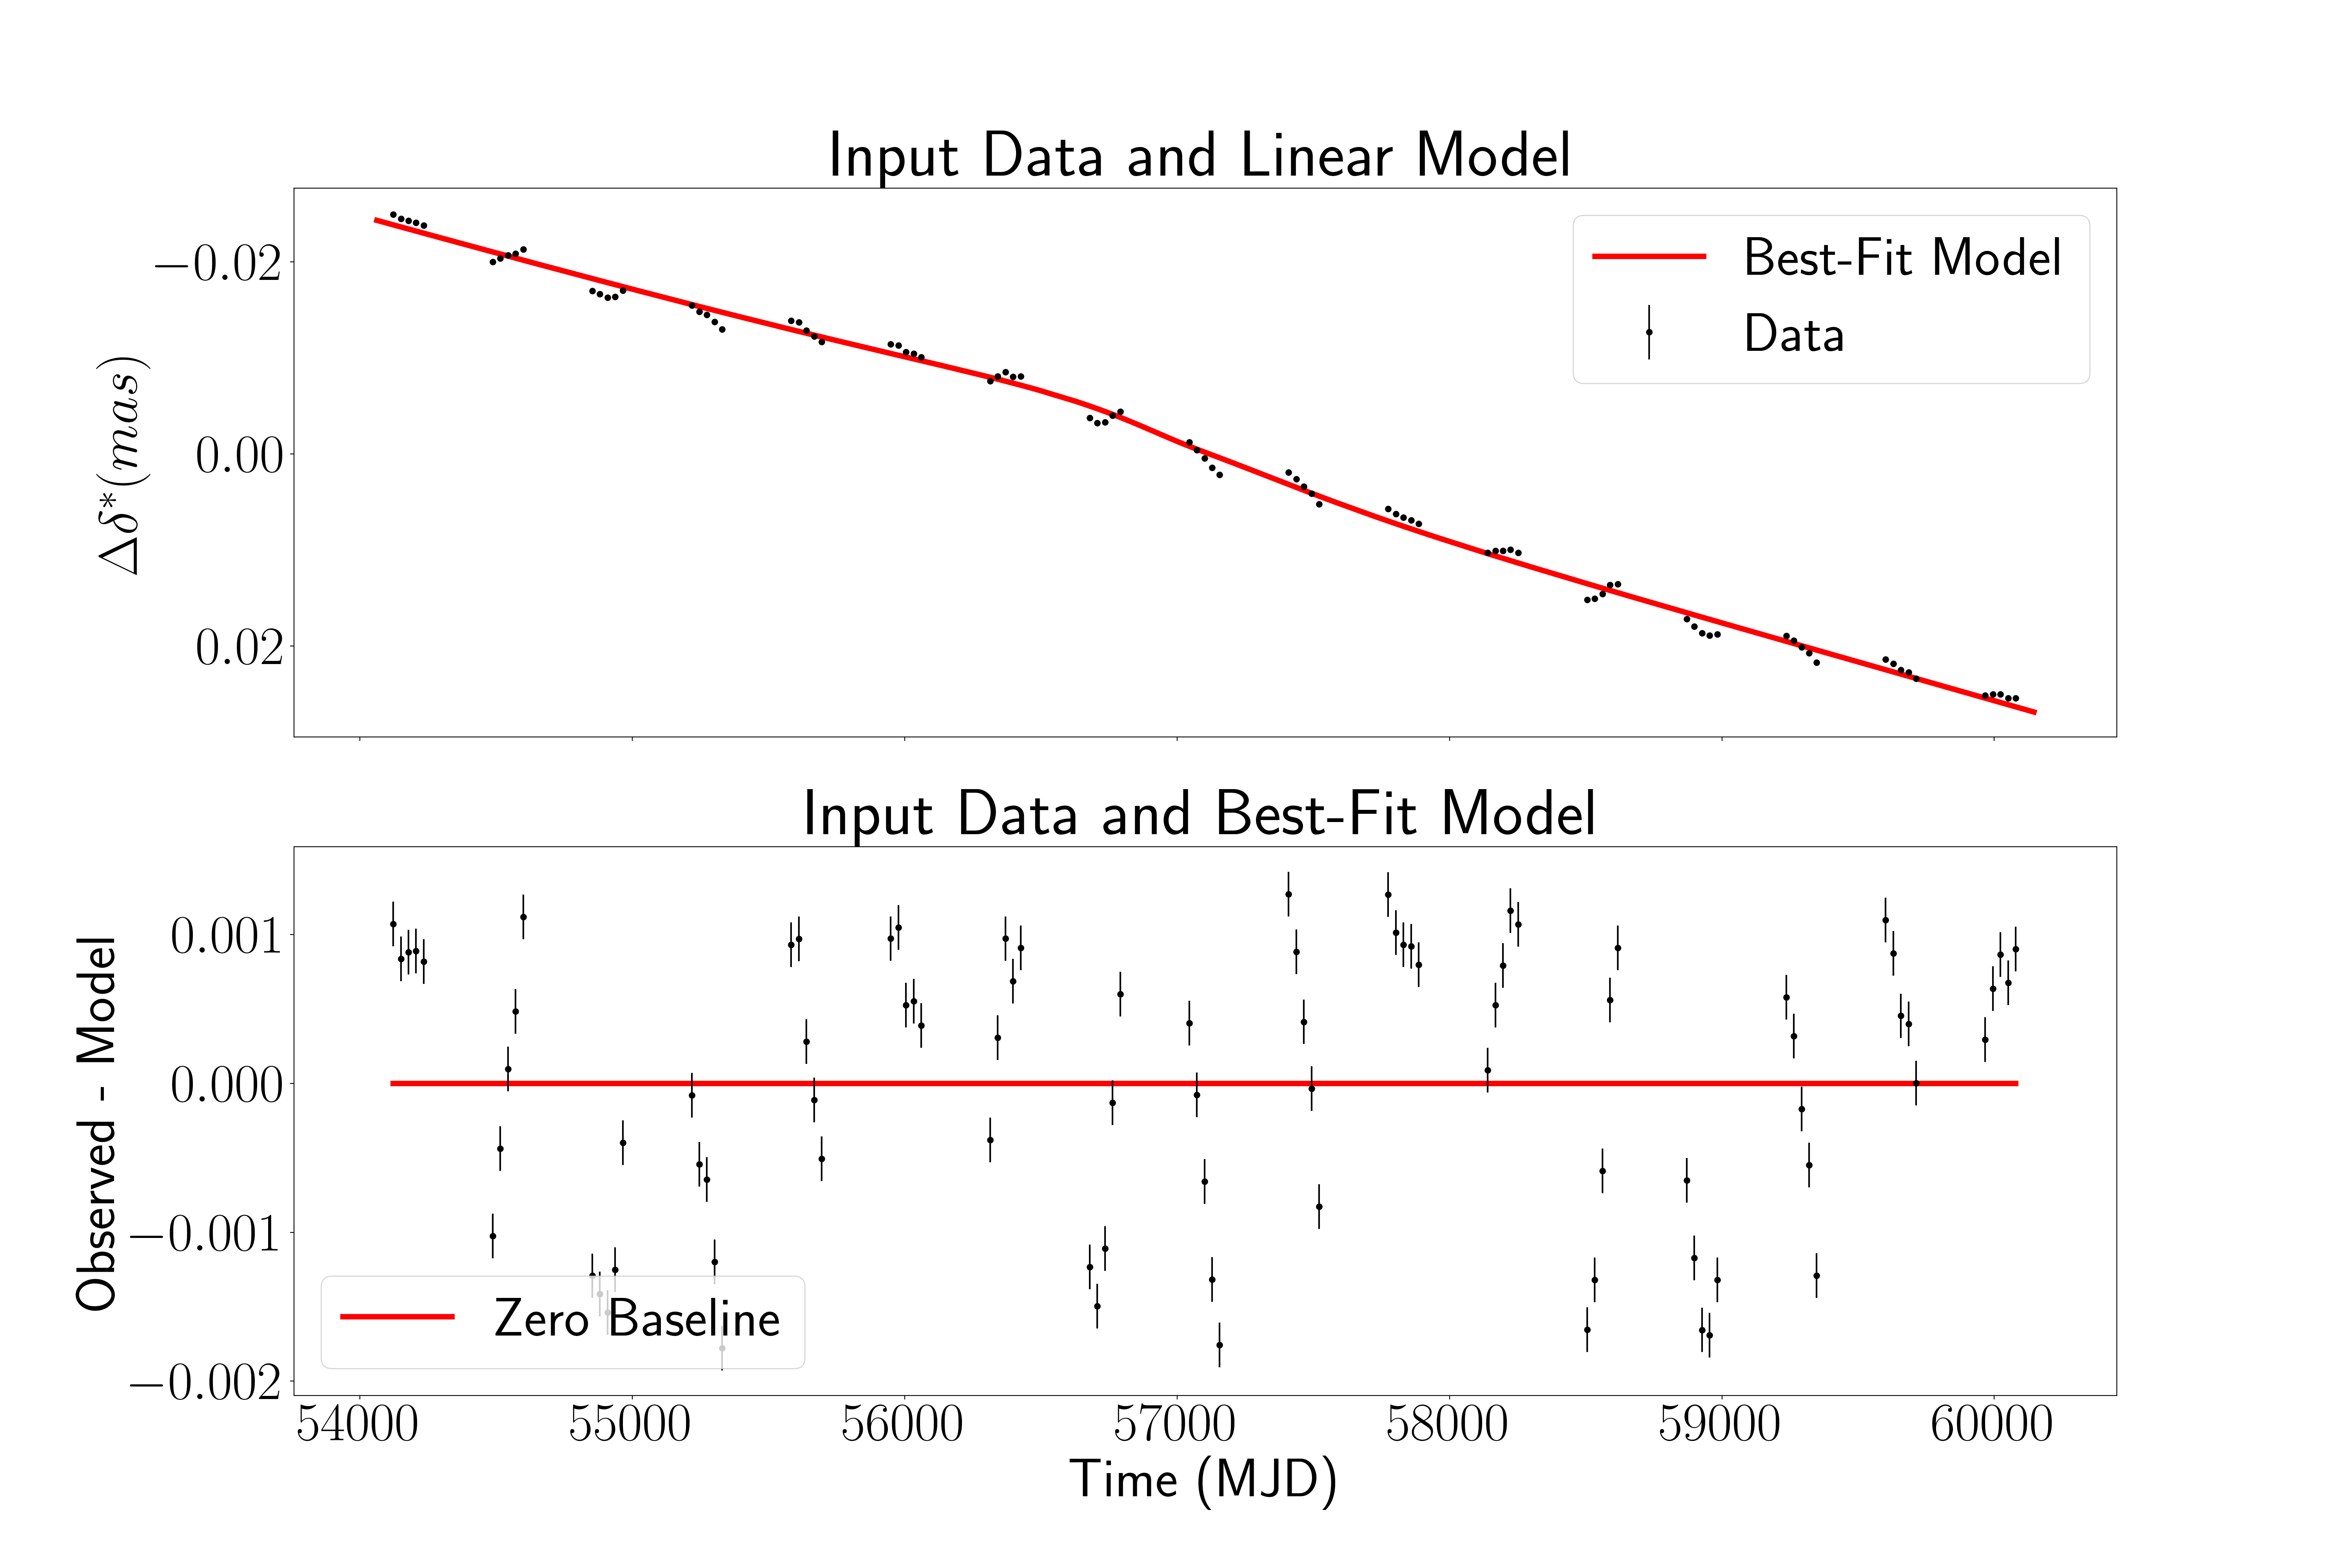
\includegraphics[width= .48 \textwidth]{figures/LinAnalAst2.png}
    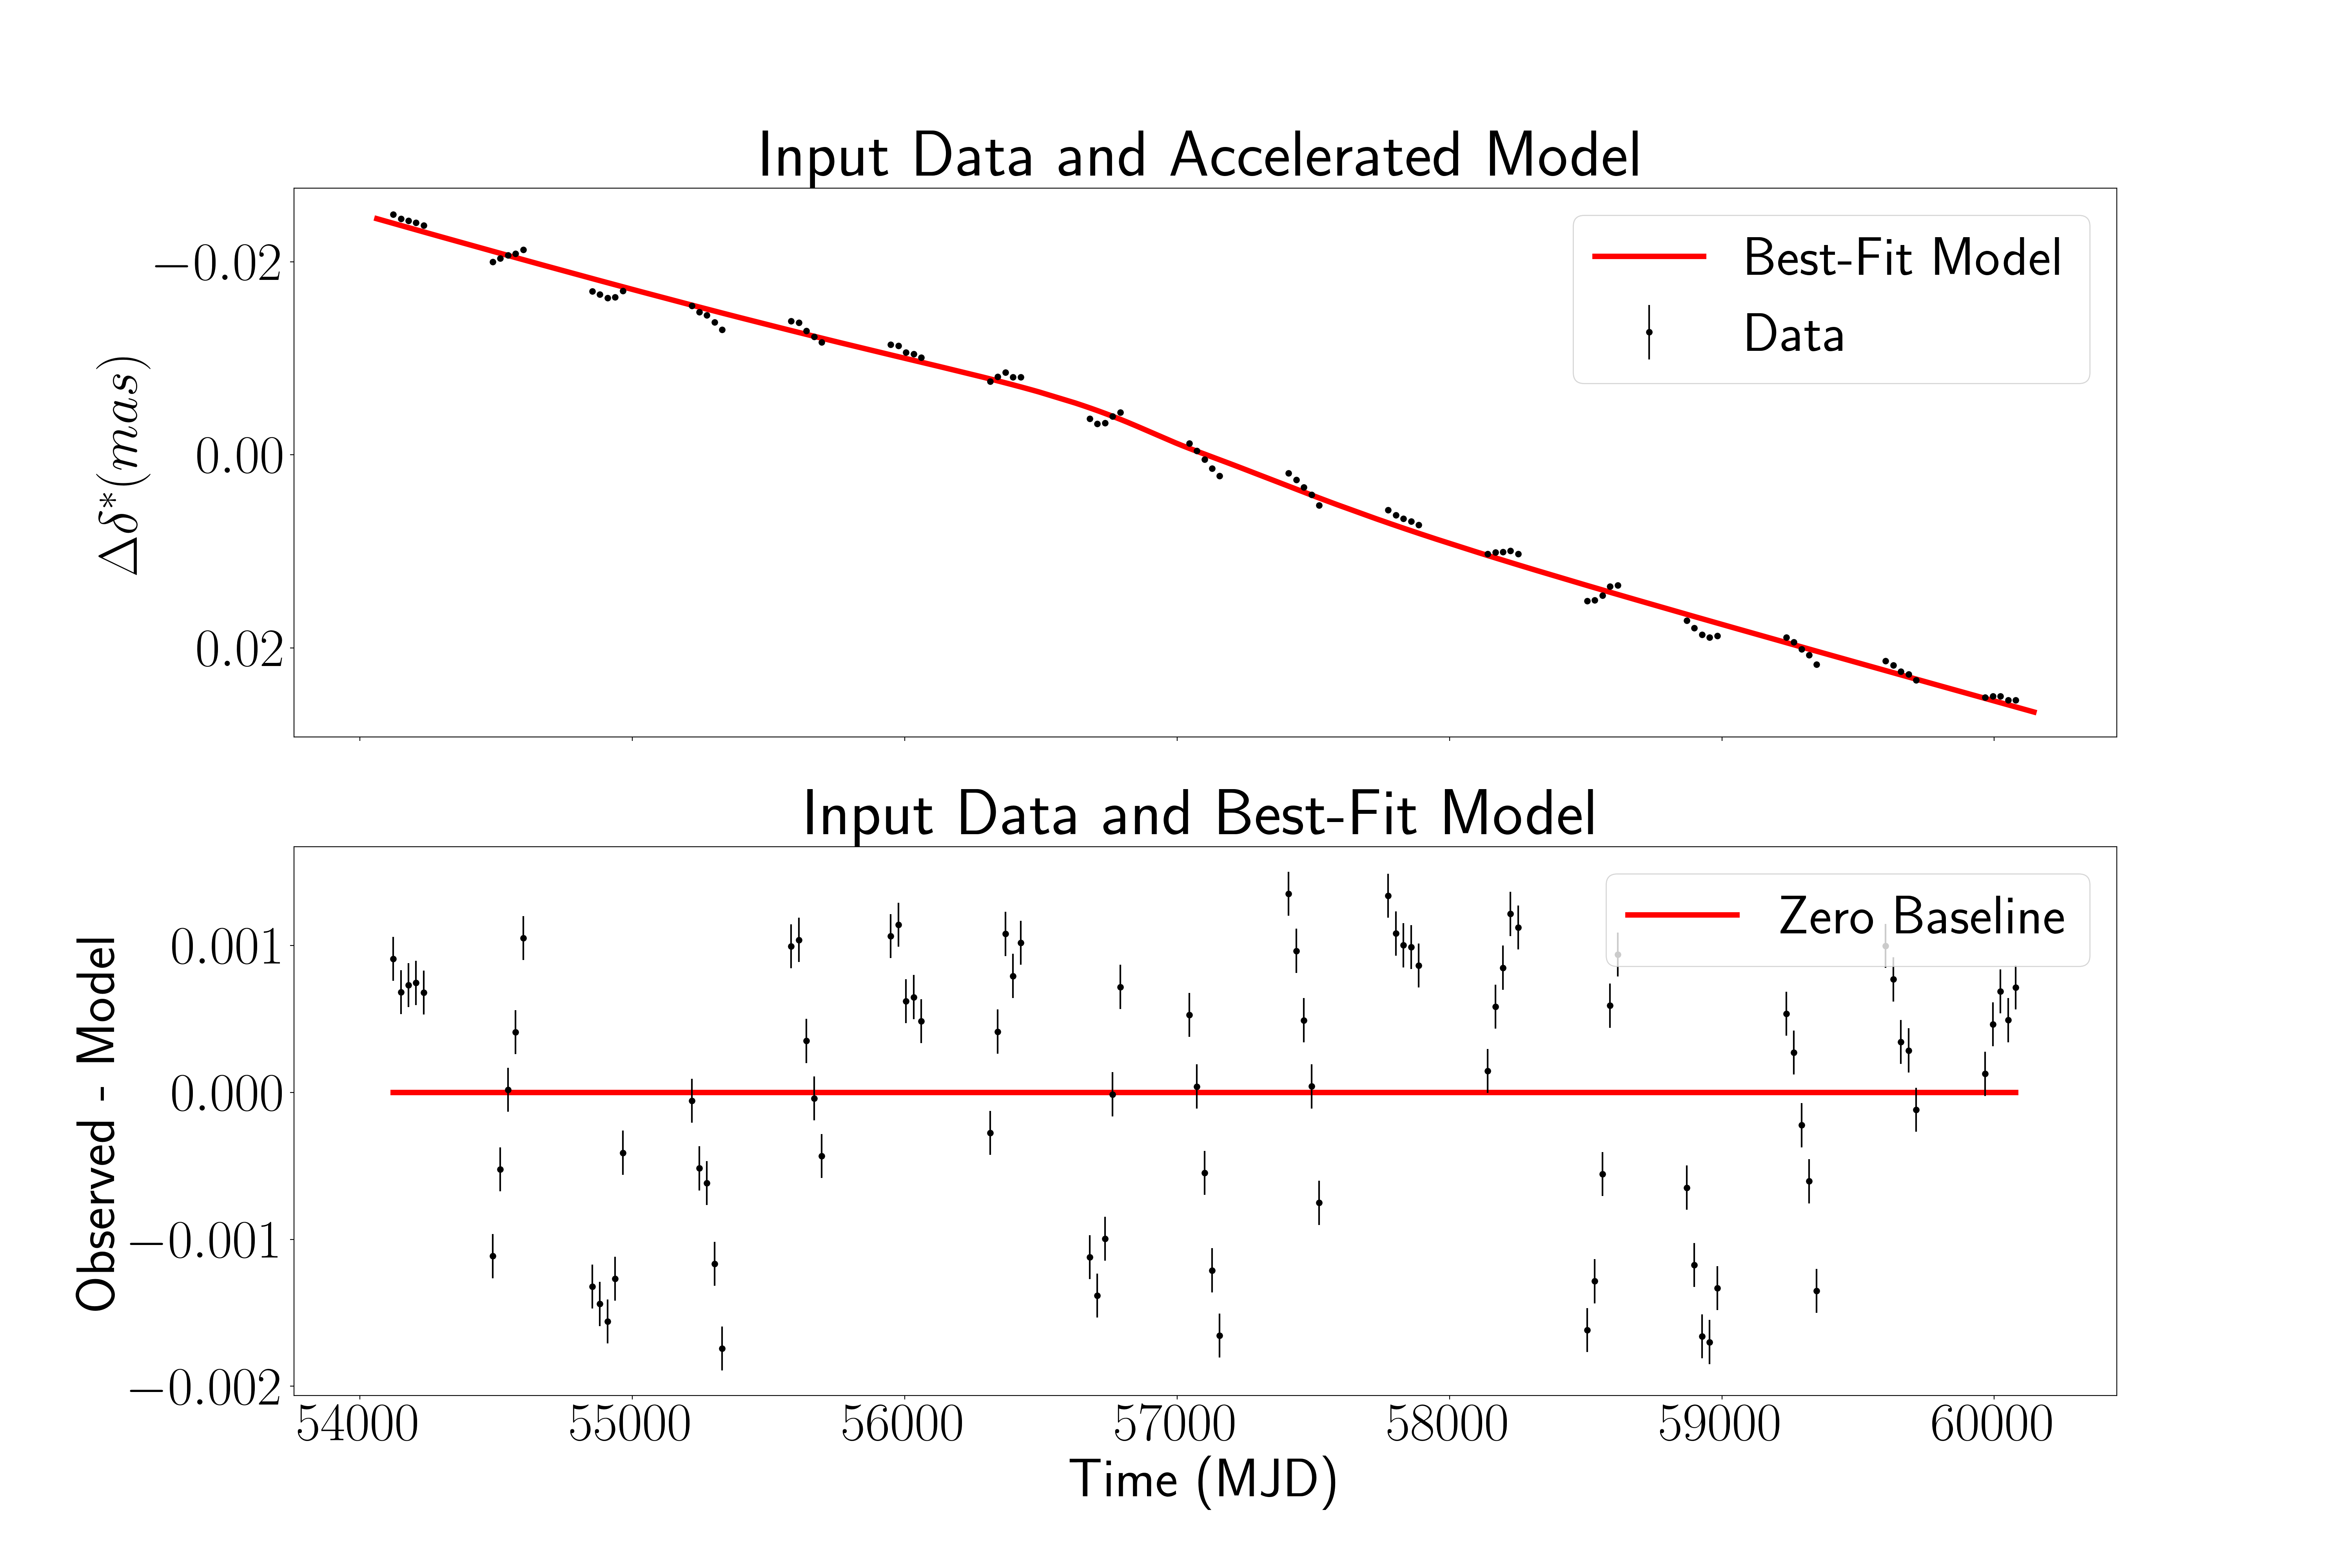
\includegraphics[width= .48 \textwidth]{figures/AccAnalAst2.png}
    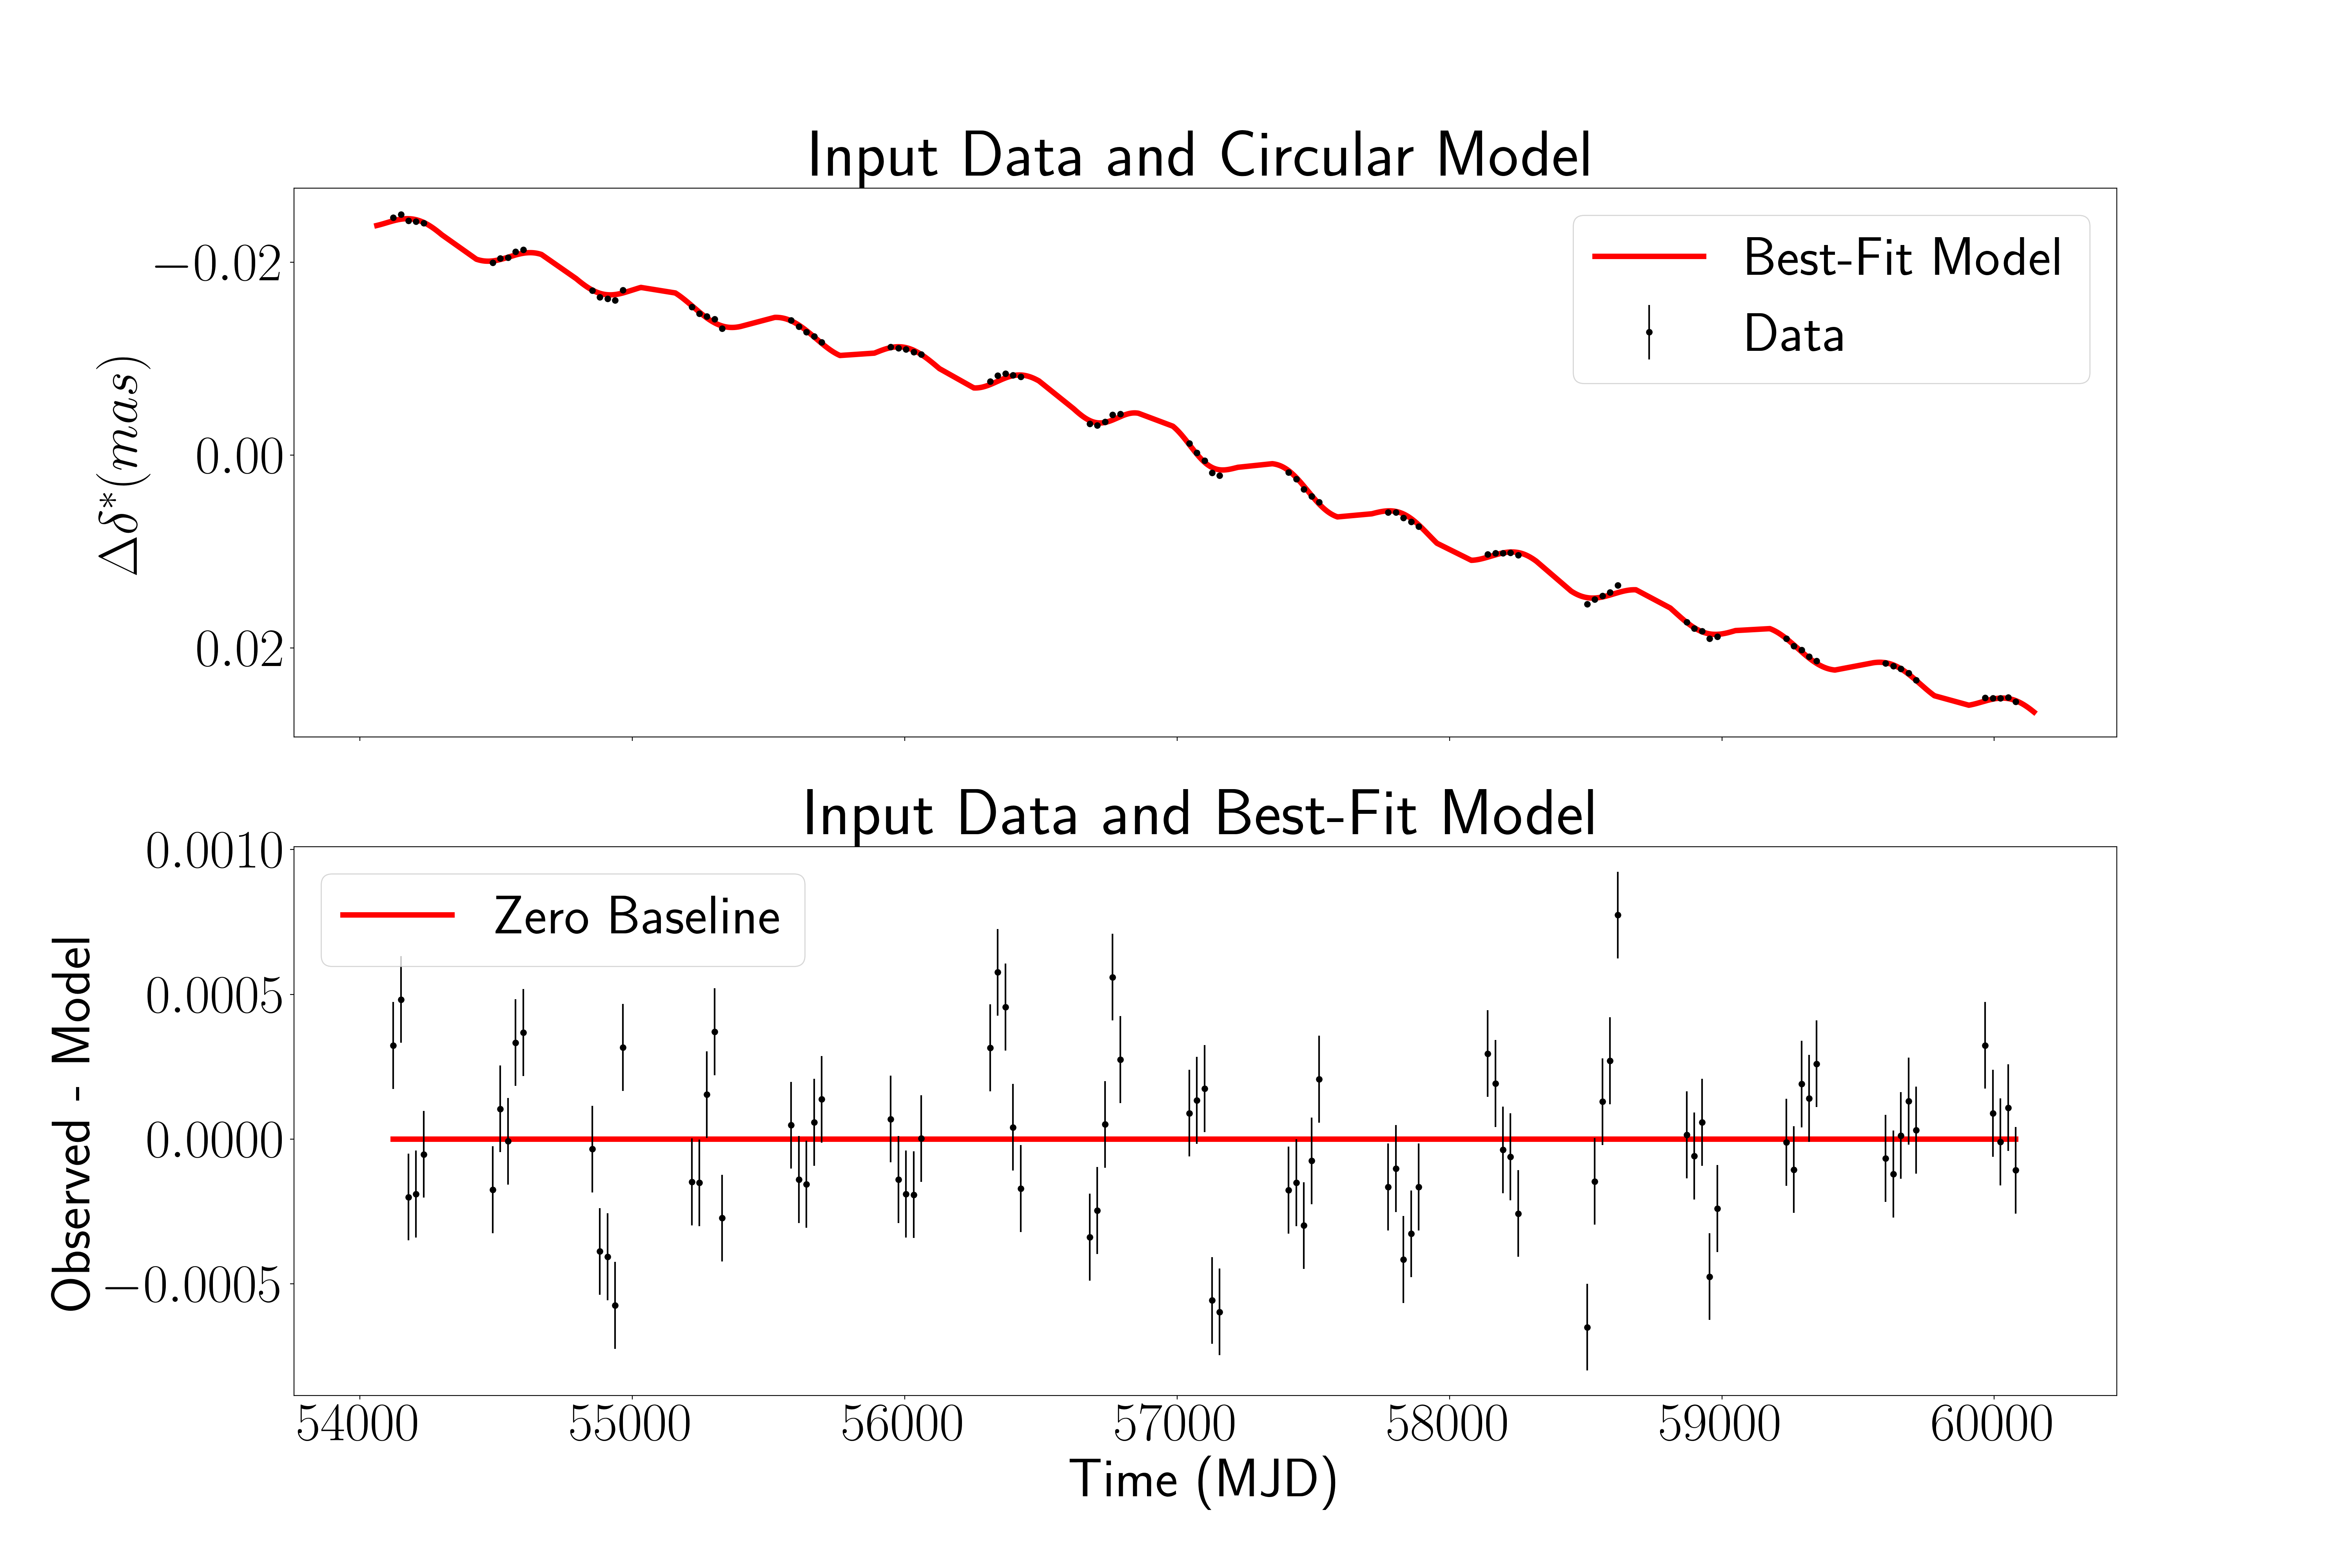
\includegraphics[width= .48\textwidth]{figures/CircAnalAst2.png}
    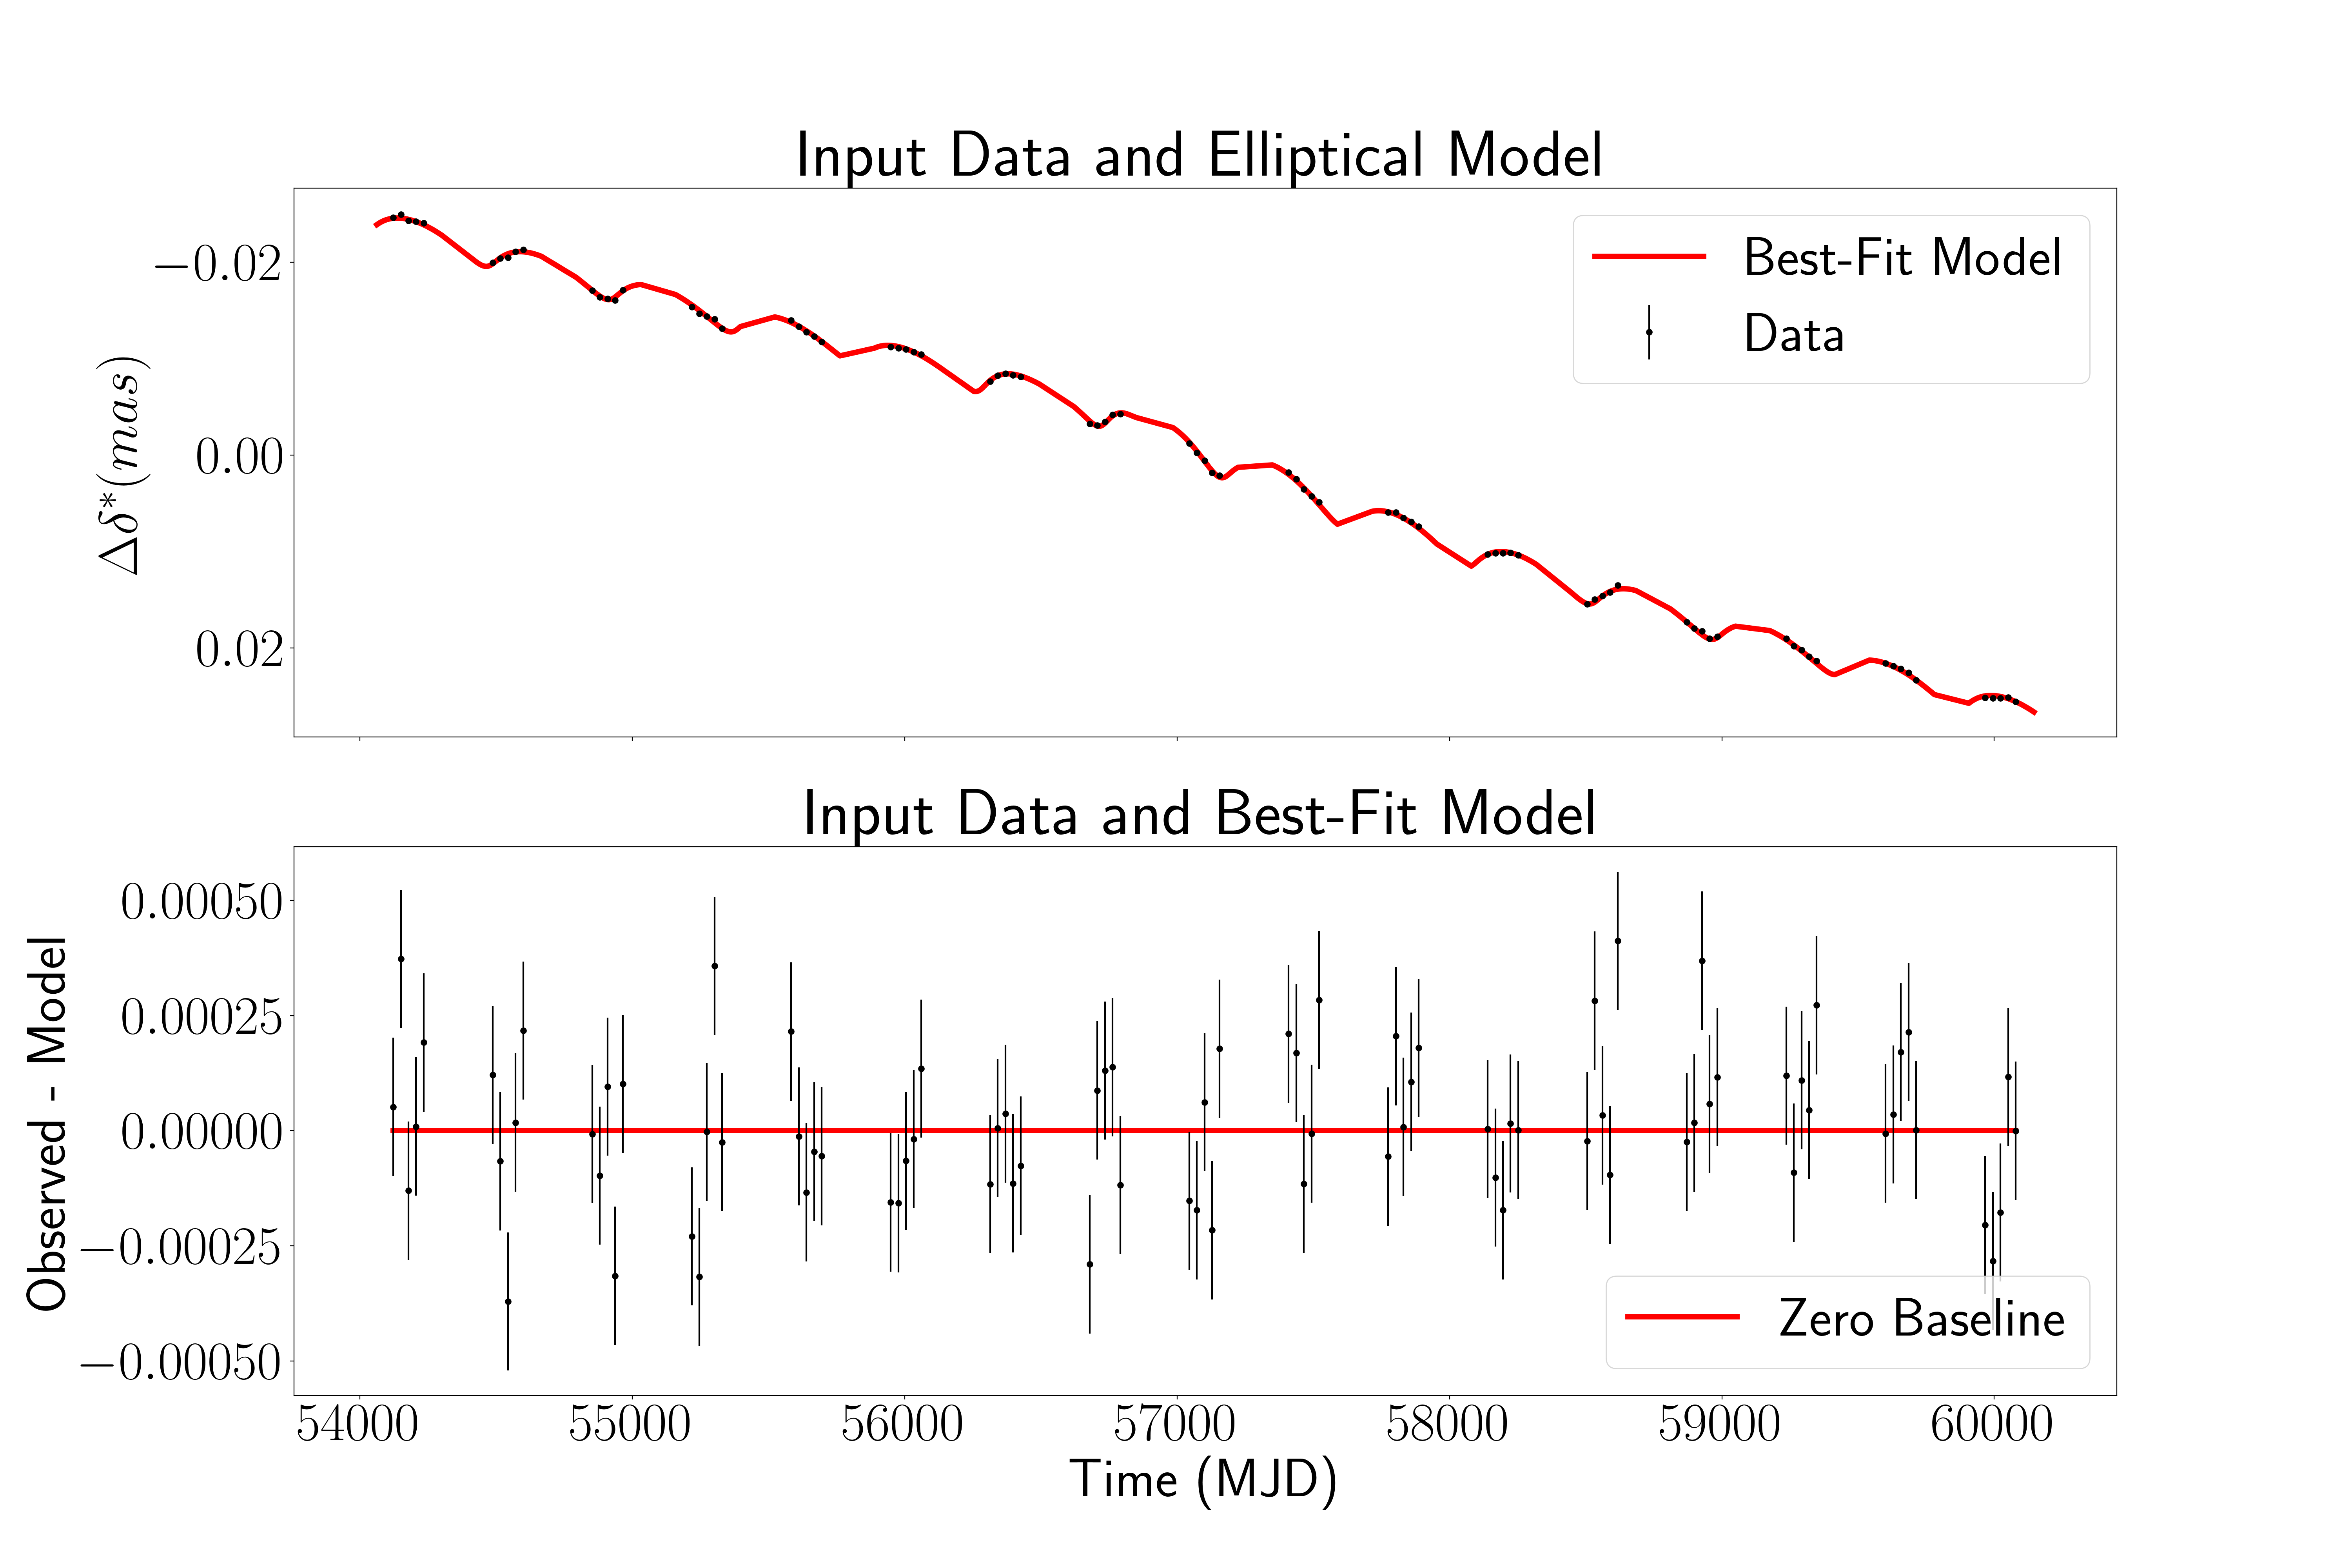
\includegraphics[width= .48\textwidth]{figures/EllAnalAst2.png}

    \caption{Fitting output for a mock astrometric dataset generated using  BSPL\_PhotAstrom\_noPar\_EllOrbs\_Param1 and the parameters displayed in Table ~\ref{tab:fake_fit}. We present a fit for the RA component in this figure. 
    (\emph{Top Left}) Best-fit with linear orbital motion. (\emph{Top Right}) Best-fit with accelerated orbital motion. (\emph{Bottom Left}) Best-fit with circular orbital motion. (\emph{Bottom Right}) Best-fit with elliptical orbital motion}
    \label{fig:orbital_comparison_as2}
\end{figure*}


\subsection{Results: Orbital Motion}
\label{sec:results_om}



In this section, we demonstrate the need to account for the orbital motion of binary systems by fitting a mock dataset to various models with orbital motion in BAGLE. 

The mock dataset generated is intentionally designed to replicate a BSPL event with a complex lightcurve structure with apparent Keplerian motion. It is generated using BSPL\_PhotAstrom\_noPar\_EllOrbs\_Param1 and the parameters presented in Table~\ref{tab:fake_fit}. The mock dataset simulates photometric observations every day and astrometric observations every twenty-eight days for the bulge observing window. In a year, simulated observations are missed for 125 days for photometry and 165 days for astrometry. 

In our fitting process, BSPL models with linear, accelerated, circular, and elliptical orbital motion are utilized to demonstrate how incorporating orbital motion enhances the quality of the fitting process. We present the photometric fitting results in Figure~\ref{fig:orbital_comparison}, the astrometric RA fitting results in Figure~\ref{fig:orbital_comparison_as1} and the astrometric Dec fitting results in Figure~\ref{fig:orbital_comparison_as2}. 

Visually, the residuals improve when fitting a model with either a circular or elliptical orbital motion (as compared to accelerated or linear approximations), which is more closely aligned with the true nature of the mock dataset. 

Furthermore, the reduced chi-squared ($\bar{\chi}^2$) values are summarized in Table~\ref{tab:chi}, and capture the quality of the fits. In our reduced chi-squared test, we calculated the degrees of freedom by subtracting the number of fitting parameters from the total number of astrometric and photometric data points. The best-fit models with linear and accelerated orbital motion have a $\bar{\chi}^2 = 3.214$ and $\bar{\chi}^2 = 3.212$, respectively. The linear and accelerated models overestimate the analytical uncertainties on the dataset. On the other hand, the best fits with circular and elliptical orbital motion have $\bar{\chi}^2 = 1.287$ and $\bar{\chi}^2 = 0.995$; these values indicate that the models with circular and elliptical orbital motion significantly improve our fitting results, and the residual difference between observed and fitted data is almost consistent with the error variance for the elliptical orbit model. 


\begin{deluxetable}{p{1.5in}c}
\tablecaption{$\bar{\chi}^2$ values for the joint photometric and astrometric fit run on a mock dataset using \texttt{BSPL\_PhotAstrom\_noPar\_EllOrbs\_Param1} and parameters from Table~\ref{tab:chi}. 
\label{tab:chi}}
\tablehead{
\colhead{\textbf{Orbital Motion}} & \colhead{\boldmath{$\bar{\chi}^2$}}
}
\startdata
Linear  & 3.214 \\
Accelerated & 3.212 \\
Circular & 1.287 \\
Elliptical & 0.995 \\
\enddata
\end{deluxetable}

From our reduced chi-squared test, we conclude that incorporating Keplerian orbital motion into BAGLE is necessary to create best-fit models with good fitting for complex lightcurves. 

%\subsection{Results: Model Run Times}
%\textcolor{red}{Modeling runtimes for no orbital motion}



\section{Conclusion}
\label{sec:conclusion}

In this paper, we introduce binary models in BAGLE. These binary models account for binary sources, binary lenses or both (with and without orbital motion). Binary models with orbital motion in BAGLE can be divided into four categories: linear, accelerated, circular and elliptical. Models with circular and elliptical motion depend on eight crucial Keplerian elements ($\w$, $\bigomega$, $\inclination$, $\eccentricity$, $\period$, $t_p$, $\al$, and $\ala$), and are better-suited for microlensing events where $\period \ll \tE$. On the other hand, models with linear and accelerated motion use fewer free parameters, making them computationally inexpensive and well-suited approximations for microlensing events where $\period \gg \tE$.

From our fitting procedure using a mock dataset that replicates a binary-source, point-lens event, we conclude that the inclusion of orbital motion in binary microlensing events helps model complex photometric light curves. In these simulations, the accuracy of our binary fits based on $\bar{chi^2}$ values improves with orbital motion. 

BAGLE's capabilities for handling point-source, point-lens events are presented in \citet{Lu:2025}, where BAGLE was compared with other microlensing packages like VBMicrolensing, pyLIMA, and MuLens in detail. This paper includes a brief comparison between VBMicrolensing and BAGLE for point-source, binary-lens events. The residual difference in amplification between VBMicrolensing and BAGLE ranged around $10^{-4}$. Our future work involves developing a similar lightcurve comparison for binary-source, point-lens, and binary-source, binary-lens models. Furthermore, we aim to provide a detailed analysis of the modeling and fitting runtimes for binary models between BAGLE and other microlensing packages. 

%In this paper, we presented a brief comparison between VBMicrolensing and BAGLE for point-source, binary-lens events. Our future work involves developing a similar comparison for BSPL, PSBL, and BSBL events, i.e., comparing the modeling and fitting runtimes (along with the accuracy of generating models). We aim to achieve a complete comparison between static and non-static BSPL, PSBL and BSBL models. 

%\textcolor{red}{Rectify the paragraph above}

%Our future work also aims to model more complicated microlensing events with multiple sources, multiple lenses, or both.  



In conclusion, the wide array of models and parameterizations available in BAGLE make it suitable for a joint photometric and astrometric fitting of binary events. BAGLE's new binary models will be used to work with data from the Vera C. Rubin Observatory, the Nancy Grace Roman Telescope, and other surveys. It will be used to better characterize measured microlensing signals of black hole astrometric candidates. These new models, which accurately capture the orbital dynamics of binary systems, will enhance our search for dark lenses, such as black holes, exoplanets, free-floating planets, and other intriguing candidates. 


%\vspace{5mm}  

%\textit{Software:} \texttt{Bagle} \textcolor{red}{\textbf{(BAGLE paper)}}, \texttt{MultiNest} \citep{multinest}, \texttt{Dynesty} \citep{Speagle_2020}, \texttt{NumPy} \citep{harris2020array}, \texttt{SciPy} \citep{2020SciPy-NMeth}, \texttt{Matplotlib} \citep{Hunter:2007}.


\pagebreak 

\appendix
In Appendix~\ref{sec:Thiele-Innes} we describe the Thiele-Innes constants. In Appendices~\ref{sec:u0} and \ref{sec:t0}, we present the coordinate transformation in binary microlensing to an arbitrary point along the binary. For example, transforming from a binary lens with respect to the primary to a binary lens with respect to the center of mass of the binary. This changes the measured closest approach distance and time which leads to a nontrivial transformation. These transformations can be used for both binary lens and binary source and can transform to any point along the binary axis. In Appendix ~\ref{sec:u0}, we transform $u_0$ and in Appendix ~\ref{sec:t0}, we transform $t_0$.


\section{Finding Thiele-Innes Constants}
\label{sec:Thiele-Innes}
We begin by calculating the mean, eccentric, and true anomalies using the Keplerian orbital parameters. This method is adopted from \citet{Koren_2016}. The mean anomaly as a function of time $\M$ is:

%(angular distance from the pericenter to the fictitious position of an imaginary body in a circular orbit with the same orbital period as the actual body in its true elliptical orbit) 
\begin{eqnarray}
    \label{mean_anomaly}
    \M = \frac{2 \pi}{\period} (t-tp)
\end{eqnarray}

For circular orbits, the mean anomaly is the same as the true anomaly. 

The eccentric anomaly ($\E$) can be found using the mean anomaly and the eccentricity of the orbit as follows:
 
\begin{eqnarray}
    \label{ecc_anomaly}
    \E - \eccentricity \sin \E = \M
\end{eqnarray}

The true anomaly $\etanom$ is found using $\M$ and $\E$. 

%The true anomaly (angle between $\w$ and the current position of the star) $\etanom$ is found using $\M$ and $\E$. 

\begin{equation}
    \label{true_anomaly}
    \etanom = 2 \arctan \left( \sqrt{\frac{1+\eccentricity}{1-\eccentricity}} \tan{\frac{\E}{2}} \right)
\end{equation}

The mean, eccentric, and true anomalies help us define the elliptical rectangular coordinates of a binary system's orbit: 

\begin{equation}
    \label{ell_rec_coord1}
    \textit{X(t)} = \cos \E - \eccentricity 
\end{equation}

\begin{equation}
    \label{ell_rec_coord2}
    \textit{Y(t)} =  \sqrt{1 - \eccentricity^2} \sin \E
\end{equation}

Next, we find the Thiele-Innes Constants for the Keplerian orbits. These constants are solely used to transform the Keplerian orbital parameters into a partially linear basis, making it easier to find the binary system's trajectory.

The Thiele-Innes Constants for the primary object are:

\begin{eqnarray}
    \Apri &=& \al \left(\cos \w \cos \bigomega - \sin \w \sin \bigomega \right) \nonumber \\
    \Bpri &=& \al \left(\cos \w \sin \bigomega + \sin \w \cos \bigomega \right) \nonumber  \\
    \Cpri &=& \al \left(\sin \w \sin \inclination\right) \nonumber \\
    \Fpri &=& \al \left(-\sin \w \cos \bigomega - \cos \w \sin \bigomega \cos \inclination \right) \nonumber \\
    \Gpri &=& \al \left(-\sin \w \sin \bigomega + \cos \w \cos \bigomega \cos \inclination \right) \nonumber \\
    \Hpri &=& \al \left(\cos \w \sin \inclination \right) 
\end{eqnarray}

In how we define our orbital parameterization, the only things we vary between the primary and secondary celestial objects are the length of the semi-major axis ($\al$ and $\ala$) and the argument of periastron ($\wsec = \w + 180 \degree$). Therefore, the Thiele-Innes Constants for the secondary object are

\begin{eqnarray}
    \Asec &=& \ala \left(\cos \wsec \cos \bigomega - \sin\wsec  \sin \bigomega \right) \nonumber \\
    \Bsec &=& \ala \left(\cos\wsec  \sin \bigomega + \sin\wsec  \cos \bigomega \right) \nonumber \\
    \Csec &=& \ala \left(\sin\wsec  \sin \inclination\right) \nonumber \\
    \Fsec &=& \ala \left(-\sin\wsec  \cos \bigomega - \cos\wsec  \sin \bigomega \cos \inclination \right) \nonumber  \\
    \Gsec &=& \ala \left(-\sin \wsec  \sin \bigomega + \cos\wsec  \cos \bigomega \cos \inclination \right) \nonumber  \\
    \Hsec &=& \ala \left(\cos \wsec \sin \inclination \right) 
\end{eqnarray}


\section{$\lowercase{u}_0$ transformation}
\label{sec:u0}
We can think of going from one $u_0$ to another as a coordinate transformation from one point along the binary axis to another point (see Figure  ~\ref{fig:psbl coord transform}). We can transform from the geometric midpoint to the center of mass, to the primary, or to any other point. $L$ is the initial position on the binary axis and $L'$ is the final position on the binary axis. $S$ is the closest the source gets to $L$ which occurs at time $t_0$ and $S'$ is the closest the source gets to $L'$ which occurs at time $t_0'$. The source is moving with a velocity $\vect{\mu_{rel}}$ (in the frame of the lens). We define a coordinate system $R$ with $L$ at the center:
\begin{eqnarray}
    L &=& [0, 0] \\
    S &=& [u_{0, E}, u_{0, N}] \\
    L' &=& [d\hat{s}_E, d\hat{s}_N] \\
    S' &=& S + \frac{\vect{\mu_{rel}}}{\theta_E}(t_0' - t_0) = [u_{0, E} + \frac{\mu_{rel, E}}{\theta_E}(t_0' - t_0), u_{0, N} + \frac{\mu_{rel, N}}{\theta_E}(t_0' - t_0)]
\end{eqnarray}
where $\vect{d}$ is the distance in units of $\theta_E$ along the binary axis that we transform. We normalize the by $\theta_E$ since $\vect{u_0}$ is in units of $\theta_E$.

We then define another coordinate system $R'$ with $L'$ at the center:
\begin{eqnarray}
   L &=& [-d\hat{s}_E, -d\hat{s}_N] \\
    S &=& S' + \frac{\vect{\mu_{rel}}}{\theta_E}(t_0 - t_0') = [u_{0, E} + \frac{\mu_{rel, E}}{\theta_E}(t_0 - t_0'), u_{0, N} + \frac{\mu_{rel, N}}{\theta_E}(t_0 - t_0')] \\
    L' &=&  [0, 0] \\
    S' &=& [u_{0, E}', u_{0, N}'] 
\end{eqnarray}
So when we transform from $R \rightarrow R'$ we subtract $d\hat{s}$ since we shift the center from $[0, 0]$ to $[d\hat{s}_E, d\hat{s}_N]$:
\begin{eqnarray}
    L^{R'} &=& L^R - d\hat{s} \\
    S^{R'} &=& S^R - d\hat{s} \\
    L'^{R'} &=& L'^R - d\hat{s} \\
    S'^{R'} &=& S'^R - d\hat{s}
\end{eqnarray}
\begin{figure}[h]
    \centering
    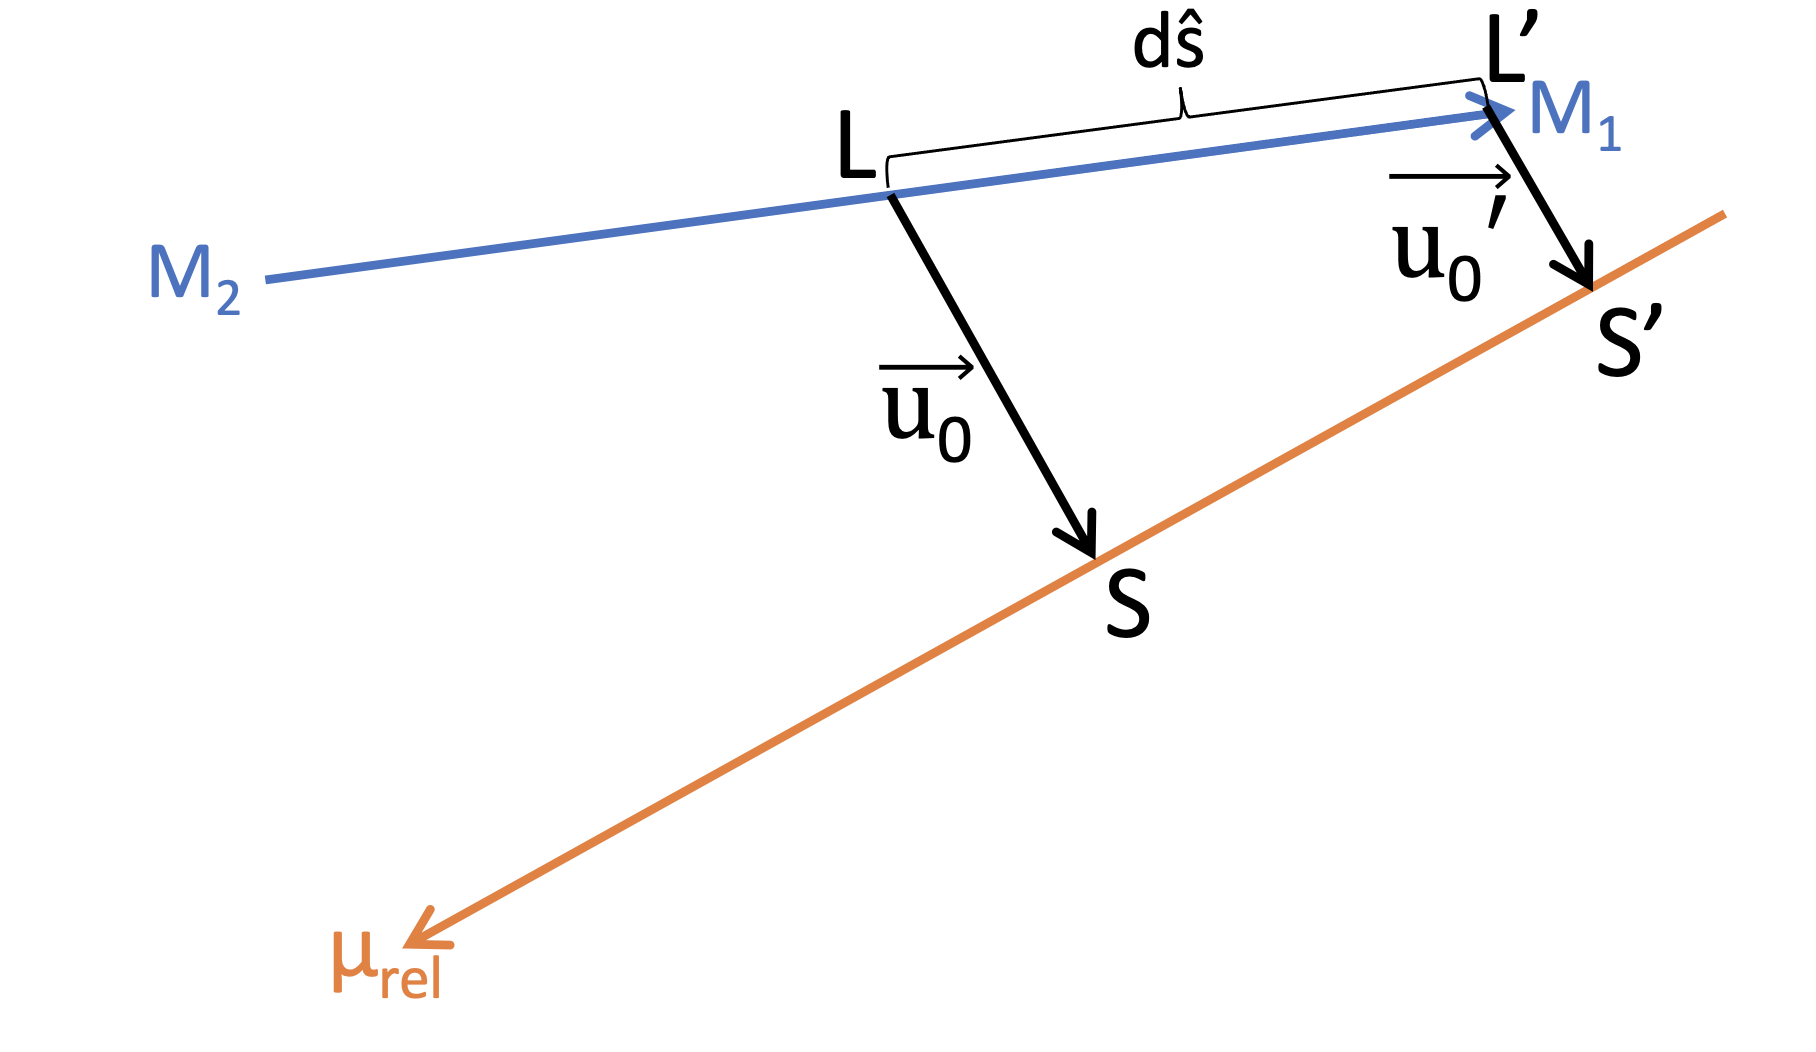
\includegraphics[scale=0.3]{figures/psbl_coord_transform.png}
    \caption{PSBL geometry where blue is the binary axis and orange is the source moving by with relative proper motion $\mu_{rel}$. We're transforming from $L$ to $L'$ where $L'$ is further along in the direction of $\hat{s}$ by $d$. The source's point of closest approach to $L$ is $S$ at a distance $u_0$ at time $t_0$. The source's point of closest approach to $L'$ is $S'$ at a distance $u_0'$ at time $t_0'$.}
    \label{fig:psbl coord transform}
\end{figure}
We're interested in $\vect{u}_0'$ in terms of $\vect{u}_0$.
\begin{eqnarray}
    \vect{u}_0' &=& S'^{R'} - L'^{R'} = (S'^R - d\hat{s}) - (L'^R - d\hat{s}) = S'^R - L'^R \\
    \label{eq: u0' vectors}
    \vect{u}_0' &=& \vect{u}_0 + \frac{\vect{\mu}_{rel}}{\theta_E}(t_0' - t_0) - d\hat{s}
\end{eqnarray}
Let's break this into components where:
\begin{eqnarray}
    \vect{\mu}_{rel} &=& [\mu_{rel}\cos\theta_{\mu}, \mu_{rel}\sin\theta_{\mu}] \\
    \hat{s} &=& [\cos\theta_{s}, \sin\theta_{s}]
\end{eqnarray}
Where $\theta_{\mu}$ is the angle from North to $\vect{\mu}_{rel}$ and $\theta_s$ is the angle from North to the binary axis, East of North. (Note that choosing North as our reference will not affect the final answer. Another reference could be chosen). 
So in components:
\begin{eqnarray}
\label{eq: u0', x}
    u_{0, E}' &=& u_{0, E} + \mu_{rel}\cos\theta_{\mu}\Big(\frac{t_0' - t_0}{\theta_E}\Big) - d\cos\theta_s \\
\label{eq: u0', y}
    u_{0, N}' &=& u_{0, N} + \mu_{rel}\sin\theta_{\mu}\Big(\frac{t_0' - t_0}{\theta_E}\Big) - d\sin\theta_s
\end{eqnarray}

The angle between $\vect{\mu}_{rel}$ and the binary axis ($\vect{s}$) is
\begin{equation}
    \phi = \theta_s - \theta_{\mu}.
\end{equation}
We will also be concerned with the angle to $\vect{u}_0$ from North ($\theta_u$). By definition it is always 90$^{\circ}$ off from $\theta_{\mu}$, but it is sometimes +90$^{\circ}$ and sometimes -90$^{\circ}$. We can find this sign by taking the cross product of $\hat{\mu}_{rel} \times \hat{u}_0$ and dotting the result with $\hat{z}$. $\hat{z}$ is a positive unit vector into the page.
\begin{equation}
\label{eq: C}
    C \equiv (\hat{\mu}_{rel} \times \hat{u}_0) \cdot \hat{z}
\end{equation}
where $C$ is -1 or 1. Since $\hat{z}$ is positive into the page, we subtract the result of the cross product
\begin{equation}
\label{eq: theta_u to theta_mu}
    \theta_u = \theta_{\mu} - 90^{\circ}C
\end{equation}
We can now take Eq.~\ref{eq: u0' vectors} and define the components as their magnitudes times cos/sin of angles:
\begin{eqnarray}
\label{eq: u0'cos}
    u_{0}'\cos\theta_{u'} &=& u_{0}\cos\theta_u + \mu_{rel}\cos\theta_{\mu}\Big(\frac{t_0' - t_0}{\theta_E}\Big) - d\cos\theta_s \\
\label{eq: u0'sin}
    u_{0}'\sin\theta_{u'} &=& u_{0}\sin\theta_u + \mu_{rel}\sin\theta_{\mu}\Big(\frac{t_0' - t_0}{\theta_E}\Big) - d\sin\theta_s
\end{eqnarray}
Where $\theta_{u'}$ is the angle from North to $u_0'$. $u_0$ will always be parallel to $u_0'$, but they may be opposite directions. So
\begin{equation}
    \theta_{u'} = \theta_u + 180^{\circ}F
\end{equation}
where F = 0 if $u_0'$ and $u_0$ are parallel and F = 1 if they are antiparallel. Hence
\begin{eqnarray}
    \sin\theta_{u'} &=& G\sin\theta_u \\
    \cos\theta_{u'} &=& G\cos\theta_u
\end{eqnarray}
where G = -1 if F = 1 and G = 1 if F = 0.
Plugging into Eqs \ref{eq: u0'cos} and \ref{eq: u0'sin}:
%\begin{eqnarray}
%    u_{0}'G\cos(\theta_{u}) &=& u_{0}\cos(\theta_u) + \mu_{rel}\cos(\theta_{\mu})\Big(\frac{t_0' - t_0}{\theta_E}\Big) - d\cos(\theta_s) \\
%    u_{0}'G\sin(\theta_{u}) &=& u_{0}\sin(\theta_u) + \mu_{rel}\sin(\theta_{\mu})\Big(\frac{t_0' - t_0}{\theta_E}\Big) - d\sin(\theta_s)
%\end{eqnarray}
\begin{eqnarray}
    u_{0}'G - u_0 &=& \frac{1}{\cos\theta_{u}}\Big(\mu_{rel}\cos\theta_{\mu}\Big(\frac{t_0' - t_0}{\theta_E}\Big) - d\cos\theta_s\Big) \\
    u_{0}'G - u_0&=&\frac{1}{\sin\theta_{u}}\Big(\mu_{rel}\sin\theta_{\mu}\Big(\frac{t_0' - t_0}{\theta_E}\Big) - d\sin\theta_s\Big)
\end{eqnarray}
We can also simplify 
\begin{eqnarray}
    \cos\theta_u &=& \cos(\theta_\mu - 90^{\circ}C) = C\sin\theta_{\mu} \\
    \sin\theta_u &=& \sin(\theta_\mu - 90^{\circ}C) = -C\cos\theta_{\mu}
\end{eqnarray}
since $C$ is either -1 or 1. Plugging that in:
\begin{eqnarray}
\label{eq: u0' - u0 from x}
    u_{0}'G - u_0 &=& \frac{1}{C}\Big(\mu_{rel}\frac{1}{\tan\theta_{\mu}}\Big(\frac{t_0' - t_0}{\theta_E}\Big) - d\frac{\cos\theta_s}{\sin\theta_{\mu}}\Big) \\
    \label{eq: u0' - u0 from y}
    u_{0}'G - u_0&=&-\frac{1}{C}\Big(\mu_{rel}\tan\theta_{\mu}\Big(\frac{t_0' - t_0}{\theta_E}\Big) - d\frac{\sin\theta_s}{\cos\theta_{\mu}}\Big)
\end{eqnarray}
We can set these equal to simplify. Some useful identities we'll use are:
\begin{eqnarray}
\label{eq: sin(theta_s) convention}
    \sin\theta_s &=& \sin(\theta_{\mu} + \phi) = \cos\phi\sin\theta_{\mu} + \cos\theta_{\mu}\sin\phi \\
\label{eq: cos(theta_s) convention}
    \cos\theta_s &=& \cos(\theta_{\mu} + \phi) = \cos\phi\cos\theta_{\mu} - \sin\phi\sin\theta_{\mu} \\
    \rightarrow \frac{\sin\theta_s}{\cos\theta_{\mu}} &=& \cos\phi\tan\theta_{\mu} + \sin\phi \\
    \frac{\cos\theta_s}{\sin\theta_{\mu}} &=& \frac{\cos\phi}{\tan\theta_{\mu}} - \sin\phi \\
    \rightarrow \frac{\sin\theta_s}{\cos\theta_{\mu}} + \frac{\cos\theta_s}{\sin\theta_{\mu}} &=& \cos\phi\Big(\frac{1}{\tan\theta_{\mu}} + \tan\theta_{\mu}\Big),
\end{eqnarray}
Setting Eq \ref{eq: u0' - u0 from x} equal to Eq \ref{eq: u0' - u0 from y} and simplifying:
\begin{eqnarray}
    \mu_{rel}\Big(\frac{t_0' - t_0}{\theta_E}\Big)\Big(\frac{1}{\tan\theta_{\mu}} + \tan\theta_{\mu}\Big) &=& d\Big( \frac{\sin\theta_s}{\cos\theta_{\mu}} + \frac{\cos\theta_s}{\sin\theta_{\mu}}\Big) \\
    \label{eq: mu_rel, ts, phi relation}
    \mu_{rel}\Big(\frac{t_0' - t_0}{\theta_E}\Big) &=& d \cos\phi
\end{eqnarray}
We can now use this relation in Eqs \ref{eq: u0', x} and \ref{eq: u0', y}. Starting with the E-component:
\begin{eqnarray}
\label{eq: u0x'}
    u_{0, E}' &=& u_{0, E} + d\cos\theta_{\mu}\cos\phi - d\cos\theta_s \\
    u_{0, E}' &=& u_{0, E} + d(\cos\theta_{\mu}\cos\phi - (\cos\phi\cos\theta_{\mu} - \sin\theta_{\mu}\sin\phi))\\
\label{eq: u0x' simplified}
    u_{0, E}' &=& u_{0, E} + d\sin\theta_{\mu}\sin\phi
\end{eqnarray}
Similarly for the N-component:
\begin{eqnarray}
\label{eq: u0y'}
    u_{0, N}' &=& u_{0, N} + d\sin\theta_{\mu}\cos\phi - d\sin\theta_s \\
    u_{0, N}' &=& u_{0, N} + d(\sin\theta_{\mu}\cos\phi - (\cos\phi\sin\theta_{\mu} + \cos\theta_{\mu}\sin\phi)) \\
    \label{eq: u0y' simplified}
    u_{0, N}' &=& u_{0, N}  - d\cos\theta_{\mu}\sin\phi.
\end{eqnarray}
We can use Eq. \ref{eq: theta_u to theta_mu}:
\begin{eqnarray}
\label{sin theta_mu conversion}
    \sin\theta_{\mu} &=& \sin(\theta_u + 90^{\circ}C) = C\cos\theta_u = C\hat{u}_{0,E} \\
\label{cos theta_mu conversion}
    \cos\theta_{\mu} &=& \cos(\theta_u + 90^{\circ}C) = -C\sin\theta_u = -C\hat{u}_{0,N}
\end{eqnarray}
Hence:
\begin{eqnarray}
    u_{0, E}' &=& u_{0, E} +Cd\sin\phi\hat{u}_{0,E} \\
    u_{0, N}' &=& u_{0, N} +Cd\sin\phi\hat{u}_{0,N}
\end{eqnarray}
Putting those together:
\begin{equation}
\label{eq: u0 transform general}
    \boxed{\vect{u_0}' = \vect{u_0} + Cd\sin\phi\hat{u}_0}.
\end{equation}

We may also want to go the opposite direction. To do so we can define an equivalent of Eq. \ref{eq: C} for $\vec{u}_0'$:
\begin{equation}
    C' \equiv (\hat{\mu}_{rel} \times \hat{u}_0') \cdot \hat{z}
\end{equation}
So Eqs. \ref{sin theta_mu conversion} and \ref{cos theta_mu conversion} become
\begin{eqnarray}
    \sin\theta_{\mu} &=& \sin(\theta_{u'} + 90^{\circ}C') = C'\cos\theta_{u'} = C'\hat{u}'_{0,E} \\
    \cos\theta_{\mu} &=& \cos(\theta_{u'} + 90^{\circ}C') = -C'\sin\theta_{u'} = -C'\hat{u}'_{0,N}
\end{eqnarray}
Hence
\begin{eqnarray}
    u_{0, E}' &=& u_{0, E} +C'd\sin\phi\hat{u}'_{0,E} \\
    u_{0, N}' &=& u_{0, N} +C'd\sin\phi\hat{u}'_{0,N} \\
    \vect{u}_0' &=& \vect{u}_0 + C'd\sin\phi\hat{u}'_0
\end{eqnarray}
So Eq. \ref{eq: u0 transform general} becomes
\begin{equation}
    \label{eq: u0' transform general}
    \boxed{\vect{u}_0 = \vect{u}_0' - C'd\sin\phi\hat{u}'_0}.
\end{equation}

\subsection{Standard Coordinate Transforms}
\label{sec: standard transforms}
\subsubsection{Between Geometric Midpoint and Primary}
The separation in mas between the two lenses is $\vect{a}$ pointing towards the primary. In units of $\theta_{E}$, it's $\vect{s} \equiv \frac{\vect{a}}{\theta_E}$. So the vector from the geometric midpoint to the primary is $\frac{\vect{s}}{2}$. Hence Eq. \ref{eq: u0 transform general} becomes
\begin{equation}
    \vect{u_{\textrm{prim},0}} = \vect{u_{\textrm{geo}, 0}} + C\frac{a}{2\theta_E}\sin\phi\hat{u}_{\textrm{geo}, 0}.
\end{equation}
When transforming from primary to geometric midpoint, Eq. \ref{eq: u0' transform general} becomes:
\begin{equation}
    \vect{u_{\textrm{geo},0}} = \vect{u_{\textrm{prim},0}} - C'\frac{a}{2\theta_E}\sin\phi\hat{u}_{\textrm{prim}, 0}.
\end{equation}

\subsubsection{Between Geometric Midpoint and Center of Mass}
Following the derivation in \cite{Casey_Thesis}, Section 6.4.1, the separation between the geometric midpoint and center of mass in units of Einstein radii becomes:
\begin{equation}
    \vect{d} = \vect{s}\frac{1 - q}{2(1 + q)} \equiv \vect{s}q'.
\end{equation}
Hence Eq. \ref{eq: u0 transform general} becomes
\begin{equation}
    \vect{u_{\textrm{com}}, 0} = \vect{u_{ \textrm{geo}, 0}} + Csq'\sin\phi\hat{u}_{\textrm{geo}, 0}.
\end{equation}
When transforming from primary to geometric midpoint, Eq. \ref{eq: u0' transform general} becomes:
\begin{equation}
    \vect{u_{\textrm{geo},0}} = \vect{u_{\textrm{com},0}} - C'sq'\sin\phi\hat{u}_{\textrm{com}, 0}.
\end{equation}
If the secondary is more massive, then the center of mass is closer to the secondary than the primary, so the two equations will swtich.



\section{$\lowercase{t}_0$ transformation}
\label{sec:t0}

Along with a change in the distance of closest approach, there is a change of when the closest approach occurs. In Fig. \ref{fig:psbl geometry projection}, the source is at $S$ at time $t_0$ and at $S'$ at time $t_0'$. Since the source is moving with relative proper motion $\boldsymbol{\mu_{rel}}$, we know:
\begin{equation}
    \label{eq: motion eq}
    S' - S = \frac{\vect{\mu_{rel}}}{\theta_E}(t_0' - t_0)
\end{equation}
The source moves across the Einstein radius ($\theta_E$) in time $t_E$, so:
\begin{equation}
    \mu_{rel} = \frac{\theta_E}{t_E}
\end{equation}
We can find $S' - S$ by projecting the binary axis onto $\vec{\mu}_{rel}$. The two are separated by angle $\phi$, so 
\begin{equation}
    S' - S = dcos\phi \hat{\mu}_{rel}
\end{equation}
Plugging this into Eq. \ref{eq: motion eq}, we find
\begin{eqnarray}
    dcos\phi \hat{\mu}_{rel} &=& \frac{\vect{\mu_{rel}}}{\theta_E}(t_0' - t_0) \\
    dcos\phi \hat{\mu}_{rel} &=& \frac{1}{t_E}(t_0' - t_0) \hat{\mu}_{rel}
\end{eqnarray}
\begin{equation}
\label{eq: t0 transform}
    \boxed{t_0' = t_0 + t_E d cos\phi}
\end{equation}

\begin{figure}
    \centering
    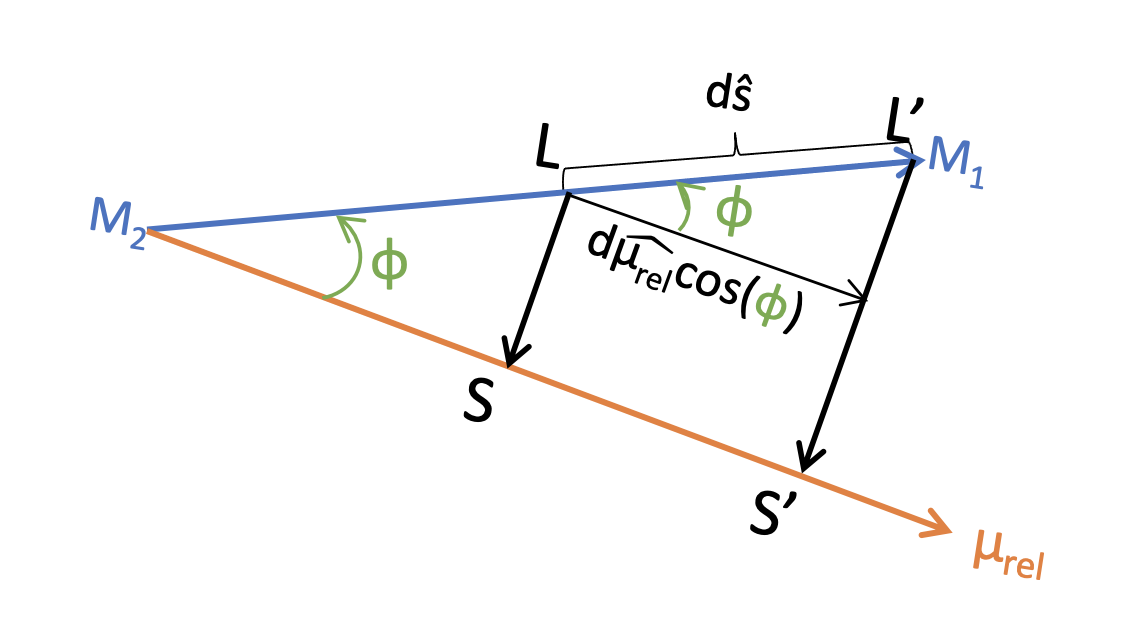
\includegraphics[scale=0.6]{figures/psbl_geometry_projection.png}
    \caption{Similar to Fig. \ref{fig:psbl coord transform} but with the angle, $\phi$ between $\vect{\mu_{rel}}$ and the binary axis ($\vect{s}$) marked. $\phi < 90^{\circ}$ chosen for ease of visualization. The projection of $d\hat{s}$ onto $\vect{\mu_{rel}}$ is dcos$\phi\hat{\mu}_{rel}$.}
    \label{fig:psbl geometry projection}
\end{figure}

\subsection{Standard Coordinate Transforms}
As described in Section \ref{sec: standard transforms}, for a geometric midpoint $\leftrightarrow$ primary center transformation Eq. \ref{eq: t0 transform} becomes
\begin{eqnarray}
    t_{prim, 0} = t_{geo, 0} + t_E\frac{a}{2\theta_E}cos\phi
\end{eqnarray}
and for a geometric midpoint $\leftrightarrow$ center of mass transformation Eq. \ref{eq: t0 transform} becomes
\begin{eqnarray}
    t_{prim, 0}  = t_{geo, 0} + t_Esq'cos\phi
\end{eqnarray}


\bibliographystyle{aasjournalv7}
\bibliography{main.bib}

\end{document}
